% \iffalse meta-comment
%
% Copyright (C) \the\year by Liu Benyuan <liubenyuan@gmail.com>
% This file may be distributed and/or modified under the
% conditions of the LaTeX Project Public License, either
% version 1.2 of this license or (at your option) any later
% version. The latest version of this license is in:
%
% http://www.latex-project.org/lppl.txt
%
% and version 1.2 or later is part of all distributions of
% LaTeX version 1999/12/01 or later.
%
% \fi
% 
% \iffalse
% <package>\NeedsTeXFormat{LaTeX2e}[1999/12/01]
% <package>\ProvidesPackage{nudtpaper}
% <package>[2015/05/12 v2.5 By Liu Benyuan <liubenyuan@gmail.com>]
%<*driver>
\ProvidesFile{nudtpaper.dtx}[2015/05/12 v2.5 NUDT]
\documentclass[11pt]{ltxdoc}
\usepackage{nudtx}
\EnableCrossrefs
\CodelineIndex
\RecordChanges
\begin{document}
  \DocInput{\jobname.dtx}
\end{document}
%</driver>
% \fi
% 
% \def\thuthesis{\textsc{Thu}\-\textsc{Thesis}}
% \def\nudtpaper{\textsc{Nudt}\-\textsc{Paper}}
% 
% \CheckSum{1217}
% \CharacterTable
%  {Upper-case    \A\B\C\D\E\F\G\H\I\J\K\L\M\N\O\P\Q\R\S\T\U\V\W\X\Y\Z
%   Lower-case    \a\b\c\d\e\f\g\h\i\j\k\l\m\n\o\p\q\r\s\t\u\v\w\x\y\z
%   Digits        \0\1\2\3\4\5\6\7\8\9
%   Exclamation   \!     Double quote  \"     Hash (number) \#
%   Dollar        \$     Percent       \%     Ampersand     \&
%   Acute accent  \'     Left paren    \(     Right paren   \)
%   Asterisk      \*     Plus          \+     Comma         \,
%   Minus         \-     Point         \.     Solidus       \/
%   Colon         \:     Semicolon     \;     Less than     \<
%   Equals        \=     Greater than  \>     Question mark \?
%   Commercial at \@     Left bracket  \[     Backslash     \\
%   Right bracket \]     Circumflex    \^     Underscore    \_
%   Grave accent  \`     Left brace    \{     Vertical bar  \|
%   Right brace   \}     Tilde         \~}
%
% \changes{v0.99}{2009/08/12}{Initial Release}
%
% \GetFileInfo{\jobname.dtx}
% 
% \DoNotIndex{\begin,\end,\begingroup,\endgroup}
% \DoNotIndex{\ifx,\ifdim,\ifnum,\ifcase,\else,\or,\fi}
% \DoNotIndex{\let,\def,\xdef,\newcommand,\renewcommand}
% \DoNotIndex{\expandafter,\csname,\endcsname,\relax,\protect}
% \DoNotIndex{\Huge,\huge,\LARGE,\Large,\large,\normalsize}
% \DoNotIndex{\small,\footnotesize,\scriptsize,\tiny}
% \DoNotIndex{\normalfont,\bfseries,\slshape,\interlinepenalty}
% \DoNotIndex{\hfil,\par,\hskip,\vskip,\vspace,\quad}
% \DoNotIndex{\centering,\raggedright}
% \DoNotIndex{\c@secnumdepth,\@startsection,\@setfontsize}
% \DoNotIndex{\ ,\@plus,\@minus,\p@,\z@,\@m,\@M,\@ne,\m@ne}
% \DoNotIndex{\@@par,\DeclareOperation,\RequirePackage,\LoadClass}
% \DoNotIndex{\AtBeginDocument,\AtEndDocument}
%
% \IndexPrologue{\section*{索引}%
%    \addcontentsline{toc}{section}{索~~~~引}}
% \GlossaryPrologue{\section*{修改记录}%
%    \addcontentsline{toc}{section}{修改记录}}
%
% \renewcommand{\abstractname}{摘~~要}
% \renewcommand{\contentsname}{目~~录}
%
% \title{\textsc{NUDTpaper:}\,\,NUDT研究生学位论文\LaTeX{}模板使用手册\thanks{NUDT \LaTeX{} Thesis Template}}
% \author{刘本源 \\ \texttt{Liubenyuan@gmail.com}}
% \date{\fileversion\ (\filedate)}
%
% \maketitle
% \thispagestyle{empty}
%
% \begin{abstract}
% 本模板旨在提供规范的国防科学技术大学\LaTeX{}写作模板环境,
% 现支持硕士/博士学位论文格式,可以自动生成盲评、制作A3封面。
% \end{abstract}
%
% \vspace{2cm}
% \def\abstractname{免责声明}
% \begin{abstract}\noindent
% \begin{enumerate}
% \item 本模板的发布遵守 \LaTeX{} Project Public License,使用前请认真阅读协议内容
% \item 本模板创立参照官方严格的论文写作手册,并同时参照硕士/博士学位论文\textbf{doc}文档对比修改
% \item 国防科学技术大学对论文写作提供写作指南与官方\textbf{doc}模板,
% 同时提供官方的\LaTeX{}模板,本模板的出发点是方便大家使用专业的高效的论文书写工具,
% 其有点在于注重排版质量、命令规范、使用方便、更新及时,符合论文撰写说明。
% 但任何由于使用本模板而引起的论文格式审查问题均与本模板作者无关。
% \item 任何个人或组织均可以本模板为基础进行修改、扩展,生成新的专用模板,但请严格遵
% 守\LaTeX{} Project Public License 协议
% \item 欢迎提出修改意见
% \end{enumerate}
% \end{abstract}
%
% \clearpage
% \tableofcontents
%
% \clearpage
% \pagenumbering{arabic}
% \pagestyle{mainpage}
%
% \section{快速上手}
% \begin{description}
% \item[安装\TeX] 下载最新的\TeX{}live或者C\TeX{}并安装
% \item[字体] 用户需要具备\verb|simsun.ttf|, \verb|simhei.ttf|, \verb|simkai.ttf|,
% \verb|STZHONGS.TTF|, 上述字体都是windows自带的; 除此之外,在网上搜索(或者C\TeX{}
% 论坛)``Adobe Opentype 中文字体'',一搜一大把,确保下载下来Adobe的四款OTF字体:
% 宋,黑,仿宋,楷体。Linux用户可将上述字体复制到\verb|/usr/share/fonts/TTF|下。
% 最新更新:用户可以考虑使用方正字体生成更为漂亮(颜色深均匀)的论文排版。
% 这三个选项分别为\verb|ttf|、\verb|otf|和\verb|fz|。
% \item[试一试] 解压缩下载的模板,双击makepdf.bat(祈祷一下),如果生成了
% \verb|thesis.pdf|$\rightarrow$
% \item[那么我的那些常用的包都在么?] 你会想我的{\bf Trans}论文可以无缝
% 的复制过来么? 对于这一点,你可以修改\verb|mynudt.sty|来实现。但是{\hei 注意},大部分包
% 都在模板中了,而且{\hei 切记切记},不要擅自改动字体等版面设计,我们继续看$\rightarrow$
% \item[咦,数学公式不是很美观呀] 笔者{\hei 强烈}建议用户使用{\bf mtpro2}宏包的,怎么使用,
% 又有哪些好处,参见bookzh.sty吧!不会错的。好了,我们专注于内容本身吧$\rightarrow$
% \item[开始写了] 所有文件均采用UTF8编码,因此要保证你的\TeX{}编辑器
% (winedt, texworks, texmaker, vim, 记事本($\cdots{}$)等)支持这种编码,
% (经过一番搜索设置后)打开\verb|thesis.tex|,如果看到的是中文$\rightarrow$
% \item[漫长的写作] 手边准备着\LaTeX{}的常用帮助文档(数学,图表,引用等),
% 结合你喜欢的文献管理软件(JabRef等), 漫长的\texttt{编辑,编译,修改,编辑,
% 编译$\cdots$}过程之后,突然有一天发现你写完了$\rightarrow$
% \item[校订] 经过老师师兄师弟师妹齐心协力校正之后,你所做的只是:
% \texttt{生成明评论文,制作明评封面,生成盲评论文,制作盲评封面},
% 装订,上交$\rightarrow$
% \end{description}
% {\color{magenta} Done!}
%
% \section{模板介绍}
%
% \textsc{NUDTpaper} 旨在帮助并且推广\LaTeX{}在国防科技大学论文中的应用,
% 本文将尽可能帮助用户掌握\textsc{NUDTpaper}的安装方法,
% 如果仍旧有不清晰的地方可以参考样例文件或者
% 给作者邮件\footnote{liubenyuan@gmail.com},感兴趣的同学可以帮忙维护模板,
% 这个模板首先符合官方的设计要求,希望同学们在使用后能够提出你们的修改意见。
% 该模板很大程度上参考了6院黄老师sofoot的国防科大博士论文模板,
% 哈工大的\LaTeX{}模板以及清华的Thuthesis
% \footnote{主页:\url{http://thuthesis.sourceforge.net}},
% 有很多使用的帮助、\verb|.cls|中的命令以及版面设置均来自Thuthesis和sofoot的模板,
% 对此的引用表示感谢。
%
% {\color{blue}\fs 模板的作用在于减轻论文写作过程中格式调整的时间,
% 其前提就是遵守模板的用法,不提倡手动更改格式,不建议正文中使用
% 手动调节版面的命令,尤其禁止修改行距和使用\verb|\normalsize|,
% 否则即使使用了\textsc{NUDTpaper}也难以保证输出的论文符合学校规范。}
%
% \section{安装}
% \label{sec:install}
%
% \subsection{下载}
% \textsc{NUDTpaper} 主页:\url{http://nudtpaper.googlecode.com}。
% 模板的更新信息发布在\href{http://bbs.ctex.org}{Ctex论坛}。
% \nudtpaper{}的开发版本同样可以在\textsc{gitorious}上获得。
%
% \subsection{模板的组成部分}
% 下表列出了 \nudtpaper{} 的主要文件及其功能介绍,学习模板的最好办法
% 就是参考thesis.pdf!
% \begin{center}
% \begin{longtable}{l|p{8cm}}
% \toprule
% {\hei 文件(夹)} & {\hei 功能描述}\\\midrule
% \endfirsthead
% \toprule
% {\hei 文件(夹)} & {\hei 功能描述}\\\midrule
% \endhead
% \endfoot
% \endlastfoot
% nudtpaper.ins & 模板驱动文件 \\
% nudtpaper.dtx & 模板文档代码的混合文件\\
% nudtpaper.cls & 模板类文件\\
% nudtpaper.cfg & 模板配置文件\\
% thesis.bib & 参考文献样式文件\\
% \hline
% mynudt.sty & 在这里添加你自己的宏包 \\
% thesis.tex & 示例文档主文件\\
% ref/ & 示例文档参考文献目录\\
% data/ & 示例文档章节具体内容\\
% figures/ & 示例文档图片路径\\
% \textbf{nudtpaper.pdf} & 用户手册(本文档)\\
% \textbf{thesis.pdf} & 示例文档 \\
% \bottomrule
% \end{longtable}
% \end{center}
%
% \subsection{\TeX{}系统的选择}
% 有网络环境的用户推荐安装\href{http://www.tug.org/texlive}{\TeX{}live},
% \href{http://miktex.org}{MiKTeX}或者\href{http://www.ctex.org}{C\TeX},
% 对于无网络环境的,主要是针对教研室用户,推荐{\TeX{}live}或者C\TeX{}完整版,安装
% 过程很简单,一路下一步即可,但是需要\textbf{注意:}
%
% \begin{description}
% \item[字体] TTF选项默认调用Windows系统字体,其中楷体、仿宋需要安装Office;OTF选项需要
% Adobe的商业字体(可以使你的论文更加漂亮!),这些中文字体(宋,黑,仿宋,楷体)可以从
% \href{http://dl.getdropbox.com/u/857066/adobe_chinese_otf.7z}{这里下载},
% 如果上述链接不能使用,请搜索\textsc{Adobe Opentype 中文字体}自行下载。
% 英文字体使用Windows自带。起始更推荐几款Times(Arial)类似的OTF英文字体,可以使用
% 更多排版、段落的字体特性。
% \item[粗宋] 模板中在需要宋体加黑的地方需要使用\textbf{华文中宋}, 即STZHONGS.TTF。
% \item[xeCJK] 无网络环境中,C\TeX{}完整版和\TeX{}live最新版都包括了需要的xeCJK版本。
% \end{description}
%
% \subsection{使用模板}
% \label{sec:install-cls}
% {\hei 注:默认的发行版本已经包含了可以使用的模板环境,
% 包括编译好的cls以及论文样例源文件,
% 想快速上手的话,可以直接参看\verb|thesis.tex|,进行修改。
% 写作的过程就是将你的论文的内容放到\verb|data|文件夹中,
% 图片放到\verb|figures|文件夹中,用\textsc{jabref}修改\verb|thesis.bib|即可。}
%
% 当用户需要编译生成自己的PDF版论文时,需要依次输入:(注意了,如果不是使用nomencl,
% 则无需使用第二个命令)
% \begin{shell}
% $ xelatex thesis
% $ # makeindex -s nomencl.ist -o thesis.nls thesis.nlo
% $ bibtex thesis
% $ bibtex thesis
% $ xelatex thesis
% $ xelatex thesis
% \end{shell}
%
% 而为了简化用户使用,模板中提供了快捷脚本文件:
% \begin{shell}
% # 下面命令可以直接生成thesis.pdf,你可能只需要这步
% C:\> makepdf.bat
% # linux用户可以直接使用makefile
% $ make pdf
% \end{shell}
% 现在,就要进入激动人心的写作过程了。
%
% \section{使用说明}
% \label{sec:how-to-use}
% 首先,一篇论文(电子信息工程专业为例),主要的构成就是
% 封面导言,正文,表格,图片,公式,
% 交叉引用及文献索引这五部分,下面将分别详细讲解。
%
% \label{sec:howtoask}
% 在开始之前,先问自己几个问题:
% \begin{compactenum}
% \item 我是不是已经掌握了 \LaTeX{} 基础知识?
% \item 我是不是认真地阅读了模板文档?
% \item 周围有没有同学可以帮我?
% \end{compactenum}
% 更推荐用户去阅读示例文档的源代码,改写会给你一个快速的开始。
%
% \subsection{示例文件}
% \label{sec:example}
% 该示例文件是顶层的文件,包括论文属性设置、章节的安排、参考文献附录等。
% 细节用户可以参考\verb|thesis.tex|和\verb|data/|文件夹。
%
% \subsubsection{模板选项}
%
% 论文的第一句话是调用模板:
% \changes{v2.0}{2010/11/10}{增加盲评的说明}
%
%    \begin{macrocode}
%<thesis>%1. 规范硕士导言
%<thesis>% \documentclass[master,ttf]{nudtpaper}
%<thesis>%2. 规范博士导言
%<thesis>% \documentclass[doctor,twoside,ttf]{nudtpaper}
%<thesis>%3. 建议使用OTF字体获得较好的页面显示效果
%<thesis>%   OTF字体从网上获得,各个系统名称统一。
%<thesis>%   如果你下载的是最新的(1201)OTF英文字体,建议修改nudtpaper.cls,使用
%<thesis>%   Times New Roman PS Std
%<thesis>% \documentclass[doctor,twoside,otf]{nudtpaper}
%<thesis>%   另外,新版的论文模板提供了方正字体选项FZ,效果也不错哦
%<thesis>% \documentclass[doctor,twoside,fz]{nudtpaper}
%<thesis>%4. 如果想生成盲评,传递anon即可,仍需修改个人成果部分
%<thesis>% \documentclass[master,otf,anon]{nudtpaper}
%<thesis>%
%    \end{macrocode}
%    \begin{macrocode}
%<*thesis>
\documentclass[master,otf]{nudtpaper}
\usepackage{mynudt}

%</thesis>
%    \end{macrocode}
%
% 模板的参数设置(开关)描述见:
%
%\begin{description}
%\item[master,doctor]
% 硕士论文用master,博士论文就用doctor
%\item[twoside]
% 指定论文为单面打印还是双面打印,当使用\verb|twoside|选项之后,
% 论文会将章节开在奇数页右手边,默认为\verb|openany|单面打印。
%\item[ttf,otf]
% 决定使用何种字体,TTF默认使用Windows自带的字体,而OTF则使用Adobe的字体(需要下载),
% TTF字体的优势是满足学校论文对于字体的要求,缺点是制作出来的PDF文件在浏览时可能发虚,
% 而OTF字体屏幕显示饱满,而且字体有很多选项可以方便\XeTeX{}排版。推荐使用\textbf{otf}
% 选项。不论何种选项,都需要安装宋体中宋(STZHONGSONG)字体(Windows自带)。
%\item[anon]
% 是否为盲评版本,如需盲评,请加上anon。
%\end{description}
%
% 如果需要使用自己定义的命令、宏包,请放于\verb|mynudt.sty|中。
% 事实上,该文件中已经添加了很多有用的宏包和命令,你可以参照修改。
% 这些之所以没有放到模板中,一则为了简洁,二则赋予用户在格式之外更多的自由。
% 里面的宏包有:代码高亮、算法环境、向量命令等,请仔细查看。
%
% 样例文件默认的是硕士论文(master),OTF字体(otf)。
%
% \subsubsection{封面导言}
% 官方模板中设计论文题目、作者等信息可以跟填空一样完成:
%
% \begin{description}
% \item[论文封头]
% 主要有四部分内容,中图分类号,学号,论文密级和UDC。
% 密级分为:\textbf{秘密} 或者 \textbf{公开}。
%    \begin{macrocode}
%<*thesis>
\classification{TP957}
\serialno{0123456}
\confidentiality{公开}
\UDC{}
%</thesis>
%    \end{macrocode}
%
% \item[论文题目,作者,日期]
% 分别包括中文和英文两部分,由于论文题目可能超过1行,
% 我们提供额外的一个命令\verb|\displaytitle|用来在
% 授权书中填入(限定为)单行的题目; 中文日期需要中文输入大写,英文日期为月年,
% 在论文最终完成后,请\textbf{手动}设定日期。
% \changes{v2.5}{2015/05/11}{修改英文作者和导师的格式,姓大写}
% \changes{v2.5}{2015/05/11}{英文导师前缀为Prof.}
%
%    \begin{macrocode}
%<*thesis>
\title{国防科大学位论文\LaTeX{}模板\\
使用手册}
\displaytitle{国防科学技术大学学位论文\LaTeX{}模板}
\author{张三}
\zhdate{\zhtoday}
\entitle{How to Use the \LaTeX{} Document Class for NUDT Dissertations}
\enauthor{ZHANG San}
\endate{\entoday}
%</thesis>
%    \end{macrocode}
%
% \item[论文分类及其他]
% 主要是作者的学科类别,研究方向,导师信息等。
% 每一项都包括中英文信息:
%
%    \begin{macrocode}
%<*thesis>
\subject{通信与信息工程}
\ensubject{Information and Communication Engineering}
\researchfield{自动目标识别与模糊工程}
\supervisor{李四\quad{}教授}
\cosupervisor{王五\quad{}副教授} % 没有就空着
\ensupervisor{Prof. LI Si}
\encosupervisor{}
\papertype{工学}
\enpapertype{Engineering}
%</thesis>
%    \end{macrocode}
%
% \item[中英文摘要]
% 论文中需要写中文以及英文摘要,页码为小写罗马字母,关键字为黑体,
% 英文关键字为\verb|Arial|,
% 模板中定义了相关环境\verb|\cabstract|以及\verb|\eabstract|来书写摘要,
% 以及\verb|\ckeywords|以及\verb|\ekeywords|来写关键字。
% 建议用户将摘要单独放在在\verb|abstract.tex|文件中,
% 在正文中\verb|\begin{cabstract}
近年来,随着互联网技术的发展,在线社交网络已经融入到了人们生活的各方面之中。在线社交网络是现实世界中个体集合和个体之间的连接关系所构成的网络在虚拟网络上的映射,即在线社交网络是真实世界在虚拟网络上的体现与扩展。真实世界中的事件会以信息的形式在社交网络中存在,并且随着用户之间的社交互动传播与演化,并且反作用于现实世界,影响人们的日常行为。在线社交网络拉近了人与人之间的距离,加快了信息传播的速率,丰富了群体的结构关系。因此,在线社交网络成为了社会学、传播学、计算机科学以及系统科学等领域的研究热点。

在线社交网络信息传播分析与自然语言处理、数据挖掘、机器学习、传播学、社会学等学科有着紧密的联系。社交网络中的数据种类繁多、关系结构复杂、信息传播迅速,这些特点使得社交网络中的信息传播分析与传统的信息传播分析有所不同,带来了新的机遇与挑战。本文在已有的研究基础之上,针对社交网络中影响力最大化、实时个性化搜索、文本分类、传播模型学习等问题进行了研究,主要的研究成果如下:
\begin{enumerate}
	\item 在影响力最大化问题方面,本文提出了传播效率最大化问题,并且分析了该问题的复杂性,最后提出了一种反向效率采样算法来解决该问题。传统的影响力最大化问题仅仅考虑了最大化最终的传播范围,而没有考虑节点被激活的时刻,即传播时延。而在实际应用中,如何尽快地使得节点被激活也是十分有意义的。针对上述不足,本研究将传播时延进行了考虑,定义了传播效率函数,提出了传播效率最大化问题。随后,我们证明了该问题是一个NP-难的问题,而且在独立级联模型下计算传播效率的过程是一个\#P-难的问题。我们对传播效率函数进行分析,证明传播效率函数在独立级联模型下是具有子模性的。最后,本研究设计了一种反向传播采样算法来解决该问题。
	\item 在实时个性化搜索方面,本文提出了一种结合语义扩展和质量模型的实时个性化搜索框架。在传统的搜索模式中,往往是用户输入关键词,系统进行检索后返回排序后的结果。而在社交网络中,信息产生速率快,信息以数据流的形式出现,同时,用户希望系统自动地根据用户偏好推送信息。针对这些不足,本研究提出了一种基于语义扩展和文本质量的实时个性化搜索框架,该框架综合考虑了用户的偏好、语义特征和社交属性。我们采用了一种布尔逻辑关键词过滤(Boolean Logic Keyword Filter)的用户模型。该模型依靠外部搜索引擎提供的知识进行建立,建立的用户模型充分利用了查询扩展以及检索结果的重排序来提高推荐结果的相关性。同时我们还使用了一种基于逻辑回归的文本质量模型,该模型利用推文的社交属性来评估其文本的质量,使得返回结果中的文本包含更有用的信息。
	\item 在文本分类方面,本文提出了一种基于文本摘要和卷积神经网络的文本分类方法。社交网络中的文本数据量大,话题种类较多,传统的词袋模型面临着维度爆炸问题。同时社交网络中的文本包含着丰富的上下文关系,传统的分类方法都没有对这个信息进行利用。针对上述不足,我们提出了一种结合词向量模型和卷积神经网络的文本分类算法,该算法控制了文本表示的维度,保留了上下文关系的局部特征。算法包含了文本摘要的提取、同时利用外部语料库训练结果进行词语的向量化以及卷积神经网络。实验证明了算法的正确性和有效性。
	\item 在传播模型学习方面,本文提出了一种基于概率阅读的事件传播模型。在实际应用中,一个事件往往由多条信息组成,因此研究事件的传播分析需要考虑多个传播网络融合的问题。其次,社交网络中的垃圾用户对传播影响范围的计算造成了偏差。因此,需要训练模型对垃圾用户进行过滤,去除这些噪声。最后,信息推送至用户,用户阅读到信息是一个概率性的事件,需要建立模型来计算用户阅读到信息的概率。针对上述问题,我们提出了基于概率阅读的事件传播模型,模型对上述的三个问题进行了综合考虑,进行训练后得到的模型能够真实的反应出事件的传播范围。
\end{enumerate}

综上所述,本文对在线社交网络中的影响力最大化问题、实时个性化搜索、文本分类以及传播模型等关键技术进行了研究,在真实数据集上验证了方法的有效性,对社交网络信息传播提供了理论依据和实际应用方法。
\end{cabstract}
\ckeywords{社交网络; 影响力最大化; 实时个性化搜索; 文本分类; 传播模型}

\begin{eabstract}
Recently, with the development of Internet technology, the online social network plays an important role in people's daily life. The online social network is representation of network which consists of the individuals and the relationships among individuals in the real world, that means online social network is the reflection and extension of real world. The information about the event which happens in the real world will exist in online social network. And it will propagate and evolve with the interactions among the users in online social network. And what's more, it will react on the real world and influence people's behaviors and actions. The online social network narrows the gap between the individuals, accelerates the propagation speed and fertilizes the relationships among individuals. So the online social network becomes one of the research highlights in the field of sociology, communication, computer science, system science, and etc.

The analysis of information diffusion in online social network is related to natural language processing, data mining, machine learning, communication, sociology, and etc. In online social network, there are many types of data, complex relationships and fast propagating information. Those characteristics make it different for information diffusion analysis in online social network from the traditional analysis. It brings new opportunities as well as new challenges. This paper aims at influence maximization, real-time personalized search, text classification and information diffusion learning based on the existing related work. The main achievements are as follows:

\begin{enumerate}
	\item In terms of influence maximization problem, this paper proposes the influence efficiency maximization problem, analyses the complexity of that problem and design a reverse efficiency sampling algorithm to solve that problem. Traditional influence maximization problem only take the final influence into consideration, neglecting the time stamp that node is activated, which is called propagation time delay. While in practical application, it is meaningful to activate nodes as soon as possible. To solve the problem, we take propagation time delay into account, define the influence efficiency function and propose the influence efficiency maximization problem. After that, we prove that problem is NP-hard under independent cascade model. And what's more, the computation of influence efficiency is \#P-hard under independent cascade model. We also prove that the influence efficiency function is submodular. At last, we design a reverse efficiency sampling algorithm to solve the problem.
	\item In the terms of real-time personalized searching, this paper propose a framework for real-time personalized searching which integrates semantic extension and quality model. In traditional information retrieval model, the system returns the re-ranked results based on user input. While in online social network, the information generates in high speed and emerges as data stream. Moreover, it is proper to push information automatically according to user's intention. To solve the problem, we propose a framework for real-time personalized searching that integrates semantic extension and quality model. We adopt a user model based on boolean logic keyword filter. It constructs based on external knowledge base, leverage the query extension to re-rank the results according to the relevance. Furthermore, we utilize a text quality model based on logistic regression. It evaluate text's quality based on the social attributes, making the retrieval text meaningful.
	\item In the terms of text classification, this paper proposes a text classification algorithm based on text summarization and convolutional neural network. In online social network, there are enormous text data and a large variety of topics, so traditional bag-of-word model confronts the problem of dimension explosion. Besides, there is context dependence in the text. While traditional methods make no use of that property. To solve that problem, we propose a text classification algorithm integrating word vector model and convolutional neural network. The algorithm fixes the dimensionality and keep the local feature of the context. The algorithm includes text summary extraction, text vectorization and convolutional neural network. Finally, the experiments verify the effectiveness of the algorithm.
	\item In the terms of diffusion model learning, this paper proposes a diffusion model based on probabilistic reading. In practice, an event consists of many information. So we need to take multiple network convergence into consideration. And furthermore, the spam users in online social network bring noise to the evaluation of influence. So we need to construct a spam user filter to get rid of the noise. Moreover, whether the user receives the information or not when the information is pushed to user's timeline is probabilistic. So we need to model user's reading probability. To solve those problems, we propose a diffusion model based on probabilistic reading, which considers those problems comprehensively. After training, the model can reflect the actual influence of an event.
\end{enumerate}

In a conclusion, this paper aims at influence maximization problem, real-time personalized searching, text classification and diffusion model learning in online social network. We carry out experiments on real world dataset, and the experimental results show the effectiveness of our methods. The methods for information diffusion analysis in online social network are practical.
\end{eabstract}
\ekeywords{Social Network, Influence Maximization, Real-time Personalized Search, Text Classification, Diffusion Model}

|即可。其格式为:
%
% \begin{example}
% \begin{cabstract}
% 中文摘要
% \end{cabstract}
% \ckeywords{关键字}
%
% \begin{eabstract}
% Abstract
% \end{eabstract}
% \ekeywords{Key}
% \end{example}
% \end{description}
%
% \subsubsection{框架构成}
%
% 在定义完论文元素之后,就可以开始写论文正文了。用\LaTeX{}写论文的文件目录构成
% 可以很随意,模板中将图形文件单独放到一个目录中\verb|figure|中,论文正文各个
% 章节置于\verb|data|中;当然也以以\verb|chapter|为目录。
%\changes{v2.2}{2011/05/27}{使用nomencl包管理符号列表}
%\changes{v2.2}{2011/07/08}{默认使用nomencl管理参考文献}
%\changes{v2.2}{2011/09/10}{回复原先使用的denotation方式添加符号列表}
% 
% 如果使用nomencl制作符号列表,在文档开始前要加入\verb|\makenomenclature|命令
% 默认还是使用denotation的方式。nomencl可以参考第二章相关章节,而denote方式
% 请参考\verb|data/denotation.tex|文件(简单的列表环境)。
% 
%<thesis>% 加入makenomenclature命令可用nomencl制作符号列表。
%
%    \begin{macrocode}
%<*thesis> 

\begin{document}
\graphicspath{{figures/}}
%</thesis>
%    \end{macrocode}
% 制作完封面后就是正文四大部分了,分别为:
%
% \begin{compactenum}
% \item frontmatter: 生成目录,图目录,表目录
% \item midmatter: 摘要,符号列表
% \item mainmatter: 正文,致谢,文献,成果
% \item backmatter: 附录
% \end{compactenum}
%
%<thesis>% 制作封面,生成目录,插入摘要,插入符号列表 \\
%<thesis>% 默认符号列表使用denotation.tex,如果要使用nomencl \\
%<thesis>% 需要注释掉denotation,并取消下面两个命令的注释。 \\
%<thesis>% cleardoublepage% \\
%<thesis>% printnomenclature% \\
%
%    \begin{macrocode}
%<*thesis>
\maketitle
\frontmatter
\tableofcontents
\listoftables
\listoffigures

\midmatter
\begin{cabstract}
近年来,随着互联网技术的发展,在线社交网络已经融入到了人们生活的各方面之中。在线社交网络是现实世界中个体集合和个体之间的连接关系所构成的网络在虚拟网络上的映射,即在线社交网络是真实世界在虚拟网络上的体现与扩展。真实世界中的事件会以信息的形式在社交网络中存在,并且随着用户之间的社交互动传播与演化,并且反作用于现实世界,影响人们的日常行为。在线社交网络拉近了人与人之间的距离,加快了信息传播的速率,丰富了群体的结构关系。因此,在线社交网络成为了社会学、传播学、计算机科学以及系统科学等领域的研究热点。

在线社交网络信息传播分析与自然语言处理、数据挖掘、机器学习、传播学、社会学等学科有着紧密的联系。社交网络中的数据种类繁多、关系结构复杂、信息传播迅速,这些特点使得社交网络中的信息传播分析与传统的信息传播分析有所不同,带来了新的机遇与挑战。本文在已有的研究基础之上,针对社交网络中影响力最大化、实时个性化搜索、文本分类、传播模型学习等问题进行了研究,主要的研究成果如下:
\begin{enumerate}
	\item 在影响力最大化问题方面,本文提出了传播效率最大化问题,并且分析了该问题的复杂性,最后提出了一种反向效率采样算法来解决该问题。传统的影响力最大化问题仅仅考虑了最大化最终的传播范围,而没有考虑节点被激活的时刻,即传播时延。而在实际应用中,如何尽快地使得节点被激活也是十分有意义的。针对上述不足,本研究将传播时延进行了考虑,定义了传播效率函数,提出了传播效率最大化问题。随后,我们证明了该问题是一个NP-难的问题,而且在独立级联模型下计算传播效率的过程是一个\#P-难的问题。我们对传播效率函数进行分析,证明传播效率函数在独立级联模型下是具有子模性的。最后,本研究设计了一种反向传播采样算法来解决该问题。
	\item 在实时个性化搜索方面,本文提出了一种结合语义扩展和质量模型的实时个性化搜索框架。在传统的搜索模式中,往往是用户输入关键词,系统进行检索后返回排序后的结果。而在社交网络中,信息产生速率快,信息以数据流的形式出现,同时,用户希望系统自动地根据用户偏好推送信息。针对这些不足,本研究提出了一种基于语义扩展和文本质量的实时个性化搜索框架,该框架综合考虑了用户的偏好、语义特征和社交属性。我们采用了一种布尔逻辑关键词过滤(Boolean Logic Keyword Filter)的用户模型。该模型依靠外部搜索引擎提供的知识进行建立,建立的用户模型充分利用了查询扩展以及检索结果的重排序来提高推荐结果的相关性。同时我们还使用了一种基于逻辑回归的文本质量模型,该模型利用推文的社交属性来评估其文本的质量,使得返回结果中的文本包含更有用的信息。
	\item 在文本分类方面,本文提出了一种基于文本摘要和卷积神经网络的文本分类方法。社交网络中的文本数据量大,话题种类较多,传统的词袋模型面临着维度爆炸问题。同时社交网络中的文本包含着丰富的上下文关系,传统的分类方法都没有对这个信息进行利用。针对上述不足,我们提出了一种结合词向量模型和卷积神经网络的文本分类算法,该算法控制了文本表示的维度,保留了上下文关系的局部特征。算法包含了文本摘要的提取、同时利用外部语料库训练结果进行词语的向量化以及卷积神经网络。实验证明了算法的正确性和有效性。
	\item 在传播模型学习方面,本文提出了一种基于概率阅读的事件传播模型。在实际应用中,一个事件往往由多条信息组成,因此研究事件的传播分析需要考虑多个传播网络融合的问题。其次,社交网络中的垃圾用户对传播影响范围的计算造成了偏差。因此,需要训练模型对垃圾用户进行过滤,去除这些噪声。最后,信息推送至用户,用户阅读到信息是一个概率性的事件,需要建立模型来计算用户阅读到信息的概率。针对上述问题,我们提出了基于概率阅读的事件传播模型,模型对上述的三个问题进行了综合考虑,进行训练后得到的模型能够真实的反应出事件的传播范围。
\end{enumerate}

综上所述,本文对在线社交网络中的影响力最大化问题、实时个性化搜索、文本分类以及传播模型等关键技术进行了研究,在真实数据集上验证了方法的有效性,对社交网络信息传播提供了理论依据和实际应用方法。
\end{cabstract}
\ckeywords{社交网络; 影响力最大化; 实时个性化搜索; 文本分类; 传播模型}

\begin{eabstract}
Recently, with the development of Internet technology, the online social network plays an important role in people's daily life. The online social network is representation of network which consists of the individuals and the relationships among individuals in the real world, that means online social network is the reflection and extension of real world. The information about the event which happens in the real world will exist in online social network. And it will propagate and evolve with the interactions among the users in online social network. And what's more, it will react on the real world and influence people's behaviors and actions. The online social network narrows the gap between the individuals, accelerates the propagation speed and fertilizes the relationships among individuals. So the online social network becomes one of the research highlights in the field of sociology, communication, computer science, system science, and etc.

The analysis of information diffusion in online social network is related to natural language processing, data mining, machine learning, communication, sociology, and etc. In online social network, there are many types of data, complex relationships and fast propagating information. Those characteristics make it different for information diffusion analysis in online social network from the traditional analysis. It brings new opportunities as well as new challenges. This paper aims at influence maximization, real-time personalized search, text classification and information diffusion learning based on the existing related work. The main achievements are as follows:

\begin{enumerate}
	\item In terms of influence maximization problem, this paper proposes the influence efficiency maximization problem, analyses the complexity of that problem and design a reverse efficiency sampling algorithm to solve that problem. Traditional influence maximization problem only take the final influence into consideration, neglecting the time stamp that node is activated, which is called propagation time delay. While in practical application, it is meaningful to activate nodes as soon as possible. To solve the problem, we take propagation time delay into account, define the influence efficiency function and propose the influence efficiency maximization problem. After that, we prove that problem is NP-hard under independent cascade model. And what's more, the computation of influence efficiency is \#P-hard under independent cascade model. We also prove that the influence efficiency function is submodular. At last, we design a reverse efficiency sampling algorithm to solve the problem.
	\item In the terms of real-time personalized searching, this paper propose a framework for real-time personalized searching which integrates semantic extension and quality model. In traditional information retrieval model, the system returns the re-ranked results based on user input. While in online social network, the information generates in high speed and emerges as data stream. Moreover, it is proper to push information automatically according to user's intention. To solve the problem, we propose a framework for real-time personalized searching that integrates semantic extension and quality model. We adopt a user model based on boolean logic keyword filter. It constructs based on external knowledge base, leverage the query extension to re-rank the results according to the relevance. Furthermore, we utilize a text quality model based on logistic regression. It evaluate text's quality based on the social attributes, making the retrieval text meaningful.
	\item In the terms of text classification, this paper proposes a text classification algorithm based on text summarization and convolutional neural network. In online social network, there are enormous text data and a large variety of topics, so traditional bag-of-word model confronts the problem of dimension explosion. Besides, there is context dependence in the text. While traditional methods make no use of that property. To solve that problem, we propose a text classification algorithm integrating word vector model and convolutional neural network. The algorithm fixes the dimensionality and keep the local feature of the context. The algorithm includes text summary extraction, text vectorization and convolutional neural network. Finally, the experiments verify the effectiveness of the algorithm.
	\item In the terms of diffusion model learning, this paper proposes a diffusion model based on probabilistic reading. In practice, an event consists of many information. So we need to take multiple network convergence into consideration. And furthermore, the spam users in online social network bring noise to the evaluation of influence. So we need to construct a spam user filter to get rid of the noise. Moreover, whether the user receives the information or not when the information is pushed to user's timeline is probabilistic. So we need to model user's reading probability. To solve those problems, we propose a diffusion model based on probabilistic reading, which considers those problems comprehensively. After training, the model can reflect the actual influence of an event.
\end{enumerate}

In a conclusion, this paper aims at influence maximization problem, real-time personalized searching, text classification and diffusion model learning in online social network. We carry out experiments on real world dataset, and the experimental results show the effectiveness of our methods. The methods for information diffusion analysis in online social network are practical.
\end{eabstract}
\ekeywords{Social Network, Influence Maximization, Real-time Personalized Search, Text Classification, Diffusion Model}


\chapter*{符号使用说明}
% 可以根据需要在chapter后加星星/去掉星星

\begin{denotation}

\item[HPC] 高性能计算 (High Performance Computing)
\item[cluster] 集群
\item[Itanium] 安腾
\item[SMP] 对称多处理
\item[API] 应用程序编程接口
\item[PI]	聚酰亚胺
\item[MPI]	聚酰亚胺模型化合物,N-苯基邻苯酰亚胺
\item[PBI]	聚苯并咪唑
\item[MPBI]	聚苯并咪唑模型化合物,N-苯基苯并咪唑
\item[PY]	聚吡咙
\item[PMDA-BDA]	均苯四酸二酐与联苯四胺合成的聚吡咙薄膜
\item[$\Delta G$]  	活化自由能~(Activation Free Energy)
\item [$\chi$] 传输系数~(Transmission Coefficient)
\item[$E$] 能量
\item[$m$] 质量
\item[$c$] 光速
\item[$P$] 概率
\item[$T$] 时间
\item[$v$] 速度

\end{denotation}


%</thesis>
%    \end{macrocode}
%
%<thesis>%书写正文,可以根据需要增添章节; 正文还包括致谢,参考文献与成果
%\changes{v1.4}{2009/10/31}{将成果移动到参考文献之后}
%
%    \begin{macrocode}
%<*thesis>
\mainmatter
\chapter{绪论}
\label{chap01}
近年来,随着互联网技术的发展,在线社交网络(Online Social Networks)在全世界范围内普及开来,其应用融入到了人们生活的方方面面之中。近十年来,对于在线社交网络的研究一直持续增长。在很大程度上,这归功于社交媒体以及社交服务网站的蓬勃发展。这些媒体以及网站的迅猛发展给社交网络分析(Social Network Analysis)提供了丰富的语料库与数据集。而对社交网络的研究与应用也促进了社交媒体以及社交服务网站的持续发展。在线社交网络是社会中个体集合以及个体之间连接关系所构成的网络在网络空间上的映射,即在线社交网络是真实社会在虚拟网络中的体现和拓展。在线社交网络拉近了人与人之间的距离,加快了信息传播的速率,丰富了群体的结构关系。因此,在线社交网络成为了社会学、传播学、计算机科学以及系统科学等领域的研究热点。

在线社交网络是在信息网络上由用户集合以及用户之间关系所构成的社会性结构,一般而言包含三个要素:“关系结构”、“网络群体”以及“网络信息”\upcite{方滨兴2014在线社交网络分析}。三个要素之间相互关联、相互依存,其关系如图\ref{fig:threeFactors}所示。其中关系结构为网络群体的互动行为提供了基础结构以及底层平台,是社交网络的载体;网络群体推动网络信息传播,影响关系结构的演化,是社交网络的主体;网络信息的内容和传播是社交网络关键点,是群体行为的诱因和效果,同时也影响关系结构的变化,是社交网络的客体。

\begin{figure}[!ht]
    \centering
    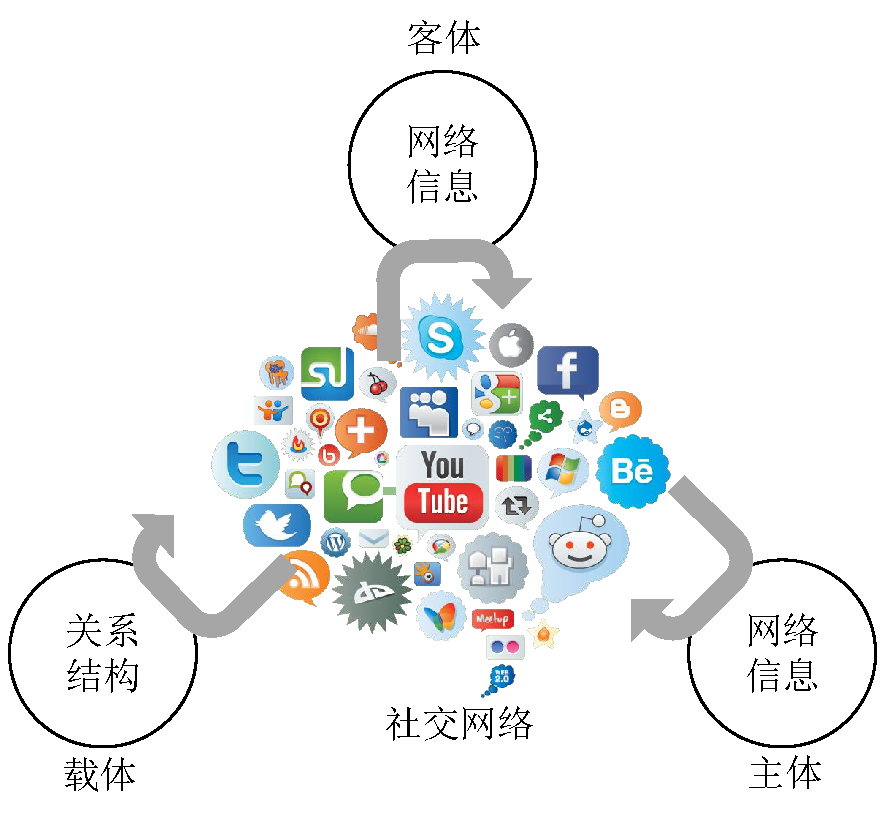
\includegraphics[width=0.5\textwidth]{threeFactors}
    \caption{在线社交网络中的关系结构、网络群体和网络信息}
    \label{fig:threeFactors}
\end{figure}

与传统的Web应用和信息媒体相比,在线社交网络具有如下的新特性:
\begin{itemize}
	\item 高速性:信息发布和接收十分便捷、迅速。社交网络中的用户可以通过手机、笔记本、电脑等终端,随时随地发布和接收信息,信息传递的效率高,具有高速性。
	\item 扩散性:裂变式的信息传播。社交网络中的信息一经发布,便会立刻推送给所有的关注者。信息经过转发,信息又将传播到下一批关注者。信息的传播呈现一种链式反应的几何级数扩散模式,为普通网民传播信息提供了渠道。
	\item 平等性:人人都有可能成为信息输出者。与传统信息媒体中信息发布和信息接收的非对称性相比,社交网络中的每一个参与者都有机会通过社交网络表达自己的观点,传播自己的信息,输出自身的价值观。因此,社交网络在热点事件的产生、发酵、传播等环节中扮演了重要的角色。
	\item 自发性:呈现自媒体形态、自发地形成虚拟社区。社交网络中的个体既是信息的接收者也是信息的发布者,用户会根据自身不同的关注内容与其他用户建立联系,形成网络中的虚拟社区。
\end{itemize}

这些丰富的特性让在线社交网络具有和其他信息媒体不一样的特点,同时也对信息安全提出了新的挑战。对于社交网络分析的研究,在结构、群体以及信息等方面都存在很多已有的工作。其中很多研究工作是关于网络中的信息传播、影响力、传播模型等。这些工作主要研究是否可以建立模型来解释信息的传播方式,如何在真实社交网络信息传播数据集上验证传播模型等等,这些仅仅是社交网络中信息传播研究的一些研究举例。信息传播在实际生活中有着许多应用,例如商业产品或者理念的推广营销、网络流量的爆发检测、寻找关键博客来获取重要的信息、寻找意见领袖或者潮流引领者以及信息的检索排序等等。

社交网络中信息传播关键技术的研究对于理解信息传播的机理有着重要的意义。本文首先在结构上进行理论研究,思考在社交网络中如何选取源节点才能使得信息传播效率更高,提出了传播效率最大化问题。然后,本文在内容方面进行分析,思考社交网络中不同用户的文本内容推送问题。本文利用语言模型以及深度学习等技术,对普通文本信息以及数据流信息进行应用,进行了基于语义扩展和文本质量的实时个性化搜索研究和基于卷积神经网络的文本分类研究,分析不同用户的关注点,将用户所感兴趣的、高质量的信息自动地推送给用户,使得用户更加便捷地获取信息,从而推动信息的传播。最后,本文在传播效果的评估方面进行分析,研究合理的传播模型。本文建立基于概率阅读的传播模型,对于事件的传播影响进行评估,来估测事件传播影响面的大小。本研究对于揭示信息传播的机理和规律、推动社交网络中的信息传播、发现有价值的信息以及保护信息安全起到了重要的作用。

本章首先对本文的研究背景进行阐述,第\ref{sec1:background}小节对在线社交网络中信息传播研究的发展现状进行描述,分析社交网络信息传播分析的研究意义和面临的挑战。其次,第\ref{sec1:relatedWorks}小节对本文研究的各个相关工作进行概述和总结。然后,第\ref{sec1:inovation}小节介绍本文的主要研究内容和创新点。最后,第\ref{sec1:paperStructure}小节给出了本文的组织结构。

\section{研究背景及意义}
\label{sec1:background}
本节主要介绍本文研究的背景及其意义,对涉及到的概念进行详细的阐述,对研究所面临的挑战进行分析。首先,本节对在线社交网络进行一个概述,介绍在线社交网络的起源、定义、特点以及发展状况。其次,本节对社交网络中的信息传播进行介绍,详细地描述信息传播的特点及其所涉及到的因素。然后,本节对本文的研究的意义进行总结。最后,本节分析了研究所面临的挑战。
\subsection{在线社交网络概述}
\label{subsec1:introduction}
人类自诞生以来,就过着群居的生活,一同劳作、交流以及分享,从而形成了社会。随着人类文明的发展和社会的进步,人与人之间的关系进一步的深入和加强,社会关系由简单的血缘关系向朋友关系、雇佣关系以及社交关系发展。而人与人之间由生活、工作、学习、娱乐等等社会交互而形成了某种稳定的关系,这一系列的关系将社会个体结合成了一个巨大的网络,这即是社交网络。如同Linton Freeman所说的那样,我们都被一个无形的网络连接在一起\upcite{freeman2004development}。

社交网络(Social Network)在维基百科中被定义为由社会个体(例如个人或者机构等)、社会个体间的二元关系以及社会个体之间的社交互动组成的社会结构\upcite{social_network}。在社交网络中,个体之间因为社交互动而形成相对稳定的关系体系,这种关系可能是亲属关系、朋友关系、同学关系,也可能是商业合作关系或者宗教信仰关系等。通过这些关系,社交网络把偶然相识的弱关系到紧密结合的强关系,以及社会中各式各样的人群串联成了一张巨大的网络。由于社交网络中存在各种各样的社会关系,个体之间的网络结构往往是非常复杂的。而且,复杂的关系结构也会影响网络中个体之间的社交互动,进而影响到个体的社会行为。

随着工业化、城市化的进行以及移动网络的发展,社会网络化的趋势日益凸显。在2012年,Lee Rainie和Barry Wellman在其著作《网络化:新的社会操作系统》\upcite{rainie2012networked}中指出,社会网络革命、移动革命以及互联网革命将是影响人类社会发展的三大革命。随着互联网的进步,网络结构受地域性因素的影响减弱了,这使得跨地域性的线上社会关系成为了社交网络的主要形式。在现实社会中,人们相继在社交媒体平台上创建账号,将线下的社会关系扩展到了线上,并且进一步的延伸,这使得在线社交网络成为了人们网络生活中不可或缺的沟通工具。

在2009年欧盟关于社会计算的研究报告中\upcite{huijboom2009key},在线社交网络主要可以分成如下的四个大类,
\begin{itemize}
	\item 即时通讯应用。这一类的应用提供一个实时的通信平台,使得人与人之间能够通过网络进行在线的交流、信息的分享等。典型的代表有MSN、QQ、飞信等,其具有双向认证与实时推送的特点。
	\item 在线社交应用。这一类的应用提供一个在线社交关系平台,人们在平台上进行社交互动以及消息的共享等。典型的代表有脸书(Facebook)、谷歌+(Google+)、人人网、QQ空间等,其具有双向认证以及非实时推送的特点。
	\item 微博类型应用。这一类的应用提供一个自媒体的信息发布平台,任何个人或者机构都能在平台上发布信息,推送给其关注者。典型的代表有推特(Twitter)、新浪微博、腾讯微博等,其具有单向认证以及实时推送的特点。
	\item 共享空间以及其他应用。这一类的应用提供一个公告发布系统,具有沟通功能,但是用户之间结合不紧密。典型的代表有BBS、论坛、博客等,其具有单向认证以及非实时推送的特点。
\end{itemize}

社交网络是Web 2.0时代的具有代表性的应用,具备Web 2.0时代交互性、主动性的特点,众多社交软件应用随着技术的更新而蓬勃发展。中国流行的即时通信软件“腾讯QQ”诞生于1999年,在2016年的月活跃账户数(MAU)达到8.77亿,其中智能终端月活跃账户达到6.47亿\upcite{tencentReport2016}。2004年于美国上线的社交网络服务网站脸书(Facebook)成为了全球范围内最流行的社交网站之一。从网站成立至今,其用户持续增长,在2016年第四季度,脸书月活跃人数已经突破了18.6亿,其中移动端用户数达到了17.4亿\upcite{facebookReport2016}。2006年微博客类的应用推特(Twitter)在美国诞生,允许用户更新不超过140个字符的消息,成为一个广受欢迎的社交网络及微博客服务网站。截至2016年第四季度,推特的平均月活跃用户为3.19亿\upcite{twitterReport2016}。随着全球社交网络的发展,相似的网站在国内也纷纷出现。2009年,新浪微博正式上线,政府、明星以及草根用户等社会各界人士纷纷开设账户,发布和接收信息。截至2016年底,新浪微博的月活跃用户数达到了2.97亿,其中89\%的用户为移动端用户,平均日活跃用户(DAU)达到了1.32亿\upcite{weiboReport2016}。腾讯在2011年推出的一个为智能终端提供即时通讯服务的软件“微信”在当今已经成为了新时代移动端即时通讯的领军,微信和WeChat(微信的海外版)在2016年的合并月活跃账户数达到8.46亿\upcite{tencentReport2016}。

随着网络科技和设备产品的飞速发展,社交网络逐渐成为人们接收传播信息、发表自身观点以及讨论公共事件的主要渠道。根据中国互联网络信息中心(CNNIC)发布的第39次《中国互联网络发展状况统计报告》显示,截至2016年底,中国网民的规模达到了7.31亿,与欧洲的人口总量相当,互联网的普及率达到了53.2\%。其中手机网民占比达到了75.1\%,规模达到6.95亿,增长率连续三年超过10\%,移动互联网极大地丰富了网民获取信息的通道\upcite{cnnic2017zghlwfzbg}。随着网民数量的增长,社交网络中的信息量也随之上升。推特中每天产生的信息突破了0.58亿条,查询次数突破了21亿次\upcite{statisticbrain2017twitter}。脸书平均每20分钟就有1百万条链接被分享、3百万条信息发布\upcite{statisticbrain2017facebook}。2017年的春晚直播期间,在新浪微博平台中讨论春晚的微博数量达到了近6千万条,网友互动量达1.99亿次,共有超过1.2亿网友参与到了微博抢红包的活动中\upcite{techsina2017newyear}。2017年的除夕,国人在微信和QQ平台上使用红包互送祝福,其移动支付峰值达到了20.8万笔/秒,合计支付总数达到了32.2亿笔\upcite{techqq2017luckymoney}。由以上数据可以看出,社交网络为人们生活的各方面都提供了平台,成为了人们获取、发布以及传播信息的关键渠道。

社交网络之所以能够如此迅速的流行起来,是因为它具有如下一些特点。首先是社交网络简单易用。任何个人或者组织都能够随时随地发表言论,分享内容。而且,用户接收和发布信息的渠道多种多样,可以在互联网的客户端,也可以在移动客户端。这些都极大地加速用户接收、发布和传播信息的速率,使得信息在群体之间的传播更加的高频化。其次是社交网络交互频繁。社会个体通过关注/被关注、好友等关系紧密联系在一起,网络结构复杂。群体之间通过兴趣爱好、共同关注点等因素形成较为固定的社区,社区内部的成员在同一个话题上相互讨论、分享。与传统信息媒体不同,社交网络中的社会个体既是信息的接收者,又是信息的传播者,同时还可能是信息的传播者。这些因素都促进了社交网络中信息的产生与传播。然后是社交网络与现实社会相互映射。随着社交网络的发展,越来越多的个人和机构在社交网络中实名认证,在网络世界中与人们交互来提高自身的影响力。这进一步地拉近了虚拟和现实之间的差距,真实社会中发生的事件将会迅速的在社交网络中以信息的形式发布与传播。

由于上述的原因,社交网络迅速崛起,在短时间内吸引了大量的用户加入。用户在社交网络中分享现实社会中发生的事件,发表自己的意见,这也使得虚拟网络和现实世界的界线逐渐模糊。由于网络资源的公开性以及透明性,社交网络中的数据相对于现实世界要易于获取,这使得一些原本在现实世界中难以研究的内容存在了研究的可行性。研究者可以分析虚拟网络中的数据,并通过现实世界在虚拟网络中的映射,间接来研究现实世界中的问题。例如人口年龄分布问题、政策满意度问题、舆论热点分析等等都可以在社交网络中得到较好的解决。正因如此,社交网络的出现促进了社会学、传播学、系统科学、计算机科学等学科新一轮的发展。

\subsection{社交网络信息传播}
\label{subsec1:informationDiffusion}
在线社交网络与生俱来的自由性和开放性,使其成为了现代社会中信息传播的重要渠道,社交网络中的信息传播活跃度达到了前所未有的程度。信息传播(Information Diffusion)是指个体、组织之间的信息传递和交流\upcite{baike2017info}。人们通过符号、信号等信息载体来接收、传递与反馈信息的活动,人们相互交换思想和意见等,以达到相互影响和了解的过程。而社交网络信息传播指的是以社交网络为媒介进行信息传播的过程\upcite{方滨兴2014在线社交网络分析}。1948年,Lasswell在《社会传播的结构与功能》\upcite{lasswell1948structure}一文中指出了传播过程及其“5W”要素,即:谁(Who),说了什么(Says What),通过何种渠道(In Which Channel),对谁(To Whom),造成了什么结果(With What Effect)。经典的5W传播模式构成了传播学中研究的五个基本内容,即控制研究、内容分析、媒介研究、受众研究以及效果研究。

社交网络信息传播影响着生活的各方各面,并且改变人们的行为模式。2007年,Christakis和Fowler在新英格兰医学杂志上的发表文章\upcite{christakis2007spread},研究分析了12,000名患者的药物记录,并根据患者之间的亲属关系、邻居关系等,从药物记录中抽取了一个离线的社交网络。研究的目的是分析非传染病(例如肥胖症等)与患者社交网络邻居的关系,理解具有患非传染病网络邻居和自身患有该非传染病的关联关系。在不考虑其他原因的情况下,研究表明拥有肥胖症患者朋友会使得自身也患肥胖症的风险提高171\%。这说明了肥胖症患者会通过社交网络把容易导致肥胖的习惯传播给其网络邻居。该研究主要把重点放在了关联关系上,而不是患病原因,研究结果表明了社交网络间传播影响的效应。在Christakis和Fowler的另一个研究中,吸烟这一个行为也在社交网络中的传播影响也得到了印证\upcite{christakis2008collective}。在2011年,Christakis和Fowler在其著作\upcite{christakis2009connected}中指出了传播的重大影响,并解释了社交网络的组成和运作机理。其中包含了很多真实的案例,例如背痛的症状自柏林墙推倒后从西德传入东德,自杀倾向通过社团传播,政治倾向和信仰通过网络传播等。而在商业圈,信息传播引领成功的最为著名的案例是“Hotmail现象”\upcite{hugo2001emergence}。在20世纪90年代初,Hotmail是一个相对冷门的邮件服务提供商。为了改变这个局面,公司使用了一个相对简单的创意,即在每一封用户发送的邮件结尾自动地加上“欢迎加入世界上最大的邮件服务提供商MSN Hotmail”这一宣传语。这一宣传语通过用户之间的邮件传播,加速了品牌的树立和传播。在短短18个月后,Hotmail就成了世界第一大邮件服务提供商,拥有了800万用户。在2012年7月发布的一首韩国流行歌曲“江南style”成为了YouTube上最先突破10亿观看的节目。而在另一方面,社交网络中的信息传播在社会的突发事件中也有着体现。在2011年夏天,加拿大温哥华举办的史丹利杯冰球决赛引发了骚乱。其中许多是青少年,他们破坏了城镇中的财物,并且在社交媒体上自吹自擂,例如发布图片、视频等。这引发了广泛的传播,并且成为了法庭的取证。相比于现场的证据,社交媒体中的证据种类更多。这使得警方在短时间内确认了骚乱者的身份。

社交网络中的信息传播具有以下特点。首先,社交网络中的信息发布与接收十分便捷、快速,用户可以通过手机等移动设备随时随地发布和接收信息。其次,社交网络中的信息传播的扩散形式呈“裂变式”扩散。消息一经发布将即刻推送到关注者,而关注者的转发将产生下一轮的传播。然后,社交网络中的每一个用户都有成为意见领袖,热点制造者的可能,所有网民都可能在热门事件的传播中扮演重要的角色。最后,社交网络中的信息传播呈现“自媒体性”,任何一个用户或者机构都能够建立属于自己的媒体,通过发布信息、制造热点、传播信息来扩大自身的影响力。这些特点使得社交网络中的信息传播更加迅捷、传播范围更广,人们在社交网络中的交互更加的频繁。

社交网络信息传播之所以有如上的特点是由于如下几个因素\upcite{方滨兴2014在线社交网络分析}。首先是关系结构。社交网络中的个体基于相互认识、兴趣爱好或是个人崇拜等原因,在社交网络上形成了复杂的关系结构。其次是网络群体。基于社交网络中的关系结构,网络个体因为关系而大量聚合,并且相互作用、相互影响,从而形成具有不同特征的网络群体。最后是网络信息。社交网络中的关系结构提供了底层的高速传播通道,网络群体直接助力网络信息的传播,丰富的网络内容提供了信息资源。关系结构、网络群体以及网络信息的有机结合加速了网络信息的传播。

\begin{itemize}
	\item 网络结构。社交网络中的个体间进行丰富的交互,形成了“一对一”、“一对多”、“多对多”以及“多对一”几种传播模式的组合。网络结构中节点间的连接强度和网络密度各不相同,从而形成了不同的连接关系。强连接会导致形成紧密联系、聚集的社区结构,意见更加统一;弱连接通常在关系不紧密、联系不频繁的个体间形成,可以提供新的信息,丰富了信息的内容,扩大了传播范围。
	\item 网络群体。网络个体聚合并且相互影响、形成了网络群体。与现实世界中的群体相比、网络群体传播具有高度的互动性、开放性、跨地域性等特点。网络群体中的意见领袖往往具有较大的影响力,能够引领其所在群体对于事件的倾向性和态度。
	\item 网络信息。网络信息具有时效性、多源性、多样性等特点,在信息传播时起着不可或缺的作用。社交网络的信息的源头不仅仅是网络中的链接信息,而且来自于传统媒体的信息接入。网络信息在社交网络中传播会产生相互影响,与独立信息的传播不同,可能引发更多的讨论和演化。
\end{itemize}

社交网络信息传播由于这些新的因素的出现,凸显出与传统信息传播的不同特性,加速了信息传播的效率和多样化。在实际生活中影响到人们的各方各面,在给人们带来巨大便利的同时,也对信息安全提出了新的挑战。
\subsection{研究意义}
\label{subsec1:researchSignificance}
研究社交网络中信息传播对科学研究、社会安全以及商业发展都是十分有意义的。研究社交网络中的信息传播规律,有助于加深我们对于社交媒体的理解,解释社会中发生的现象,同时使得我们对于复杂的网络拓扑结构、传播能力以及网络动力学等有着进一步的认识。

从科学研究的角度来讲,研究社交网络中的信息传播更有益于理解信息的传播机理,方便推动或者干预信息在人类社会的传播。随着社交网络的发展,各类社交媒体的兴起,用户在网络上发布信息的数量呈爆炸式增长,这些信息通过社交网络这一个良好的渠道在用户之间迅速传播。社会中的事件都会在网络中得到体现,用户将分享个人的生活、讨论热点事件、发表政治观点等等。社交媒体中的信息量已经逐渐超越了传统的新闻、博客等应用的信息量,社交网络成为了信息传播的主要平台。信息在传统的媒体中传播往往通过线上线下的口口相传等途径,而这些方式难以形成记录。社交网络中的信息传播有迹可循,能够记录其传播轨迹,这为开展相关研究提供了丰富的数据基础,使得研究人员有机会在海量的真实数据上建立模型,研究信息传播机制,认识传播规律。

从社会安全的角度来讲,研究社交网络中的信息传播能够使得人们及时接收到真实的信息,免受谣言的危害,保护社会公众的安全与财产。社交网络融入了人们的日常生活,改变了人们的生活方式,影响到包括政治、教育、经济、文化等等方面。在政治方面,微博已经直接在很多政务活动中发挥了巨大的作用。在2008年的美国大选中,奥巴马及其团队利用社交媒体推特进行了助选活动,在推特上制造舆论,争取选票。奥巴马接受竞选总统提名的演讲创下了推特每分钟发表推文5.2万条的记录。在当选之后,奥巴马及其团队继续利用社交网络提高政治影响力。在教育方面,美国的众多大学纷纷在社交网络上发布公开课,直接支持远程教育,并且在脸书和推特上与慕课(MOOC)进行资源整合。在经济方面,电子商务已经成了人们的主流购物方式之一。众多的公司通过社交网络进行宣传,提升自身品牌的竞争力,最终提高了营业额。在文化方面,社交网络正在改变人们的生活方式,足不出户便能与世界各地的网友进行互动,直播平台、虚拟现实技术的诞生使得人们的交互体验更加的多样化。与此同时,社交网络中的信息传播也会给社会带来负面影响。在政治方面,不法分子蓄意制造和传播有害国家安全和社会利益的谣言,影响社会稳定。我们民众曾多次受到微博谣言的影响而发生“抢盐”风波。在教育方面,邪恶势力通过社交网络蛊惑青少年崇尚暴力,灌输错误思想,怂恿其破坏社会的稳定。在经济方面,网络诈骗者利用社交网络发布虚假信息,进行诈骗活动,损害人们的经济利益。在文化方面,犯罪团伙利用社交网络,传播网络色情以及暴力信息,而且往往伴随着传播网络病毒、木马等行为。

在商业发展的角度来讲,研究社交网络中的信息传播能够使得个人、公司或者组织抓住机遇和挑战,实现自身利益的最大化。个人通过社交媒体发布自己的观点、看法,成为社交网络中的意见领袖,形成自媒体。社交网络使得推广自己更加的便捷、简单。例如,罗振宇在社交网络中推广“罗辑思维”节目而走红,成为了自媒体“首富”。而互联网企业通过分析社交网络中的趋势,制定自身的战略方向,通过社交网络发布自己的产品或者理念,能够快速地推广自身的产品。同时,社交网络中的个人信息透明化,使得个人隐私更容易被利用,这对隐私保护提出了新的要求。社交网络中信息传播速率快,传播范围广,这对企业的公关能力提出了挑战。

综上所述,社交网络的发展对社会各方各面都带来了机遇和挑战,同时也对人们提出了新的要求。研究社交网络信息传播有助于理解传播的机理,提高应对突发事件的能力,促进经济的繁荣发展,对于政治经济安全、国家社会稳定以及企业个人财产利益都有着重要的意义。
\subsection{面临的挑战}
\label{subsec1:challenge}
在线社交网络中信息传播分析与自然语言处理、数据挖掘、机器学习、海量数据处理、传播学、社会学等等学科有着紧密的联系。社交网络带来了丰富的语料数据和结构关系,但是也提出了新的挑战。尽管与之相关的各个领域的研究已经取得了很多的成果,提供了相应的技术支持。但是,由于在线社交网络中的信息传播同以往的研究存在诸多不同之处,这一研究依然面临着新的问题与挑战,具体包括如下几个方面。

\begin{itemize}
	\item 数据的海量性。社交网络信息传播分析所涉及到的数据量往往是海量的,这对信息传播的分析提出了较大的挑战。数据的海量性体现在两个方面,一个是信息内容海量,二是用户结构海量。这对信息传播的分析算法处理数据的能力提出了新的要求。在一些热点突发事件的爆发过程中,社交网络中的信息往往在短时间内便会达到一个较大的数量级,例如2016年奥运会中的中国女排夺冠,“女排精神”成为了国人共同的关注点,女排夺冠相关内容互动量在当天达到了7285万次,相关视频播放量达到3.4亿次\upcite{sina2016volleyball}。信息传播分析通常需要分析文本的内容,分析用户之间的传播关系等,如何实时地处理如此庞大的数据是社交网络信息传播需要研究的问题。
	\item 文本的多样性。社交网络中的文本形式多样,微博类的应用通常限定用户的文本长度不超过140个字符。而新闻、论坛或者微博中的长博文则对用户发表文本的长度没有严格的限制。这使得传统的文本表示模型在社交网络中,对长短文本的处理性能明显下降,在文本分类、文本聚类、信息推荐等应用方面影响较大。因此,社交网络中的信息该如何表示对社交网络中信息检索、信息推荐等应用提出了新的挑战。
	\item 结构的复杂性。社交网络中的用户数量庞大,而且不同社交媒体之间的用户存在着重叠现象。社交网络中的用户通过朋友、兴趣等多种关系聚合在一起,形成多种多样的复杂结构。计算信息传播的影响范围、信息的溯源以及如何选择节点使得影响力最大化这些问题在社交网络环境中都出现了新的挑战,传统的方法的性能在复杂的网络中效率明显下降。如何在复杂的网络中快速地、有效地对信息传播进行分析对抽样理论、算法设计等都提出了挑战。
\end{itemize}

由此可见,社交网络的发展对信息传播研究提出了多方面的挑战,同时,也为信息传播研究提供了丰富的数据和渠道,这也为信息传播的研究提供了一个虚拟的环境。

\section{相关研究工作}
\label{sec1:relatedWorks}
社交网络中的信息传播相关的工作涉及到的研究十分广泛,包括自然语言处理、数据挖掘以及机器学习的各种研究方法。本小节主要从传播源的选择、信息内容的选择以及传播效果的评估等方面介绍相关的研究工作。其中涉及到的相关工作有影响力最大化、实时个性搜索、语言模型与文本分类以及传播模型的学习等相关研究。
\subsection{影响力最大化}
\label{subsec1:influenceMax}
影响力最大化问题的实际应用是通过信息传播来推广新产品、新理念以及新政策等。为了实现网络中信息的迅速传播,主要有研究分为两个方向。第一个方向是传播模型的建模,第二个方向是寻找一个快速有效的方法来找到具有影响力的个体。

对于第一个方向,已有很多工作对传播模型进行了深入的研究。均匀模型(Uniform Model)假设所有节点的影响概率为一个常数(例如0.01),该模型不区分节点之间的关系。首先,每一个节点都以相同的概率影响其邻居节点,模型未能区分节点对于其他节点的影响力。其次,每一个节点受到其邻居节点的概率也是相同的,模型未能区分不同邻居节点对该节点的影响力。显然,这样的假设是值得商榷的。三态模型( Trivalency Model)在一定程度上解决了第一个问题,节点的影响概率为一个集合中的某一个元素,例如$\left\{ 0.001, 0.01, 0.1\right\}$。模型的思想是对不同影响力的节点赋予不同的影响概率值。上述的两个模型的影响概率与网络的结构无关。在加权级联模型(Weighted Cascade Model)中,模型定义影响概率与网络的边$\left(u,v\right)$相关,影响概率$p_{uv}=1/d_{in}v$,其中$d_{in}v$为节点$v$的入度。该模型比均匀模型和三态模型拥有更好的性质。首先,低入度的节点受到其入度邻居节点的影响要大于高入度的节点。这样影响概率不仅仅是从一组常数中进行选择。其次,一个节点对于出度节点的影响不再是相同的,这是由于这些出度节点的入度不同。然而,加权级联模型仍然无法解释节点之间的影响概率是如何计算得出的。Saito等人\upcite{saito2008prediction}研究了如何学习影响概率的问题,主要以独立几联模型为研究对象。通过观测信息传播过程中的每个时间段,来求解设定影响概率为参数下的极大似然估计,从而求解影响概率。在线性阈值模型中,每个节点存在一个阈值$\theta \in \left[ 0,1 \right]$,当累计影响超过阈值时,节点将被激活。Goyal等人\upcite{goyal2010learning}通过社交网络中的信息传播轨迹来学习节点之间的影响概率。

对于第二个方向,影响力最大化问题最早是由Domingos和Richardson所提出,问题基于马尔科夫随机场(Markov Random Field)进行建模\upcite{domingos2001mining,richardson2002mining}。随后,Kempe等人将影响力最大化问题建模成一个离散的随机优化问题\upcite{kempe2003maximizing}。影响力最大化的问题可以定义为如下所示,

\begin{defn}[影响力最大化问题]
\label{def:imProblem}
影响力最大化问题可以形式化为如下一个随机优化问题:给定一个图$\mathcal{G} = \left(\mathcal{V}, \mathcal{E}\right)$、图$\mathcal{G}$上的一个随机传播模型以及一个阈值$k$。给定一个种子节点集合$S \subseteq \mathcal{V}$且满足$\left\vert{S}\right\vert \leq k$,则集合$S$的影响力期望为$\mathbb{E}_\mathcal{G}\left[I\left(S\right)\right]$。则影响力最大化问题为寻找使得影响力期望最大的集合$S^{\ast}$。问题可表示为如下所示,
\begin{equation}
\label{eq:imProblem}
    \begin{split}
        &S^{\ast} = \arg\max{\mathbb{E}_\mathcal{G}\left[I\left(S\right)\right]}\\
        &s.t.~~S \subseteq \mathcal{V},\left\vert{S}\right\vert \leq k
    \end{split}
\end{equation}
\end{defn}

在给定了一个传播模型后,例如独立级联模型(Independent Cascade Model)或者线性阈值模型(Linear Threshold Model),影响力最大化问题可以分解成两个问题。第一个问题称为影响力期望计算问题,即给定了一个种子节点集合$S$后计算其影响力期望$\mathbb{E}_\mathcal{G}\left[I\left(S\right)\right]$。第二个问题是如同定义\ref{def:imProblem}所示,找到使得影响力期望最大的种子节点集合。

对于影响力期望计算问题,Wang等人\upcite{wang2012scalable}以及Chen等人\upcite{chen2010scalableLT}证明了其复杂度在独立级联模型和线性阈值模型下是\#P-难的。\#P问题是计数问题,与NP问题中决策问题相关。NP问题需要求解一个问题实例是否存在解,例如合取范式(Conjunctive Normal Form)方程是否存在可满足解,而\#P问题需要求解这个问题实例存在多少个解,例如合取范式方程存在多少个可满足解。如果一个问题是\#P的且每一个\#P的问题都可以在多项式时间内归约到它,那么这个问题是\#P-完全的。如果一个问题可以在多项式时间内由一个\#P-完全的问题归约到它,那么它是一个\#P-难的问题。对于独立级联模型或者线性阈值模型,上述的证明过程都可以由一个\#P-完全的问题,$s$-$t$连通性问题\upcite{valiant1979complexity},来进行归约。

对于寻找影响力期望最大的种子节点集合的问题,Kempe等人\upcite{kempe2003maximizing}给出了结论,问题的复杂性在独立级联模型和线性阈值模型下都是NP-难的。其证明思路将NP-完全的问题归约到影响力最大化问题。在独立级联模型中,证明将子集覆盖(Set Cover)问题归约到影响力最大化问题;而在线性阈值模型中,证明将节点覆盖(Vertex Cover)问题归约到影响力最大化问题。

上述研究表明了影响力最大化问题是一个复杂性较高的问题。问题的难度来自于两方面,一方面是问题的组合性质,另一方面是计算影响力期望的难度(甚至是计算一个节点的影响力期望)。针对这两个问题,已有的研究主要应用贪心算法来解决组合问题,利用蒙特卡罗(Monte Carlo)模拟来解决影响力期望计算问题。对于影响力最大化问题使用贪心算法能够得到一个下界的保证,即运用贪心算法得到的解最差的结果有理论性的保证。这是由于影响力期望函数$\mathbb{E}_\mathcal{G}\left[I\left(\cdot\right)\right]$具有两个很重要的性质,即子模性(submodularity)和单调性(monotonicity)。子模性的定义如下所示,
\begin{defn}[子模性]
\label{def:submodularity}
子模性的定义可以解释为往种子节点集合加入更多节点时,所造成的效果为边际收益递减(Diminishing Marginal Returns)。对于一个集合函数$f:2^{\mathcal{V}} \rightarrow \mathbb{R}$,如果对于任意的子集$S \subseteq W \subseteq \mathcal{V}$且任意的元素$v \in \mathcal{V} \setminus W$,将元素$v$加入到集合$W$中的边际收益不超过将元素$v$加入到集合$S$中的边际收益,那么函数$f\left( \cdot \right)$具有子模性,用公式表示如下,
\begin{equation}
\label{eq:submodularity}
	f\left(S\cup\left\{v\right\}\right) - f\left(S\right) \geq f\left(W\cup\left\{v\right\}\right) - f\left(W\right)
\end{equation}
\end{defn}

另一个重要的性质单调性定义如下,
\begin{defn}[单调性]
\label{def:monotonicity}
单调性的定义可以解释为往集合中增加元素不会使得函数值变小。一个集合函数$f:2^{\mathcal{V}} \rightarrow \mathbb{R}$,如果对于任意的子集$S \subseteq W \subseteq \mathcal{V}$,都有$f\left(S\right) \leq f\left(W\right)$,则函数$f\left( \cdot \right)$具有单调性。
\end{defn}

对于具有子模性和单调性的函数$f\left( \cdot \right)$,Nemhauser等人\upcite{nemhauser1978analysis}证明了使用贪心算法得到的解的性能存在着下界。令$S^{\ast}$表示问题的最优解,函数$f\left( \cdot \right)$具有子模性和单调性且满足$f\left( \emptyset \right) = 0$,$S^g$为通过贪心算法得出的解,则可以用公式表示为如下所示,
\begin{equation}
\label{eq:lowerBound}
	f\left( S^g \right) \geq \left( 1 - 1/\mathsf{e} \right) f\left( S^{\ast} \right)
\end{equation}
其中$\mathsf{e}$为自然对数的底。其证明过程\upcite{chen2013information}利用了单调性和子模性以及递推方法得到公式(\ref{eq:lowerBound})的结论。

对于影响力最大化的求解,Kempe等人\upcite{kempe2003maximizing}的研究是最早将影响力最大化问题当做优化问题来求解的,并且给出了贪心算法的求解。Leskovec等人\upcite{leskovec2007cost}提出了一种改进算法,CELF算法。算法利用函数的子模性来对于不必要的模拟进行剪枝,使用一个优先队列实现,在不改变输出的情况下提高了算法的性能。Goyal等人\upcite{goyal2011celf++}基于上述的工作进行了改进,提出了CELF++算法。Cheng等人为了解决可扩展性和准确度之间的矛盾,提出了一个静态的贪心算法,为StaticGreedy算法。该算法保证了信息传播过程中影响函数的子模性,在准确度不损失的情况下,极大地降低了运算量。Borgs等人提出了一种不同于贪心算法的新型框架,利用了反向传播抽样方法,极大地加速了算法的效率,同时保证了算法的性能。

基于影响力最大化问题,许多研究提出了基于此之上的衍生问题。传统的影响力最大化问题是种子节点集合的大小进行限制,阈值为$k$。Leskovec等人\upcite{leskovec2007cost}假设选择每一个节点都会产生开销,每一个节点的开销不尽相同,而总开销的大小固定作为限制,问题是在不超过总的预算下来产生最大的影响。在某些情况下,网络可能是动态的网络,在动态网络中研究影响力最大化问题\upcite{chen2015influential,zhuang2013influence}也是一个十分有意义的方向。Yang等人\upcite{yang2016continuous}对动态的影响力最大化问题进行研究,提出了一种通用的坐标下降算法来解决该问题。Wang等人\upcite{wang2015maximizing}在原问题的基础上,考虑了激活的节点以及最终传播到单未激活的节点(称之为已通知的节点)两类节点,提出了信息覆盖最大化问题(Information Coverage Maximization),并对该问题进行了求解。Liu等人\upcite{liu2012time}将传播时间纳入了考虑,提出了一种时间约束的影响力最大化问题。Shishir等人\upcite{bharathi2007competitive}考虑到了信息传播中多个传播源博弈游戏,对多源情况下的信息竞争传播问题进行了分析,对先手情况给出了求解方法。

\subsection{实时个性化搜索}
\label{subsec1:realTimeSearch}
实时个性化搜索的目的是根据用户偏好迅速地识别出用户所感兴趣的物品或者内容,涉及到许多的研究领域,包括个性化搜索、语言模型以及协同过滤等等。

在个性化搜索方面,根据不同的用户,对于检索内容进行重新排序是提高性能的一个常用的方法。Xie等人\upcite{xie2016personalized}针对上下文关系中的语言知识,使用图结构对语言知识的内容和相互关系建模,从而获取用户的偏好。同时,该工作提出了一个发现支配集的算法,来降低非相关上下文的影响,并提出了一个重排算法来衡量一次查询与信息的相关性、发现的文本内容与用户信息的相关性。Sontag等人\upcite{sontag2012probabilistic}针对特定用户的个性化搜索提出了一个新的方法。工作提出了一个关联生成模型,可以用来针对一次查询计算文本和用户的关联。生成模型中的用户相关的参数构成了一个用户的信息,可以通过用户长期的搜索记录来进行学习。Wang等人\upcite{wang2013personalized}针对搜索引擎对用户不区分的问题,提出了一种通用排序模型的适应性框架来解决个性化搜索问题。模型使用一个离线训练的用户无关的排序模型以及有限数量的不同用户的查询,能够更好的适应不同用户的搜索偏好。Tang等人\upcite{tang2015personalized}将个性化推荐问题形式化为一个上下文歹徒问题(\textit{contextual bandit problem}),来解决获取新的知识和基于已有知识做决策的相互制约问题。工作提出了一种非参数的策略,使用了一个有规则的重采样方法来得到需要估测模型的分布。根据概率匹配的模式,算法随机地从得到的分布中选取一个模型。Leginus等人\upcite{leginus2016personalized}针对推特中信息量繁多,而用户无法处理大量信息的问题,提出了个性词语云生成的方法来作为用户导航。用户的行为历史,例如发布的推文、转推、浏览的推文,都可用来提升词语云的个性化。Du等人\upcite{du2016folksonomy}对协同标签系统中个性化搜索中的用户建模进行了研究,通过标签以及排序等信息,提出了一种多层次的用户模型,实现个性化搜索。模型不仅能够反应出用户的偏好,也能反应出用户不喜欢的内容。Younus等人\upcite{younus2014language}针对个性化搜索引擎中的用户模型进行了研究,利用推特作为个性化搜索引擎的用户信息源,提出了一种统计语言模型,将推特中的用户特征考虑在内。个人化的用户模型使得检索的准确率得到了显著的提高。Xie等人\upcite{xie2014mining}针对社交网络中隐藏用户社区发现问题进行了研究,提出了增强分类图(Augmented Folksonomy Graph)的机制来包含社交网络中的多方面关系,同时基于一种新型的密度估计的聚类方法来寻找隐藏的用户社区。Li等人\upcite{li2015real}针对社交网络中的频繁信息更新以及小世界特性,提出了一种通用框架来解决个性化top-k查询问题。框架基于通用的排序框架,集成了时间新鲜度、社交相关性以及文本相似度特征。算法应用了一个三维立方倒排索引来支持在三个特征维度上有效的剪枝。然后提出了一个基于该立方的算法来检索top-k的结果。

在短文本的研究方面,由于社交网络中的文本具有不同的性质,包含了更多的标签以及结构化和非结构化的属性,因此对这方面的研究是十分有必要的。在社交网络中的信息检索方面,Massoudi等人\upcite{massoudi2011incorporating}为了解决社交网络中短文本信息量不足的问题,提出了一种检索模型,对特定话题检索微博中的博文信息。由于传统的信息检索模型在微博中无法直接适用,研究针对微博的特性设计了一种语言模型。算法通过文本特性和微博特性两方面对模型的性能进行提升,同时使用了一个动态的查询扩展模型来对微博博文检索进行处理。Severyn等人\upcite{severyn2015learning}使用了卷积神经网络来重排短文本对(查询-文档对),其中神经网络可以用来表示短文本对以及计算他们之间的相似度。该算法将词语当做输入,简化了预处理过程。该方法在TREC的两个常见的任务(智能问答以及微博检索)中显示了较好的性能。Ren等人\upcite{ren2014hierarchical}在社交网络流数据中的层次多标签的分类中进行了研究,由于概念漂移、种类之间的复杂关系以及社交网络数据流中的文本长度有限对该问题都提出了挑战。研究的核心思想包括短文本的扩展、时间感知的话题追踪和基于块结构的学习。Paik\upcite{paik2013novel}对信息检索中的词语权重问题进行了研究,提出了一种新型的tf-idf词语权重方法。算法使用了两种不同的文档词频归一化来得到两方面的词语特性。一种词频在短文本中效果较好,另一种在长文本中效果较好,最终的词语权重综合考虑了这两部分的影响。

在协同过滤搜索方面,由于社交网络中的信息和用户紧密相连,优质的用户更可能产生有意义的信息。Xue等人\upcite{xue2009user}针对传统搜索中两个主要问题,数据稀疏性以及新用户的冷启动,提出了协同个性化搜索的方法。该方法不仅考虑了特定用户群和全局用户之间的共性,并且考虑了个体的特性。方法建立一个统计用户语言模型来结合个人模型,用户群模型以及全局用户模型。Vosecky等人\upcite{vosecky2014collaborative}针对微博领域内协同搜索的不足,针对推特中的协同个性化搜索提出了一种新型的框架。算法的核心是一个协同用户模型,该模型用来表示用户的社交连接,从而获取用户更全面的偏好。

\subsection{语言模型与文本分类}
\label{subsec1:textClassification}
语言模型是研究文本的基础,包括特征提取、特征权重以及语义相似度计算等。特征提取研究的是选取哪些特征来表示文本的问题,特征权重以及语义相似度计算则是计算问题。特征选择存在许多不同的方法,可以采用词语、短语等作为特征,也可以采用n-gram模型选择特征项,也可以采用知识库中的概念作为特征项。

布尔模型\upcite{salton1975vector}是在文本信息检索中的一种简单的模式,该模型是特征项的严格匹配。每一个特征项的取值都有True和False两种取值,其中True表示文本中存在该特征,False表示不存在。用户的查询采用逻辑运算来表示特征项之间的关系,文本的匹配查询过程则是布尔逻辑运算。该模型的优点是运算速度快,可以表示一定的逻辑关系。但是该模型也存在明显的缺陷,首先是无法对特征值的重要性进行赋值,且缺乏定量的分析。用户在进行查询的时候需要自己构建复杂的查询表达式。查询的结果仅有命中和不命中两种结果,适用范围较小。

向量空间模型(Vector Space Model)是另一种类型的模型。在这个模型中,特征项是代表着向量空间中不同的维度,文本则可表示为该空间中的一个向量,向量中每一个维度的分量可以使用词频、tf-idf值等。例如选择tf-idf值作为分量时,一篇文档$\mathbf{d} \in \mathbf{D}$可以表示为如下,
\begin{equation}
\label{eq:documentVec}
	\mathbf{d} = \left({tfidf}_{1,\mathbf{d}}, {tfidf}_{2,\mathbf{d}}, \cdots, {tfidf}_{N,\mathbf{d}}\right)
\end{equation}
其中${tfidf}_{i,\mathbf{d}}$表示特征项$i$的tf-idf值,$N$为特征的总数。tf-idf值的计算公式如下所示,
\begin{equation}
\label{eq:tfidfFormula}
	{tfidf}_{i,\mathbf{d}} = {tf}_{i,\mathbf{d}} \cdot {idf}_i = \frac{n_{i,\mathbf{d}}}{\sum_j n_{j,\mathbf{d}}} \cdot \log{\frac{|D|}{1 + \vert \{\mathbf{d} \in \mathbf{D} : i \in \mathbf{d}\}\vert}} 
\end{equation}
其中${tf}_{i,\mathbf{d}}$表示特征$i$在文档$\mathbf{d}$中的频率,${idf}_i$表示特征$i$的逆向文件频率,$n_{i,\mathbf{d}}$表示特征$i$在文档$\mathbf{d}$中出现的频数。给定一个文档集合后,每一个文档都可表示成一个向量,则两个文档的相似度计算可以计算向量的余弦相似度,如下所示,
\begin{equation}
\label{eq:cosSim}
	\cos \left( \mathbf{d_1}, \mathbf{d_2} \right) = \frac{\mathbf{d_1} \cdot \mathbf{d_2}}{\| \mathbf{d_1} \| \cdot \| \mathbf{d_2} \|}
\end{equation}
其中$\| \mathbf{d_1} \|$表示文档向量的长度。基于向量空间,还有很多相似度计算方式,包括欧氏距离、曼哈顿距离以及杰卡德相似度等。

自然语言处理中最直观的词表示模型为独热码表示(One-hot Representation)模型,这种方法把每一个词语表示成一个长向量。向量的维度为词语的总数大小,其中只有一个维度的值为1,其余的维度的分量为0。很显然,这种表示模型存在着不足,任意的两个不同的词语之间都是孤立的。为了解决该问题,最早由Hinton\upcite{hinton1986learning}提出分布式表示(Distributed Representation)模型。其基本思想是通过训练将每一个词语映射成一个N维的实数向量(N一般为指定的一个常数)。经过映射后,我们可以通过词语之间的距离(例如余弦相似度、欧氏距离)来判断词语之间的语义相似度。该研究使得语义上相关或者相似的词语,在距离上更加接近。Bengio等人\upcite{bengio2003neural}使用了一个三层的神经网络来构造语言模型来进行语言模型的训练,通过求解带参数的极大似然估计得到一个好的模型。Bengio在APNews数据集上做的对比实验表明了他的模型效果,相比与普通的n-gram算法提升了10\%-20\%。由Michael Collins提出的Log-Linear模型是word2vec所用模型的前身,基于此之上,Mnih和Hinton\upcite{mnih2007three}提出了Log-Bilinear模型,与Log-Linear模型的不同之处在于映射函数部分。同时,Mnih和Hinton\upcite{mnih2007three}进一步结合Morin和Bengio所提出的层次化概率语言模型\upcite{morin2005hierarchical},提出了层次化的Log-Bilinear模型。Mikolov等人\upcite{mikolov2013distributed}基于之前的工作实现了word2vec工具,所提出新的Log-Bilinear模型包括连续词袋模型(Continuous	Bag-of-Words	Model)和skip-gram两种。

为了解决文本的表示问题,已有许多研究对该领域进行了深入的研究。字符串匹配、n-gram模型以及深度学习技术都被用来增强分词的性能。基于n-gram模型的字符串匹配是比较常见的方法,而基于深度学习的方法取得了更好的效果。Zheng等人\upcite{zheng2013deep}针对中文分词问题,使用大规模无标签的数据来增强中文字符的内部表示,然后用来提高表示能力,增强有监督学习中的中文分词性能。Pei\upcite{pei2014max}等人提出了一个神经网络模型,最大边际张量神经网络(Max-Margin Tensor Neural Network)来解决中文分词问题,模型能够处理标签与文本字符间复杂的内在联系。基于循环神经网络(Recurrent Neural Network)的语言模型\upcite{mikolov2010recurrent}有着不错的性能,但是由于反向传播问题而难以进行训练。LSTM(Long Short-Term Memory)是一种特殊的循环神经网络来避免训练过程中的梯度消失问题。由于短文本提供的词语量较少,传统的词袋模型的实用性下降,Sriram等人\upcite{sriram2010short}提出了使用从用户信息中提取出的领域相关的特征,来将文本分类到预定义的类别中。

在文本的多标签分类问题也存在很多已有的研究。Hong等人\upcite{hong2014mixtures}提出了一种基于混合专家框架的概率模型来解决多标签分类问题,该模型结合了条件树结构的贝叶斯网络。Ai等人\upcite{ai2015best}提出了多标签最佳初次过采样(MultiLabel Best First
Over-sampling)的方法来提高多标签分类的性能,方法基于不平衡的最小化求解。为了解决文本分类中测试数据集与训练数据集生成时间不同的问题,Fukumoto等人\upcite{fukumoto2013timeline}提出了一种时间轴自适应的方法。Xu等人\upcite{xu2013uncovering}提出了一种基于KNN和图结构的分类方法来判别电影评论网站中的垃圾用户。

在应用神经网络进行文本分类的工作方面,深度学习在文本分类方面取得了很多成果。Kim\upcite{kim2014convolutional}使用卷积神经网络对语句进行分类,使用预先训练好的词向量作为输入,与多个基准算法进行了对比,取得了很好的效果。Graves等人\upcite{graves2013speech}利用LSTM对语音识别进行了应用,结合了多层次的语音表示进行模型训练,在TIMIT数据集上实现了一个错误率为17.7\%的效果。Iyyer等人\upcite{iyyer2014political}使用了一个循环神经网络结构来对文本中的政治倾向性做判别,算法不仅考虑语义内容而且考虑了句法结构。Kalchbrenner等人\upcite{kalchbrenner2013recurrent}介绍了一个同时面向语句和段落的分类算法,算法结合了卷积神经网络和循环神经网络。同时Kalchbrenner等人\upcite{kalchbrenner2014convolutional}提出了动态卷积神经网络(Dynamic Convolutional Neural Network)的思想,网络采用一个动态的池化层,在智能问答方面的取得了较好的效果。
\subsection{传播模型的学习}
\label{subsec1:diffusionModel}
社交网络中的信息传播或是影响力传播都是按照一个离散的时间段来进行的,例如在时刻$t = 0, 1, 2, ...$。每一个节点$v \in \mathcal{V}$都有两个可能的状态,激活与未激活状态。直观上来说,我们可以认为激活的节点是接收到了信息、是认同了某种观点或是新的产品在网络中进行了传播,而未激活的节点则表示相反的情况。令$S_t \subseteq \mathcal{V}$表示在$t$时刻激活的节点集合,则$S_0$表示种子节点集合,表示信息传播过程中初始激活的节点。这些节点是信息传播过程中被选中来进行传播的节点,例如在商业促销活动中被选中来试用免费样品的用户。

在信息传播过程中,随着时间的变化,激活节点集合是单调非递减的,且节点集合的大小决定了其上限。因此,在有限的时间段后,激活节点集合将不再变化,传播过程结束。令最终稳态的激活节点集合为$\Phi \left(S_0\right)$,其中$S_0$为初始种子节点集合。由于传播过程是个随机的,$\Phi \left(S_0\right)$也是一个随机集合。因此,研究传播模型的重点则在于研究最终稳态激活节点集合的期望$\mathbb{E} \left[ | \Phi \left(S_0\right) | \right]$。目前应用最广、最流行的传播模型包含如下两种,独立级联模型和线性阈值模型,这两种模型首先都是在数理社会学中进行研究。

独立级联模型的当前形式是Kempe等人\upcite{kempe2003maximizing}率先提出的,模型基于相互作用粒子系统中的模型\upcite{durrett1988lecture,liggett2012interacting}以及市场研究的相关工作\upcite{goldenberg2001talk,goldenberg2001using}。同时,独立级联模型与传染病模型\upcite{anderson1992infectious}也是相关的。独立级联模型的核心特点是在传播过程中,社交网络图中每一条边是相互独立的。在独立级联模型中,网络中每一条边$e_{u,v} \in \mathcal{E}$与传播概率$p_{u,v} \in \left[0,1\right]$相关联,表示着节点$u$影响$v$的程度。对于不连接的边$e_{u,v} \notin \mathcal{E}$,传播概率$p_{u,v} = 0$。在下面的定义中,我们定义$S_{-1} = \emptyset$,意味着在加入种子节点前,网络中没有被激活的节点。

\begin{defn}[独立级联模型]
\label{def:icModel}
独立级联模型以$\mathcal{G} = \left(\mathcal{V}, \mathcal{E}\right)$代表网络,传播概率函数$p\left( \cdot \right)$作用于每一条边$e_{u,v} \in \mathcal{E}$。初始种子节点集合$S_0$作为输入,按照如下的规则来生成所有时刻$t \geq 1$对应的激活节点集合$S_t$。对于任意一个时间段$t \geq 1$,集合$S_t$前一时刻的集合为$S_{t-1}$。对于所有在$t-1$时刻未激活的节点$v \notin S_{t-1}$,所有节点$u \in N^{in}\left(v\right) \cap \left(S_{t-1} \setminus S_{t-2} \right)$,即所有在$t-1$时刻激活的节点将尝试去激活其出度节点。节点$u$将进行一次成功概率为$p_{u,v}$的伯努利实验(抛掷一枚独立的硬币)。如果成功,则将节点$v$加入集合$S_t$,并称节点$u$在时刻$t$激活节点$v$。如果有多个节点在时刻$t$激活了$v$,最终的结果是相同的,即将节点$v$加入集合$S_t$。
\end{defn}

根据独立级联模型的性质,该模型适合对信息传播或者病毒传播进行建模。在这些场景下,只需要一个源节点就能使得节点被激活(接受信息或者感染病毒)。社会学家Centola和Macy\upcite{centola2007complex}将这种传播行为称之为简单蔓延(Simple Contagion)。

独立级联模型能够适应于单源激活的传播过程,但是在一些情况下,节点被激活需要收到多源的影响才能改变节点的状态。例如,接受一个为证明的新技术、采纳一个有争议的想法、使用一个昂贵的新产品。在这些时候,人们在决策之前往往需要从多个其他独立的源头获取参考意见。

社会学家首先提出了线性阈值模型\upcite{granovetter1978threshold,thomas1978micromotives}来对此类传播进行建模。当节点受到的正向累积效应(计数、加和等)超过了一定的阈值时,该节点将被激活。社会学家Centola和Macy\upcite{centola2007complex}将这种受到两个或者多个源节点激活的传播行为称之为复杂蔓延(Complex Contagion)。

线性阈值模型作为一种传播模型首先由Kempe等人\upcite{kempe2003maximizing}形式化的提出,并对该模型的性质进行了描述。在线性阈值模型中,网络中的每一条边$e_{u,v} \in \mathcal{E}$与影响权重$w_{u,v} \in \left[0,1\right]$相关联,表示这节点$u$对节点$v$的影响程度。对于某一个节点$v$,影响权重是一个归一化的参数,满足$\sum_{u \in N^{in}} w_{u,v} \leq 1$。对于不连接的边$e_{u,v} \notin \mathcal{E}$,令影响权重$w_{u,v} = 0$。

\begin{defn}[线性阈值模型]
\label{def:ltModel}
线性阈值模型以$\mathcal{G} = \left(\mathcal{V}, \mathcal{E}\right)$代表网络,影响权重函数$w\left( \cdot \right)$作用于每一条边$e_{u,v} \in \mathcal{E}$。初始种子节点集合$S_0$作为输入,按照如下的规则来生成所有时刻$t \geq 1$对应的激活节点集合$S_t$。传播开始时,每一个节点$v \in \mathcal{V}$独立地选择一个阈值$\theta_v \in \left[0,1\right]$,阈值分布服从均匀分布。在任意时间段$t \geq 1$,集合$S_t$前一时刻的集合为$S_{t-1}$。对于所有在$t-1$时刻未激活的节点$v \notin S_{t-1}$,如果它的入度节点累积的影响权重等于或者超过$\theta_v$,即$\sum_{u \in S_{t-1} \cap N^{in}\left(v\right)} w\left(u,v\right) \geq \theta_v$,则将节点$v$加入到$S_t$中,这代表着节点$v$在时刻$t$被激活。
\end{defn}

线性阈值模型中的阈值$\theta_v$表示着节点$v$被激活节点影响的可能性。较大的阈值意味着节点需要更多的节点来激活,较小的阈值意味着节点容易被较少的节点所激活。节点的阈值从0到1随机选择,这反映了对于单独节点内部阈值信息的缺乏。阈值的选择是传播过程中的唯一的随机步骤,一旦阈值是确定的,那么传播过程都是确定的,即每一时刻被激活的节点以及最终激活节点集合。每条边的影响权重$w_{u,v}$反映了节点$u$对于$v$的影响程度,如果$w_{u,v}$较大,且节点$u$已经被激活,则节点$v$更可能会被激活。该模型下允许节点的所有入度边的影响权重和小于1。如果随机生成的阈值$\theta_v$大于所有入度边的影响权重和,则即使当节点$v$的所有入度节点都被激活,节点$v$仍然不会被激活。
\section{本文的工作与创新}
\label{sec1:inovation}
通过对社交网络的新功能、新特性以及带来的新问题、新挑战的分析,基于已有的相关工作的总结,结合计算机科学、传播学、心理学等学科的研究,本论文以信息传播为中心,从影响力最大化、数据流实时推送、社交网络文本分类和传播模型学习四个方面进行研究。

首先在影响力最大化方面,针对传统影响力最大化问题没有考虑到传播时延的缺陷,定义了传播效率函数,提出了传播效率最大化问题,并进行了问题分析,最后应用反向效率采样的方法进行了解决。其次,本文面对社交网络数据流的实时个性化搜索问题进行了研究,结合TREC2015测评的任务,提出了一种结合语义扩展和质量模型的实时个性化搜索框架,为社交网络中数据流的信息个性化推荐提供了支持。然后,结合深度学习在自然语言处理上的应用,本文提出了一种采用卷积神经网络的文本分类方法,同时应用了关键语句的判断,降低了运算的复杂度。最后,本文结合社交网络中的实际情况,以事件为粒度,对事件的影响力量化问题进行分析。研究基于独立级联模型,考虑了多源信息的融合去重、垃圾用户的过滤以及概率阅读因素,为事件的影响力量化分析提供了更准确的方法。

本文的主要工作和创新如下所示:
\begin{enumerate}
	\item 影响力最大化:社交网络中传播效率最大化问题。传统的影响力最大化问题只考虑了最终传播能够影响到的范围,没有考虑到节点需要经历多长的时间段才能被激活,即没有考虑传播的效率。针对这个缺陷与不足,我们提出了一个新的问题,即传播效率最大化问题。该问题将传播时延考虑在内,在给定的传播模型下,研究如何选择种子节点集合使得传播效率最大化。基于传统的影响力最大化问题,我们将传播时延考虑在内,定义了传播效率函数,提出了传播效率最大化问题。我们分析了该问题的复杂性,证明该问题是一个NP-难问题,而且在独立级联模型下计算传播效率的过程是一个\#P-难的问题。同时,我们分析了该问题的性质,证明了传播效率函数在独立级联模型下是具有子模性(\textit{submodular})的。然后由浅入深设计了三个算法来解决该问题。
	\item 数据流实时推送:基于语义扩展和文本质量的实时个性化搜索。在传统的信息检索流程中,往往是用户输入关键词,系统进行检索返回排序后的结果。而在社交网络平台中,信息产生速率快,信息以数据流的形式给出,同时用户希望系统能够自动地推送相关的信息。因此,在社交网络中的信息实时个性化搜索的流程与传统的信息检索流程不尽相同。针对该问题,我们提出了一种基于语义扩展和文本质量的实时个性化搜索框架,该框架综合考虑了用户的偏好、语义特征和社交属性。我们采用了一种布尔逻辑关键词过滤(Boolean Logic Keyword Filter)的用户模型。该模型依靠外部搜索引擎提供的知识进行建立,建立的用户模型充分利用了查询扩展以及检索结果的重排序来提高推荐结果的相关性。同时我们还使用了一种基于逻辑回归的文本质量模型,该模型利用推文的社交属性来评估其文本的质量,使得返回结果中的文本包含更有用的信息。
	\item 社交网络文本分类:基于卷积神经网络的文本分类研究。社交网络中的文本数据量大,话题种类较多,对文本分类突出了新的要求。社交网络中的信息量随着时间而增加,话题种类随着增加,传统的词袋模型面临着维度爆炸问题。同时社交网络中的文本包含着丰富的上下文关系,传统的分类方法都没有对这个信息进行利用。针对上述不足,我们提出了一种结合词向量模型和卷积神经网络的文本分类算法,该算法控制了文本表示的维度,保留了上下文关系的局部特征。算法包含了文本摘要的提取、同时利用外部语料库训练结果进行词语的向量化以及卷积神经网络。
	\item 传播模型学习:基于概率阅读的事件传播模型研究。在实际应用中,一个事件往往由多条主要的信息组成,因此一个事件的传播将由多个传播网络组合而成。因此衡量事件的影响范围需要考虑多个传播网络的融合问题。其次,社交网络中存在很多的垃圾用户,这些用户活跃度低,或者是由水军控制,会影响到影响力量化的计算,因此需要建立垃圾用户过滤的机制,除去这些干扰噪声。最后,信息推送至用户,用户阅读到信息是一个概率性的事件,需要建立模型来计算用户阅读到信息的概率。针对上述问题,我们提出了基于概率阅读的事件传播模型,模型对上述的三个问题进行了综合考虑,进行训练后得到的模型能够真实的反应出事件的传播范围。
\end{enumerate}
\section{论文结构}
\label{sec1:paperStructure}
本文一共分为六章,论文的组织结构如图所示。
\begin{figure}[!ht]
    \centering
    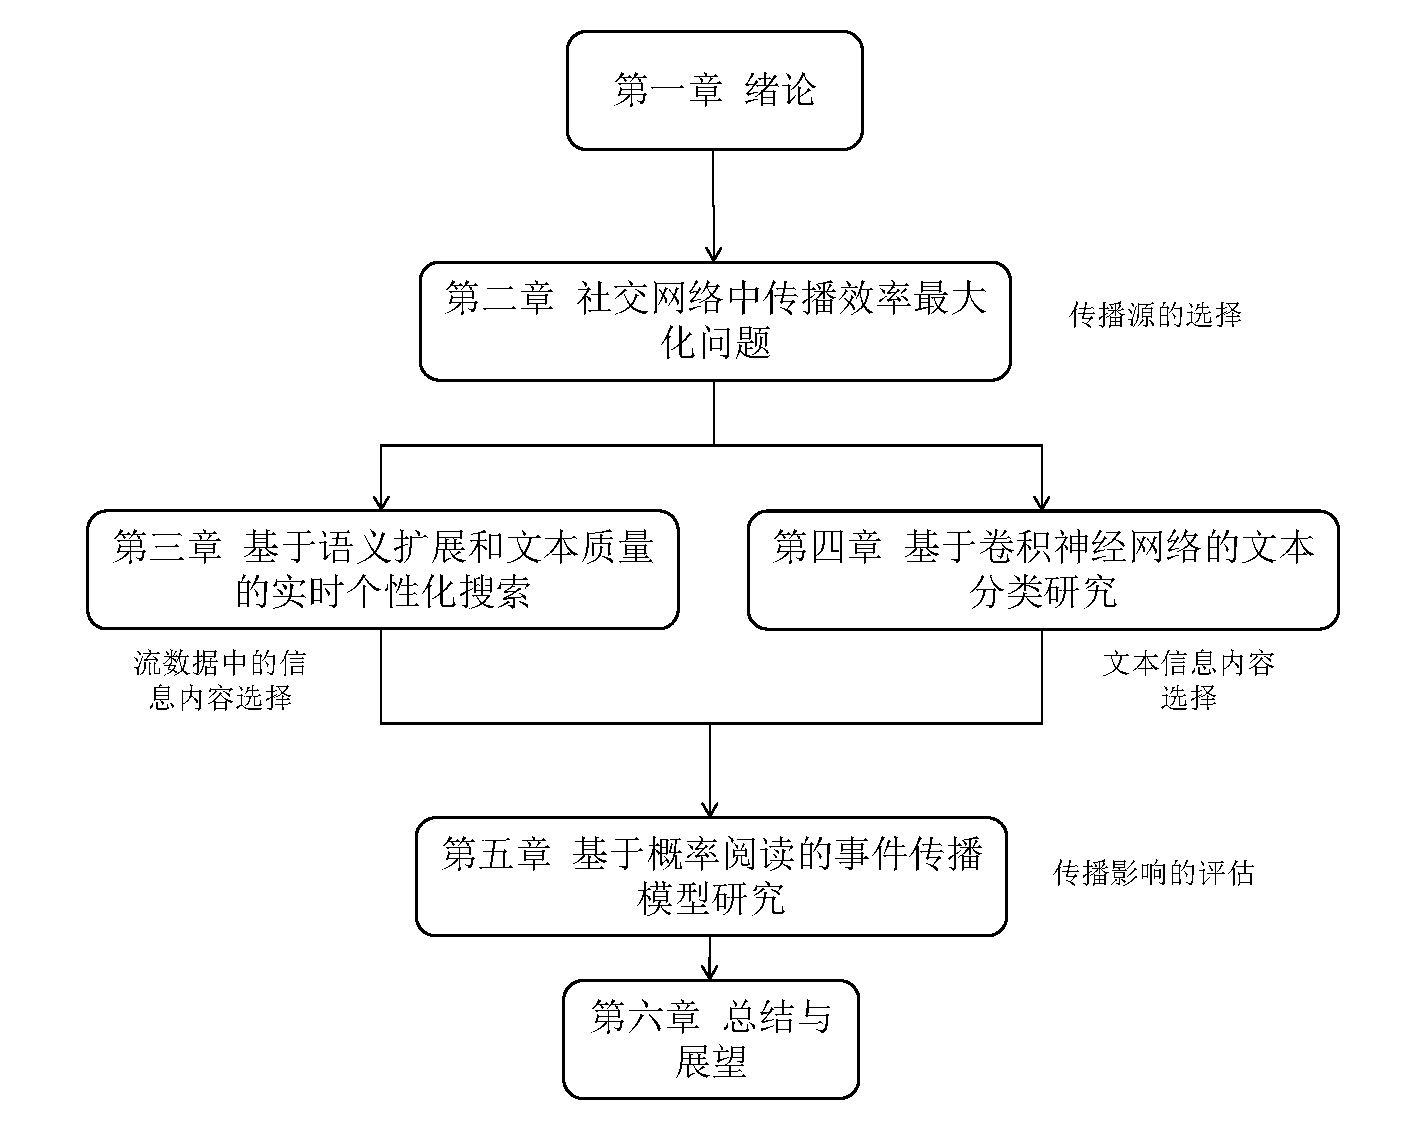
\includegraphics[width=0.8\textwidth]{paperStructure}
    \caption{论文组织结构图}
    \label{fig:paperStructure}
\end{figure}

第一章为绪论,阐述了本文的研究背景与与研究意义,同时对已有的相关研究工作进行了详细的总结,并且概括了本文的研究内容以及创新点。

第二、三、四、五章分别对社交网络信息传播的不同问题进行了研究。第二章研究在社交网络中如何选择传播源的问题,基于传统的影响力最大化问题,考虑传播时延,提出了传播效率最大化问题。第三、四章分别在不同的场景下研究如何选择传播内容的问题。第三章面向社交网络中的流数据,结合语义扩展以及质量模型提出了实时个性化搜索的框架。第四章面向社交网络中的文本数据,应用深度学习技术,提出了一种基于卷积神经网络的文本分类算法。第五章研究社交网络中信息传播的量化问题,以事件为粒度,结合多源信息网络融合、垃圾用户去重以及概率阅读模型,提出了一种新的传播模型用于衡量事件的传播范围。

第六章对本文的工作进行了总结,并对本领域的下一步研究进行了展望。
\chapter{基于语义扩展和文本质量的实时个性化搜索}
\label{2chap:main}
随着社交网络中信息爆炸式的增长,用户越来越难以从海量的信息中获取到自身所需的信息,用户所需的信息往往淹没在其中,这种现象可称之为\textbf{信息洪流}(\textit{information flood})现象。在社交网络、电子商务网站、即时通信等应用中,信息产生的速率以及数量都是过去无法比拟的,如在推特(Twitter)、脸书(Facebook)、新浪微博等社交媒体中,每天都会产生海量的文本信息。根据用户输入的查询,在海量的信息流中实时地检索出高质量的、相关的信息是一个极具挑战性的问题。社交网络中的信息流实时个性化搜索相对于传统的信息检索提出了以下挑战:(1)社交网络中充斥着各种各样话题的信息,而且信息大多数都是以短文本表示,相对于传统的新闻等长文本信息,难以进行语义理解;(2)社交网络中的信息质量参差不齐,难以从中遴选出高质量的信息;(3)社交网络中的信息产生速率快,如何能够实时地检索出用户所需要的信息,将其推送给用户也是一大难点。因此,由于社交网络中数据的信息海量性、主题多样性、数据稀疏性以及社交互动性等特性,传统的个性化检索方法不足以解决社交网络中的信息实时个性化搜索问题。本章针对以上的问题,提出了一个面向推特信息流的实时个性化搜索框架来实现用户的信息实时推荐。本章针对社交网络中信息的特性,提出了一种基于语义扩展和文本质量的实时个性化搜索算法,并在TREC 2015 Microblog Track\upcite{lin2015overview} 测评中验证了算法的性能。首先,我们构造了一个逻辑规则过滤器来选择核心关键词,提高检索的准确率。其次,我们对文本质量进行建模,利用的标注的数据进行训练,以此来对文本的质量的进行打分。训练好的文本质量模型提高了检索的排序性能。然后,我们使用外部语料库来实现语义扩展,例如搜索引擎,知识库等。语义扩展能够使得我们更好地理解用户的偏好和兴趣。最后,我们采用了一个动态的推送策略来自动地推送高质量且相关的信息给特定的用户,这能够避免信息过载。本章中的算法结合了社交网络文本的语义特征和社交属性,针对不同的用户搜索,做了综合性地排序。我们使用TREC 2015 Microblog Track中的真实数据流进行了实验,实验结果显示了本章提出的算法在不同测评指标下,与其他算法相比的优越性。

本章的内容组织如下:第\ref{2sec:motivation} 节介绍了研究动机,讨论了在社交网络环境下进行实时个性化搜索的必要性。第\ref{2sec:definition}节介绍了相关定义,对本章中涉及的相关概念和知识进行了符号化的定义。第\ref{2sec:method} 节介绍了方法描述,详细地阐述了本章提出的系统框架和算法。第\ref{2sec:experiment}节进行了实验分析,验证了本章提出的方法,并且分析了实验结果。最后,第\ref{2sec:conclusion}对本章的内容进行了总结。

\section{研究动机}
\label{2sec:motivation}
随着大数据时代的到来,诸如推特(Twitter)、脸书(Facebook)、新浪微博等的社交网络平台逐渐取代传统的媒体平台,成为新时代的实时信息交互平台。以推特平外为例,据统计,每天平均约有58,000,000条推文(tweet)发布,每天平均处理约2,100,000,000次搜索查询,每月约有115,000,000个活跃的用户\footnote{\url{http://www.statisticbrain.com/twitter-statistics/}}。 在大数据时代,人人都可以是信息的生产者、传播者和接收者,这在一定程度上加速了信息的传播速率。然而,如此庞大的数据量使得用户在社交网络平台中搜索查询时面临了信息过载的问题,用户很难检索到自己需要的信息,亦或用户所需的信息淹没在了众多的信息之中。尤其是社交网络平台中的信息内容囊括了众多领域,其中的话题种类繁多,这使得用户难以搜索到相关性强而且高质量的文本信息。在社交网络平台中,传统的信息检索方法变得耗时长而且信息检索方式难以适用。因此,在大数据时代,为了满足用户实时获取相关信息的需求,需要一种面向社交网络的新的信息检索方法。

在传统的信息检索流程中,往往是用户根据自己所需,输入关键字进行查询,系统根据用户的查询,搜索到相关的结果,并进行排序,返回给用户。而在社交网络平台中,信息产生速率快,信息以数据流的形式给出,同时用户希望系统能够自动地推送相关的信息,而不是用户通过查询来获取信息。因此,在社交网络中的信息实时个性化搜索的流程与传统的信息检索流程不尽相同。在社交网络中,信息的实时个性化搜索流程一般是用户将查询搜索以关键词的形式给出,然后系统根据用户的查询在信息流中实时地处理文本信息,将相关的信息自动地推送给用户。

由美国国家标准与技术研究院(NIST)主办的文本检索会议(TREC)是由多个测评项目组成的一个致力于解决新时代信息检索问题的测评大会,涉及智能问答、医疗诊断、实体识别、信息推荐等领域。TREC自2011年起设立了微博实时推荐(Microblog Track)\upcite{ounis2011overview,soboroff2012overview,lin2013overview,lin2014overview,lin2015overview} 这一个子任务,目标是解决在社交网络中信息的实时个性化搜索问题。从设立后,TREC Microblog Track便吸引了全世界的参赛者参加,与智能实时问答(TREC LiveQA Track)成为了TREC中最火热的两个子任务。Microblog Track 的任务是针对不同用户,智能地分析用户的兴趣爱好,自动地、实时地为用户推送相关的、高质量的信息,涉及到众多科学领域,包括机器学习、自然语言处理、信息检索、人工智能等。如图\ref{fig:twitter_search}所示,在社交网络平台中,用户是信息的生产者,用户将源源不断地发布信息,其中包括有趣的信息和一些无用的信息。同时,用户又是信息的接收者,用户通过定制自身感兴趣的话题和内容,系统智能地分析其兴趣爱好,针对不同的用户,在推特信息流中自动地、实时地为用户推荐相关的、高质量的信息。例如将饮食信息推荐给美食家、将财经信息推送给金融家、将商旅信息推送给旅行者等,同时将一些低质量无意义或者无人关注的信息丢弃。

\begin{figure}[!htbp] % use float package if you want it here
  \centering
  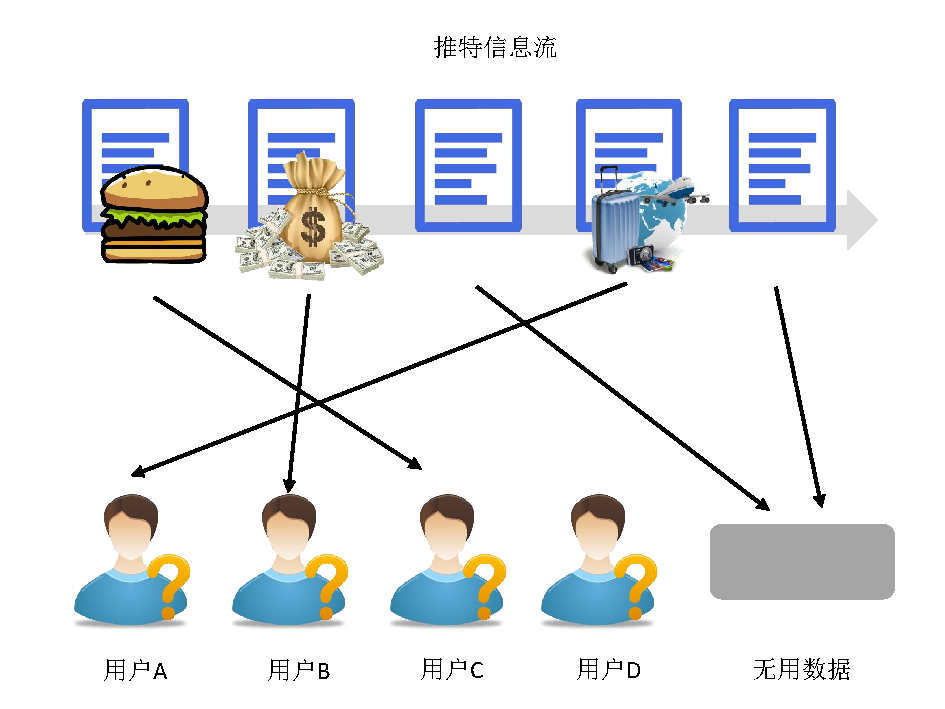
\includegraphics[width=0.8\textwidth]{twitter_search}
  \caption{社交网络平台中信息的实时个性化搜索示意图}
  \label{fig:twitter_search}
\end{figure}

为了解决针对不同用户,为其实时地搜索出相关性强、高质量的信息,许多已有的个性化推荐\upcite{Xie2015Personalized,sontag2012probabilistic,wang2013personalized,tang2015personalized} 以及协同搜索\upcite{liang2014Collaborative,vosecky2014collaborative,xue2009user,yang2014survey} 的工作对这个问题进行了一定的研究。但是很少有面向社交网络个性化搜索的研究,特别是对于实时搜索推荐技术的研究。目前已有的机器学习、自然语言处理、信息检索、人工智能等研究对于社交网络中的实时个性化搜索问题提供了许多帮助。文本分类以及排序的研究\upcite{canuto2015efficient,severyn2015learning,ren2014hierarchical,paik2013novel} 能够为了社交网络中的信息检索提供支持。同时,查询分析以及优化技术\upcite{gao2013query,Letelier2012Static,si2014users} 能够使得信息检索有着显著的提升。

然而,社交网络的环境与传统的新闻、论坛等Web环境有着较大的区别。因此,为了满足社交网络中用户获取信息的需求,这将需要建立新的模型、研究新的方法来解决这一问题。在社交网络中,实现信息的个性化实时推荐面临的主要挑战可以总结如下:
\begin{itemize}
  \item \textbf{信息海量性},在社交网络中,信息产生的速率快,网络中的每一个用户同时扮演着信息生产者、信息传播者和信息接收者的角色。如此高容量的信息流需要一个新的模型来适应持续不断变化的语义特征。
  \item \textbf{主题多样性},社交网络中的信息内容包罗万象,覆盖了许许多多的领域和话题。如果主题模型不能区分众多的话题,这将导致噪声的引入以及不准确的话题模型以及用户模型。
  \item \textbf{数据稀疏性},在社交网络中,信息在不同的主题上的分布是不均匀的,在某些主题上信息量大,而在某些主题上信息是稀疏的。有效的主题模型需要解决数据稀疏性所带来了的影响。
  \item \textbf{社交互动性},社交网络中的用户之间有着丰富的互动信息,与传统的文本信息不同,社交网络中的信息包含了许多有价值的结构化的社交属性。适当地利用这些社交属性能够提高搜索的性能,但是这需要对这些社交属性进行相关性的选择。
\end{itemize}

为了解决上述面临的挑战,本章提出了一种基于语义扩展和文本质量的实时个性化搜索框架,该框架综合考虑了用户的偏好、语义特征和社交属性。首先,本章基于语义扩展提出了一种布尔逻辑关键词过滤(Boolean Logic Keyword Filter)的用户模型。该模型依靠外部搜索引擎提供的知识进行建立,建立的用户模型充分利用了查询扩展以及检索结果的重排序来提高推荐结果的相关性。最终的实验评估证明该模型显著地提高了检索的召回率。此外,本章还基于逻辑回归提出了一种文本质量模型,该模型利用推文的社交属性来评估其文本的质量。该模型能够对推文的文本内容,是否受到大众的认可等进行评估,因此它能帮助系统返回高质量的推文。最终的实验评估证明该模型显著地提高了检索结果的排序性能。

\section{相关定义}
\label{2sec:definition}
本节首先将对社交网络中的实时个性化搜索的任务进行定义,并将其形式化,然后对TREC 2015 Microblog Track的具体任务进行描述。

社交网络中的实时个性化搜索任务可以描述如下。在社交网络中平台中,令信息流表示为\textbf{T},信息流在社交网络中随着时间不断地产生,信息流\textbf{T}中包含许多种类的话题。令\textbf{P}表示用户集合,每一个用户$p_i \in \textbf{P}$表示着用户感兴趣的一个话题,用户的兴趣爱好可以通过文本等形式来表示。则社交网络中的实时个性化搜索任务可以定义如下,
\begin{mydef}[实时个性化搜索]\label{def:realPrnzdSearch}
在社交网络中,给定信息流\textbf{T}以及用户集合\textbf{P},实时个性化搜索的目的是针对不同的用户兴趣爱好$p_i \in \textbf{P}$,自动地实时地为其推荐高质量的、相关的信息。
\end{mydef}

根据定义\ref{def:realPrnzdSearch}可知,社交网络中的实时个性化搜索需要解决的几个核心关键问题如下。首先是如何表示信息流与用户,其次是如何实现实时推荐,以及如何保证信息的高质量和高相关性。社交网络平台中信息的实时个性化搜索任务可以通过图\ref{fig:real-timeSearch}来表示。
\begin{figure}[!htbp] % use float package if you want it here
  \centering
  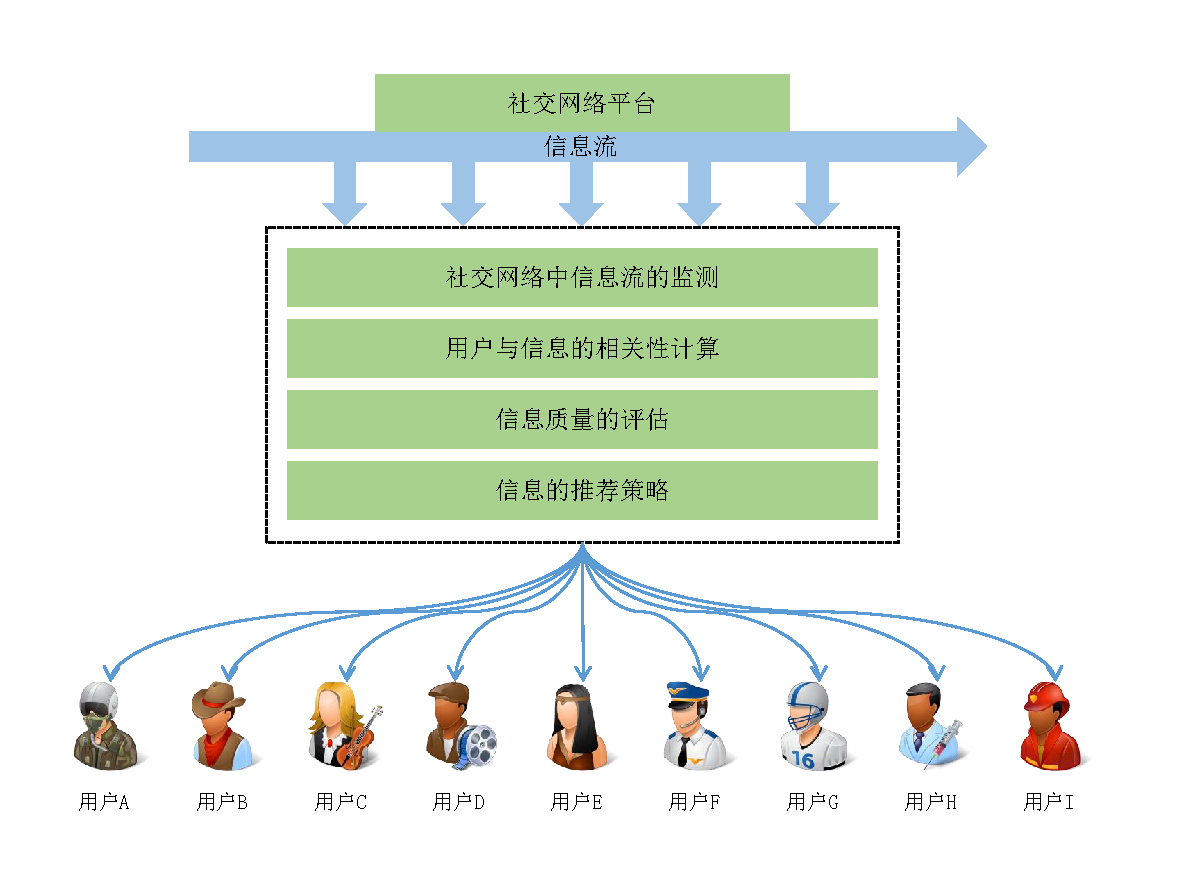
\includegraphics[width=\textwidth]{real-timeSearch}
  \caption{社交网络平台中信息的实时个性化搜索任务图}
  \label{fig:real-timeSearch}
\end{figure}

任务首先要求系统能够实时地监测社交网络中的信息流,然后对不同的用户建立兴趣模型,分析信息与用户之间的相关性。同时任务还要求系统能够对信息的质量做出评估,包括真实性、内容丰富性等。最后,系统需要采取一个良好的推送策略,使得用户不至于淹没在信息中。

TREC 2015 Microblog Track的任务目标是\textbf{实时信息流过滤},实质上也是实时个性化搜索的一种形式。在Microblog Track中,实时信息流过滤的任务目标是根据不同用户的兴趣模型来监测社交媒体中的信息流。值得注意的是,上述的兴趣模型的概念是不同于传统的临时查询。该场景中,交互流程不是用户输入一次查询,然后系统返回结果给用户。该场景不存在实际的查询,取而代之的是系统根据用户的兴趣模型主动地推送\textbf{有趣的}信息给用户。

什么样的信息是有趣的可以考虑如下两个实际的任务模型来帮助更好地理解。
\begin{itemize}
  \item \textbf{场景A:即时性信息推送},在场景A中,用户是定位在使用移动设备的场景,用户可以即时地查看消息。系统基于用户的兴趣模型来判别消息之于用户是否是有趣的,被系统判别为有趣的信息将实时地推送到用户的移动设备(例如手机、平板等)。场景A中的任务目的是上述的推送需要在消息产生的相对较短的时间内完成,该场景中的信息假设是相对较短的。
  \item \textbf{场景B:周期性邮件摘要},在场景B中,用户是定位在使用固定设备的场景,用户周期性的查看消息。与场景A相同,统基于用户的兴趣模型来判别消息之于用户是否是有趣的。但是被系统判别为有趣的信息将被聚集成一个邮件摘要,并且周期性的推送给用户。该场景中的每一个单一信息假设是相对较短的,聚集成的邮件摘要可能很长,我们可以认为这是\textbf{个性化头条新闻}。
\end{itemize}

两个场景都假设推送给用户的消息相对较短,是短消息。因此,推送的消息是否有趣可以根据用户阅读消息的长度或者条数来进行衡量。可以看出,TREC 2015 Microblog Track的任务目标是在两种不同的场景中来考虑社交网络平台中信息的实时个性化搜索问题。

任务中的推特信息流一条推文以JSON格式保存,字段信息如表\ref{2tab:tweetJSON}所示。
\begin{table}[!htbp]
\centering
\caption{推文JSON数据的部分字段信息}
\begin{tabular}{|p{4cm}|p{7cm}|}
\hline
\textbf{字段} & \textbf{描述} \\
\hline
$created\_at$ & 推文的创建时间\\
\hline
$id$ & 推文的ID\\
\hline
$text$ & 推文的文本信息\\
\hline
$source$ & 推文的发布终端\\
\hline
$in\_reply\_to\_status\_id$ & 回复的推文的ID\\
\hline
$user$ & 发布推文的用户信息\\
\hline
\end{tabular}
\label{2tab:tweetJSON}
\end{table}

表\ref{2tab:tweetJSON}中$created\_at$是推文创建的时间,即发布时间。$id$是推文的ID,是唯一的。$text$是推文的文本信息,为短文本,不超过140个字符,可能存在超链接。$source$是推文的发布平台,例如推特Web端,推特手机端,或者通过其他的平台转发至推特等。$in\_reply\_to\_status\_id$是指该推文是否为转发回复其他的推文,如果不是则字段为$null$,如果是则为转发的推文的ID。$user$是指发布推文的用户,也是一个JSON格式的数据,其字段内容在表\ref{2tab:userJSON}中给出。
\begin{table}[!htbp]
\centering
\caption{用户JSON数据的部分字段信息}
\begin{tabular}{|p{4cm}|p{7cm}|}
\hline
\textbf{字段} & \textbf{描述} \\
\hline
$created\_at$ & 用户的创建时间\\
\hline
$id$ & 用户的ID\\
\hline
$screen\_name$ & 用户的名称\\
\hline
$location$ & 用户的地理信息\\
\hline
$description$ & 用户的自我描述\\
\hline
$followers\_count$ & 用户的粉丝数\\
\hline
$friends\_count$ & 用户的好友数\\
\hline
$favourites\_count$ & 用户收藏推文的数目\\
\hline
$statuses\_count$ & 用户发布推文的数目\\
\hline
$utc\_offset$ & 用户所在时区\\
\hline
$profile\_image\_url$ & 用户的头像\\
\hline
$lang$ & 用户的语种\\
\hline
\end{tabular}
\label{2tab:userJSON}
\end{table}

表\ref{2tab:userJSON}中$created\_at$为用户账号建立的时间。$id$为用户的ID,是唯一的。$screen\_name$为用户的名字。$location$为用户的地理位置,由用户自己填写。$description$为用户对自己的描述,为一段文本信息。$followers\_count$为用户的粉丝数,即关注该用户的用户数。$friends\_count$为用户的好友数,即用户关注的用户数目。$favourites\_count$为用户收藏的推文的数目。$statuses\_count$为用户历史上发布推文的数目。$utc\_offset$为用户所在的时区的偏差值,单位为秒。$profile\_image\_url$为用户的头像,如果用户没有自定义头像,则为系统默认头像。$lang$为用户的常用语言。
%在实时信息流过滤任务中,信息即为推文。在测评阶段,进行测评的系统将监测推特的实时样本信息流并根据用户的兴趣模型(相当于特定的话题)来识别有趣的信息。为了描述的简洁性,我们将上述过程称之为\textbf{兴趣用户的追踪}。

\section{方法描述}
\label{2sec:method}
在本节中,我们设计了一个面向社交网络的实时信息流推荐的系统框架。首先,与传统的信息检索系统相似,信息以及用户的语义特征被提取出来,数据的预处理用于过滤掉此阶段中无用的信息。其次,为了计算信息与用户之间的相似度(即相关性),基于外部语料库训练得到的词向量模型来表述提取的特征。除此之外,系统将文本的质量也考虑在内。高质量的文本往往包含高质量的信息,本节提出了一个基于逻辑回归模型的文本质量评估算法来对文本的质量进行衡量。然后,基于得出的相关性与质量,系统针对不同的用户对信息进行评估。一条相关的、有意思的信息将被归类到最相关的类别中,即归类到最相关的用户。最后,为了避免信息洪流、保持消息推送的实时性,本节提出了一个动态的推送策略。因此,用户将实时地收到相关性强、质量高的信息,并且能够避免淹没在信息中。

\subsection{系统框架}
\label{2subsec:systemOverview}
目前在社交网络中,用户只能接收到其关注用户的信息推送,而且这些信息只是简单的按照时间进行排序。理想的搜索系统应当能够分析用户的兴趣爱好,并且自动地推送相关的、高质量的信息给用户。为了满足这一需求,一个面向推特的实时个性化搜索系统的框架设计如图\ref{fig:systemFramework}所示。
\begin{figure}[!htbp] % use float package if you want it here
  \centering
  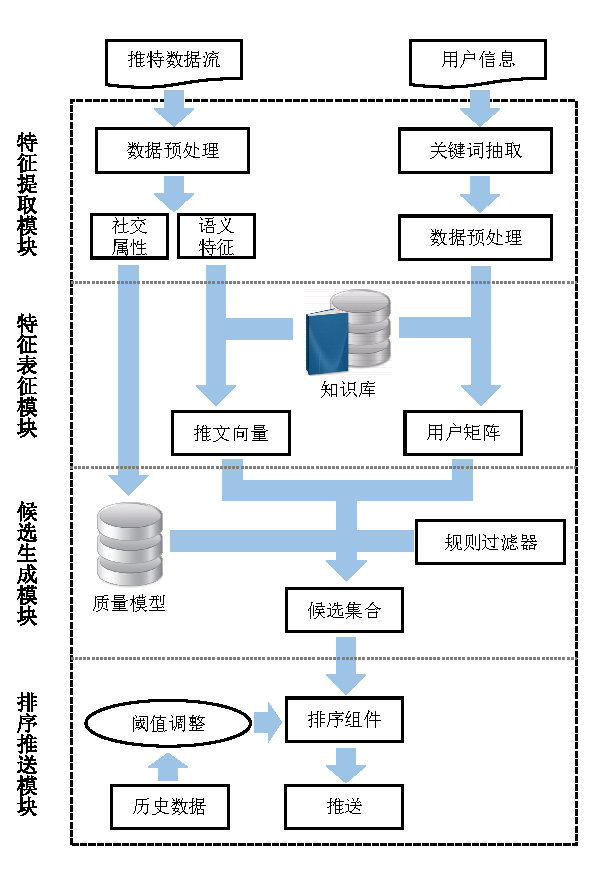
\includegraphics[width=0.7\textwidth]{systemFramework}
  \caption{实时个性化搜索系统框架图}
  \label{fig:systemFramework}
\end{figure}

如图所示,系统主要包括四个主要的模块,分别如下所示。
\begin{itemize}
  \item \textbf{特征提取模块},该模块监测推特信息流,并且接收用户的搜索请求。值得注意的是,在实时个性化搜索任务中,用户的搜索请求相当于某个话题内容的订阅。用户事先输入搜索后,在相关的信息发布时实时推送给用户。推特信息流通过TREC-API\footnote{\url{https://github.com/lintool/twitter-tools}}工具监测。用户的搜索由官方提供,以$p_i \in \textbf{P}$表示。在特征提取之前,数据的预处理将用来过滤掉无用的信息。对于推特信息流,系统提取其语义特征以及社交属性;对于用户信息,系统提取搜索中的关键词作为基础特征。
  \item \textbf{特征表征模块},该模块通过几种技术来扩展及表征所提取的语义特征。推文信息以及用户信息通过该模块进行了语义增强,该模块使得推文以及用户之间的相关度计算更加的方便。
  \item \textbf{候选生成模块},该模块通过语义特征以及社交属性将推文分类到与之最相关的用户。这一过程同时考虑了相关性以及推文的质量,因此用户收到的信息不仅是有趣的而且是高质量的。
  \item \textbf{排序推送模块},该模块通过最终的得分来对每个用户的推文候选队列进行排序,并且利用历史数据进行阈值的动态调整。该模块能够保证用户不错过重要的高质量的信息,又不至于淹没在过多的信息中。
\end{itemize}

在之后的小节中,我们将详细地介绍每一个模块应用的算法以及实现。

\subsection{特征提取模块}
\label{feaureExtraction}
推文信息依靠监测推特的抽样信息流来获取\upcite{wang2015assessor}。在获取到推文后,数据的实时预处理用来过滤掉此阶段内无效的信息,减少无意义的以及冗余的信息。推特数据流上的相关数据预处理方法包含如下一些技术,
\begin{itemize}
  \item \textbf{语言识别},根据任务要求,非英文的推文将被直接过滤掉来简化问题的复杂度。本系统中使用的工具为\textbf{无限元模型语言识别}(\textit{Language Detection with Infinity Gram}),简称为ldig\footnote{\url{https://github.com/shuyo/ldig}}。ldig工具是一个针对短文本消息(例如推特)的语言识别器,能够支持对于17种语言的识别,准确率达到了99.1\%。除此之外,系统还使用了基于字符编码集的语言识别方法来区分英文句子和非英文句子。通过训练得出一个阈值,包含英文字符多的推文将被保留,其余的将被过滤掉。
  \item \textbf{冗余过滤},社交网络中由于复制,转发等行为使得相同信息的推文存在着很多的冗余,如果不进行冗余过滤,那么将会有很多相同的内容推送给用户,使得用户淹没在重复的信息中。因此,对于内容相同或者相似的推文,系统只保存一个副本。为了实现该目标,一种方法是利用表\ref{2tab:tweetJSON}中提到的推文$id$字段和$in\_reply\_to\_status\_id$字段来识别冗余信息。如果推文是原创信息,则我们记录其$id$值;如果推文是转发信息,则可以检查该推文转发推文的$id$是否已经存在来判别是否是冗余信息。每当一条新的推文被爬取时,首先来检查推文的$id$来做冗余消除。该方法简单有效,能够迅速滤除掉大部分的冗余信息。但是当推文是复制其他推文的信息或者做出微小的改动,则该方法无法识别。因此,另外一种冗余消除技术,$simhash$技术被应用。$simhash$技术是用于处理网页冗余的技术,该方法将一个文档转换成一个数字指纹(即一串定长的0-1编码),被称为\textbf{哈希相似码}。两个文档的哈希相似码之间的汉明距离(\textit{hamming distance})越短,则说明两个文档之间的相似度越大。哈希相似码的计算公式如下所示,
  \begin{equation}
  \label{simhash}
    {\mathbf{s}_{hash}} = sign(\sum\nolimits_{i = 1}^n {{w_i} \cdot {\mathbf{c}_i}} )
  \end{equation}
其中$\mathbf{c}_i$是第$i$个词的哈希码,为一个定长的向量,$w_i$是该词的权重,为标量,$sign$是是一个符号函数,让结果向量中的每一个比特的正数位变成1,负数位变成0。simhash算法的过程大概如下。首先,对文档进行关键词抽取,得到特征$\mathbf{c}_i$和权重$w_i$。然后,对所有特征进行加权的位计算。最后,对得到的结果进行哈希码的生成,这个产生值和具体采用的算法有关,这里采用的一个简单的符号函数。将推文转换成哈希相似码后,我们就可以利用推文之间的汉明距离来判别推文间的相似性,来进行冗余消除。基于推文的$id$进行冗余消除是一种高效的方法,能够解决大多数情况下的问题,但是对于复制或者修改的内容无法识别。simhash算法是基于推文的内容进行冗余消除,能够有效地解决内容相似的推文冗余,但是相比于基于推文$id$的方法耗时会长一些,因为计算哈希相似码的过程将会有额外的计算量。在本章提出的系统中,两种算法被结合起来完成冗余消除。首先利用基于推文$id$的方法进行粗的冗余消除,如果无法判别则计算推文的哈希相似码后,根据汉明距离进行判别。
\end{itemize}

在数据的预处理后,我们将推文信息和用户信息的语义特征和社交属性抽取出来。对于推文,名词以及动词是句子中最重要的部分。因此,退文中的名词以及动词(除去停用词)被抽取出来作为语义特征,并且每一个词都根据其在句子中的重要性得到一个不同的权重。一条推文的语义特征可以表示成$\mathbf{ts} = \{ {w_1}{t_1},{w_2}{t_2},\cdots,{w_n}{t_n}\}$,其中$\mathbf{ts}$表示一条推文,$t_i$表示一个词语,$w_i$为该词语的权重。词语的权重与该词语在句子中的位置、出现的频率等有关。



\section{实验分析}
\label{2sec:experiment}

\section{本章小结}
\label{2sec:conclusion}





%%% Local Variables:
%%% mode: latex
%%% TeX-master: "../main"
%%% End:

\begin{ack}
  衷心感谢导师 xxx 教授和 xxx 副教授对本人的精心指导。他们的言传身教将使我终生受益。

  感谢 \nudtpaper{},它的存在让我的论文写作轻松自在了许多,让我的论文格式规整漂亮了许多。

\end{ack}


%</thesis>
%    \end{macrocode}
%
% 在\LaTeX{}下管理参考文献将极其方便,建议使用Jabref生成条目,
% 用\verb|\cite|(其中\verb|upcite|是上标索引)索引即可。
% \verb|refs.bib|是你的参考文献名。
%    \begin{macrocode}
%<*thesis>
\cleardoublepage
\phantomsection
\addcontentsline{toc}{chapter}{参考文献}
\bibliographystyle{bstutf8}
\bibliography{ref/refs}

\begin{resume}

  \section*{发表的学术论文} % 发表的和录用的合在一起

  \begin{enumerate}[{[}1{]}]
  \addtolength{\itemsep}{-.36\baselineskip}%缩小条目之间的间距,下面类似
  \item Yang Y, Ren T L, Zhang L T, et al. Miniature microphone with silicon-
    based ferroelectric thin films. Integrated Ferroelectrics, 2003,
    52:229-235. (SCI 收录, 检索号:758FZ.)
  \item 杨轶, 张宁欣, 任天令, 等. 硅基铁电微声学器件中薄膜残余应力的研究. 中国机
    械工程, 2005, 16(14):1289-1291. (EI 收录, 检索号:0534931 2907.)
  \item 杨轶, 张宁欣, 任天令, 等. 集成铁电器件中的关键工艺研究. 仪器仪表学报,
    2003, 24(S4):192-193. (EI 源刊.)
  \item Yang Y, Ren T L, Zhu Y P, et al. PMUTs for handwriting recognition. In
    press. (已被 Integrated Ferroelectrics 录用. SCI 源刊.)
  \item Wu X M, Yang Y, Cai J, et al. Measurements of ferroelectric MEMS
    microphones. Integrated Ferroelectrics, 2005, 69:417-429. (SCI 收录, 检索号
    :896KM.)
  \item 贾泽, 杨轶, 陈兢, 等. 用于压电和电容微麦克风的体硅腐蚀相关研究. 压电与声
    光, 2006, 28(1):117-119. (EI 收录, 检索号:06129773469.)
  \item 伍晓明, 杨轶, 张宁欣, 等. 基于MEMS技术的集成铁电硅微麦克风. 中国集成电路, 
    2003, 53:59-61.
  \end{enumerate}

  \section*{研究成果} % 有就写,没有就删除
  \begin{enumerate}[{[}1{]}]
  \addtolength{\itemsep}{-.36\baselineskip}%
  \item 任天令, 杨轶, 朱一平, 等. 硅基铁电微声学传感器畴极化区域控制和电极连接的
    方法: 中国, CN1602118A. (中国专利公开号.)
  \item Ren T L, Yang Y, Zhu Y P, et al. Piezoelectric micro acoustic sensor
    based on ferroelectric materials: USA, No.11/215, 102. (美国发明专利申请号.)
  \end{enumerate}
\end{resume}

%</thesis>
%    \end{macrocode}
%
%<thesis>% 最后,需要的话还要生成附录,全文随之结束。
%    \begin{macrocode}
%<*thesis>
\appendix
\backmatter
% TeX
\chapter{模板提供的希腊字母命令列表}

大写希腊字母:
\begin{table}[htbp]
\centering
\begin{tabular}{llll}
\toprule
$\Gamma$~\verb|\Gamma| & $\Lambda$~\verb|\Lambda| & $\Sigma$~\verb|\Sigma| & $\Psi$~\verb|\Psi| \\
$\Delta$~\verb|\Delta| & $\Xi$~\verb|\Xi| & $\Upsilon$~\verb|\Upsilon| & $\Omega$~\verb|\Omega| \\
$\Theta$~\verb|\Theta| & $\Pi$~\verb|\Pi| & $\Phi$~\verb|\Phi| & \\
\midrule
$\varGamma$~\verb|\varGamma| & $\varLambda$~\verb|\varLambda| & $\varSigma$~\verb|\varSigma| & $\varPsi$~\verb|\varPsi| \\
$\varDelta$~\verb|\varDelta| & $\varXi$~\verb|\varXi| & $\varUpsilon$~\verb|\varUpsilon| & $\varOmega$~\verb|\varOmega| \\
$\varTheta$~\verb|\varTheta| & $\varPi$~\verb|\varPi| & $\varPhi$~\verb|\varPhi| & \\
\bottomrule
\end{tabular}
\end{table}

小写希腊字母:
\begin{table}[htbp]
\centering
\begin{tabular}{llll}
\toprule
$\alpha$~\verb|\alpha| & $\theta$~\verb|\theta| & $o$~\verb|o| & $\tau$~\verb|\tau| \\ 
$\beta$~\verb|\beta| & $\vartheta$~\verb|\vartheta| & $\pi$~\verb|\pi| & $\upsilon$~\verb|\upsilon| \\ 
$\gamma$~\verb|\gamma| & $\iota$~\verb|\iota| & $\varpi$~\verb|\varpi| & $\phi$~\verb|\phi| \\ 
$\delta$~\verb|\delta| & $\kappa$~\verb|\kappa| & $\rho$~\verb|\rho| & $\varphi$~\verb|\varphi| \\ 
$\epsilon$~\verb|\epsilon| & $\lambda$~\verb|\lambda| & $\varrho$~\verb|\varrho| & $\chi$~\verb|\chi| \\ 
$\varepsilon$~\verb|\varepsilon| & $\mu$~\verb|\mu| & $\sigma$~\verb|\sigma| & $\psi$~\verb|\psi| \\ 
$\zeta$~\verb|\zeta| & $\nu$~\verb|\nu| & $\varsigma$~\verb|\varsigma| & $\omega$~\verb|\omega| \\ 
$\eta$~\verb|\eta| & $\xi$~\verb|\xi| & $\varkappa$~\verb|\varkappa| & $\digamma$~\verb|\digamma| \\ 
\midrule
$\upalpha$~\verb|\upalpha| & $\uptheta$~\verb|\uptheta| & $\mathrm{o}$~\verb|\mathrm{o}| & $\uptau$~\verb|\uptau| \\ 
$\upbeta$~\verb|\upbeta| & $\upvartheta$~\verb|\upvartheta| & $\uppi$~\verb|\uppi| & $\upupsilon$~\verb|\upupsilon| \\ 
$\upgamma$~\verb|\upgamma| & $\upiota$~\verb|\upiota| & $\upvarpi$~\verb|\upvarpi| & $\upphi$~\verb|\upphi| \\ 
$\updelta$~\verb|\updelta| & $\upkappa$~\verb|\upkappa| & $\uprho$~\verb|\uprho| & $\upvarphi$~\verb|\upvarphi| \\ 
$\upepsilon$~\verb|\upepsilon| & $\uplambda$~\verb|\uplambda| & $\upvarrho$~\verb|\upvarrho| & $\upchi$~\verb|\upchi| \\ 
$\upvarepsilon$~\verb|\upvarepsilon| & $\upmu$~\verb|\upmu| & $\upsigma$~\verb|\upsigma| & $\uppsi$~\verb|\uppsi| \\ 
$\upzeta$~\verb|\upzeta| & $\upnu$~\verb|\upnu| & $\upvarsigma$~\verb|\upvarsigma| & $\upomega$~\verb|\upomega| \\ 
$\upeta$~\verb|\upeta| & $\upxi$~\verb|\upxi| & & \\ 
\bottomrule
\end{tabular}
\end{table}

希腊字母属于数学符号类别,请用\verb|\bm|命令加粗,其余向量、矩阵可用\verb|\mathbf|。


\end{document}
%</thesis>
%    \end{macrocode}
%
% 当然还有一些收尾工作,校验审阅自不必说。接下来你需要:修改论文中英文日期,
% 生成盲评,生成明(盲)评A3封面。
%
% {\color{blue}Happy \TeX{}ing! 欢迎提各式各样的意见!}
%
% \newpage\relax%
%
% \StopEventually{\PrintChanges}
% \clearpage
%
% \section{实现细节}
% 我们首先介绍文档模板的基本信息以及宏包和配置,
% 然后依照国防科学技术大学论文模板的书写规范一节一节的介绍实现步骤。
%
% \changes{v1.2}{2009/09/28}{添加了A3封面制作}
%
% \subsection{基本信息}
%    \begin{macrocode}
%<cls>\NeedsTeXFormat{LaTeX2e}[1999/12/01]
%<cls>\ProvidesClass{nudtpaper}
%<cfg>\ProvidesFile{nudtpaper.cfg}
%<cls|cfg>[2011/07/17 v2.2 NUDT paper template]
%    \end{macrocode}
%
% \subsection{宏包配置}
%
%<*cls>
%
%\changes{v0.99}{2009/08/17}{add package options}
% 当前的宏包选项在之前已经介绍了,下面是实现步骤,就是几个\verb|if|。
%\changes{v1.6}{2009/12/01}{添加单独的单双面控制}
%\changes{v2.0}{2010/11/09}{添加盲评控制}
%
%    \begin{macrocode}
\newif\ifismaster\ismastertrue
\DeclareOption{master}{\ismastertrue}
\DeclareOption{doctor}{\ismasterfalse}
\newif\ifisanon\isanonfalse
\DeclareOption{anon}{\isanontrue}
\newif\ifistwoside\istwosidefalse
\DeclareOption{twoside}{\istwosidetrue}
\DeclareOption*{\PackageWarning{nudtpaper}{Unknown Option '\CurrentOption'}}
% handle fonts
\newif\ifisttf\isttffalse
\newif\ifisotf\isotffalse
\newif\ifisfz\isfzfalse
\newif\ifisfandol\isfandolfalse
\DeclareOption{ttf}{\isttftrue}
\DeclareOption{otf}{\isotftrue}
\DeclareOption{fz}{\isfztrue}
\DeclareOption{fandol}{\isfandoltrue}
\ProcessOptions\relax
%    \end{macrocode}
%
% 首先调用在文档类书写中需要的过程控制语句,在计算一些\verb|length|时要用到
%    \begin{macrocode}
\RequirePackage{ifthen,calc}
%    \end{macrocode}
%
% 接着我们导入文本类,该模板基于标准的书籍模板book,其默认格式为单面打印。
% 博士论文如需双面打印,必须指定\verb|twoside|选项。双开的含义是章节总是
% 起在右手边,左手空白页为完全的空白页,不包含页眉页脚。
%
% \changes{v1.6}{2009/12/01}{修改开关选项}
%
%    \begin{macrocode}
\ifistwoside
  \LoadClass[a4paper,12pt,openright,twoside]{book}
\else
  \LoadClass[a4paper,12pt,openany]{book}
\fi
%    \end{macrocode}
%
% 我们直接用\textsf{geometry}宏包进行页面边距的设定,调用titlesec设定标题以及页眉页脚,
% 用\textsf{titletoc}设定目录格式。需要改动的可以参考这三个宏包的说明文档。
%
%    \begin{macrocode}
\RequirePackage[includeheadfoot]{geometry}
\RequirePackage[center,pagestyles]{titlesec}
\RequirePackage{titletoc}
%    \end{macrocode}
%
% 文档中另外重要的两个部分是表格和图片。
% 首先来看图片:\textsf{graphicx}宏包是必不可少的,
% 并排图形。\textsf{subfigure} 已经不再推荐,用新的 \textsf{subfig}。
% 加入 \verb|config| 选项
% 以便兼容 \textsf{subfigure} 的命令。浮动图形和表格标题样式。\textsf{caption2} 已经不
% 推荐使用,采用新的 \textsf{caption}。它会自动被 \textsf{subfig} 装载进来。所以可以在
% 后面使用 \textbf{captionsetup} 命令,宏包\textsf{float}的作用是可以用H命令,
% 将浮动对象强制放在这里(副作用是版面可能不好):
%
%    \begin{macrocode}
\RequirePackage{graphicx}
\RequirePackage[config]{subfig}
\RequirePackage{float}
%    \end{macrocode}
%
% 再来看表格:我们采用\textsf{longtable}来处理长的表格,还需要\textsf{array}包;
% 标准的论文需要表格为三线表,这里引用\textsf{booktabs}宏包来处理,
% 这样,我们就可以简单的使用\verb|\toprule|,\verb|\midrule|,\verb|bottomrulle|
% 这样的命令;
% 为了在表格中支持跨行,需要引入\textsf{multirow}包,\textsf{tabularx}的作用是为了使用
% 固定宽度的表格,\textsf{slashbox}可以让我们在表格中使用反斜线:
%    \begin{macrocode}
\RequirePackage{array}
\RequirePackage{longtable}
\RequirePackage{booktabs}
\RequirePackage{multirow}
\RequirePackage{tabularx}
\RequirePackage{slashbox}
%    \end{macrocode}
% 表格和图片的例子可以搜索C\TeX{}论坛或者看示例文件。
%
% 引入\textsf{paralist}来达到比较好看的列表环境
%    \begin{macrocode}
\RequirePackage[neverdecrease]{paralist}
%    \end{macrocode}
%
% 文档中还需要一定的色彩控制和字体控制
%    \begin{macrocode}
\RequirePackage{xcolor}
%    \end{macrocode}
%
% 为了排出漂亮的数学公式,\textsf{amsmath}包是必不可少的,
% 需要注意的是,新版本的论文模不再使用\textsf{txfonts}宏包,
% 为了支持希腊正体字母,需要调用\verb|upgreek.sty|,使用方法是\verb|\up<greek>|。
% 注意到这个宏包前面加上了\verb|Symbolsmallscale|选项,这是为了调整希腊字母的大小而设定的。
% 如果用户不满意这个宏包的积分号
% 等符号,倾向与使用传统的\LaTeX{}风格的数学符号,那么可以使用
% \textsf{mathptmx}宏包,但要把\verb|upgreek|的选项改为\verb|Symbol|,要不然
% 正体希腊字母要显得比正常字符小一点哦。
% 而大写斜体希腊字母(变量)可以通过\textsf{amsmath}的\verb|\var<Greek>|得到。
% 对于希腊字母的加粗使用\verb|bm|宏包,而一般变量的加粗那就使用\verb|\mathbf|吧!
% \changes{v2.0}{2010/11/09}{去掉fontspec,传递no-math到xeCJK,加入bm宏包}
% \changes{v2.2}{2011/07/16}{去掉txfonts宏包,使用lm字体,添加svgreek.sty}
% \changes{v2.2}{2011/07/16}{修改,仍旧使用upgreek, mathptmx, bm组合}
% \changes{v2.2}{2011/09/25}{修改,使用upgreek, txfonts, bm组合}
% \changes{v2.2}{2012/11/28}{给用户提供额外的选项,还是mtpro比较漂亮}
% \changes{v2.3}{2013/12/27}{调整数学字体,加入mtpro使用说明,并且仿照IEEE模板,修改displaypenalty}
% \changes{v2.5}{2015/05/11}{去掉txfonts,用默认数学字体}
%    \begin{macrocode}
\RequirePackage{amsmath,amssymb}
\RequirePackage[Symbolsmallscale]{upgreek}
%\RequirePackage{amsmath}
%\RequirePackage[amsbb,eufrak,compatiblegreek,subscriptcorrection,nofontinfo]{mtpro2}
\interdisplaylinepenalty=2500
\RequirePackage{bm}
\RequirePackage[T1]{fontenc}
\RequirePackage[amsmath,thmmarks,hyperref]{ntheorem}
%    \end{macrocode}
% 需要注意的是,如果用户有\verb|mtpro2|包,还是强烈建议使用这个的,因为数学公式
% 在这个包下显得特别的美观。虽然下载和安装不属于这篇使用说明的范畴,但是,上面的注释部分
% 可以给大家如何使用的一个简单的例子。当你安装好\verb|mtpro2|之后,主要取消注释,并且将
% 上面的三个包注释掉即可。
%
% 本文档类直接采用\XeTeX{}引擎,方便了字体配置以及编译,
% 这里需要调用\textsf{XeCJK}宏包,no--math的作用是不改变先前数学宏包设定的数学字体。
% 同时采用\textsf{indentfirst}宏包管理文字的缩进:
% \changes{v1.8}{2010/10/15}{修改了默认的xeCJK的选项,为了兼容旧的xeCJK版本,normalindentfirst选项暂不使用,而是在后面添加indentfirst包}
% \changes{v2.0}{2010/11/10}{传递no-math给xeCJK里面的fontspec宏包}
% \changes{v2.2}{2011/07/03}{移除CJKtextspace, CJKmathspace, CJKnumber选项}
% \changes{v2.4}{2015/02/09}{移除CJKnumber选项,添加新的CJKnum宏包。旧版本TexLive无需更改。}
%
%    \begin{macrocode}
\RequirePackage[CJKchecksingle,no-math]{xeCJK}
\RequirePackage{CJKnumb}
\RequirePackage{indentfirst}
%    \end{macrocode}
%
% 另外一个关键部分是文献索引,包括书签以及参考文献的索引,记得\textsf{hyperref}配合
% \XeTeX{}使用时暂不能开启Unicode选项,新的发行版已经移除\textsf{hypernat}包。
% 另外还要注意,你最终的打印版肯定不希望有花花绿绿的链接对吧?
% 那就把下面那行\verb|hyperref|注释掉就行了或者把选项改为\verb|\colorlinks=false|即可。
% \changes{v2.1}{2010/12/29}{移除hypernat包}
% \changes{v2.2}{2011/07/17}{移除hyperref的CJKbookmarks旋向}
% \changes{v2.3}{2013/12/27}{加入色彩版hyperref}
% \changes{v2.5}{2015/05/11}{提示用户在最终打印版时去掉链接颜色}
%    \begin{macrocode}
\RequirePackage[numbers,sort&compress,square]{natbib}
\RequirePackage[colorlinks=true,linkcolor=blue,citecolor=red,pdfborder=0 1 1]{hyperref}
%\RequirePackage[pdfborder=0 0 1]{hyperref}
%    \end{macrocode}
%</cls>
%
%\subsection{基础配置}
% 本章主要介绍模板中用到的基本的元素和定义,现在包括两部分: 字体,字号和字体命令
%
%\subsubsection{字体定义}
% 我们首先来处理\TeX{}中最令人棘手的字体问题,
% 在使用\textsf{XeCJK}包之后,配置和选择很容易,
% 预先设定好一些字体命令是为了后面方便的更改文本字体的需要。
% 首先我们开启\TeX{}连字符:
%    \begin{macrocode}
%<*cls>
\defaultfontfeatures{Mapping=tex-text}
%</cls>
%    \end{macrocode}
%
% 之后用\textsc{XeCJK}包提供的命令设定字体,用户可以选择使用TTF还是OTF字体,
% Adobe的OpenType字体在排版上更具备优势,文档显示锐利,推荐使用。
% 另外在这一个新版本中,我们推荐用户也可以使用方正的字体,只要使用\verb|FZ|选项即可。
% 中注释掉相关的字体就可以。方正字体的有点是标点符号的位置无需修正,且字体之间配合很好。
% \verb|setcharclass|的作用是纠正xunicode、xeCJK的一些设定:
%
% \changes{v0.99}{2009/08/17}{add options TTF and OTF}
% \changes{v1.9}{2010/10/28}{定义一个cusong字体,使用的是中宋}
% \changes{v2.3}{2013/12/27}{用户可以考虑使用方正字体,加入FZ选项}
% \changes{v2.5}{2015/05/11}{重新更改字体选项的调用方式,现在变成三个ttf、otf、fz}
% \changes{v2.5}{2015/05/11}{这种方式用户可以特别方便的添加自己的字体集}
%
%    \begin{macrocode}
%<*cls>
\xeCJKsetcharclass{"0}{"2E7F}{0}
\xeCJKsetcharclass{"2E80}{"FFFF}{1}

% ZhongYi 中易字体
\newcommand{\installttf}{
    %%%% Windows Thesis Fonts
    \setmainfont{Times New Roman PS Std}
    \setsansfont{Arial}
    \setmonofont{Courier New}
    %%%% Using Office Family Fonts
    \setCJKmainfont[BoldFont={STZhongsong}]{SimSun}
    \setCJKsansfont{SimHei} % Hei
    \setCJKmonofont{FangSong} % Fangsong 
    %%%% alias
    \setCJKfamilyfont{song}{SimSun}
    \setCJKfamilyfont{hei}{SimHei}
    \setCJKfamilyfont{fs}{FangSong} % fang-song
    \setCJKfamilyfont{kai}{KaiTi} % Kai
}

% Adobe 字体
\newcommand{\installotf}{
    %%%% Windows Thesis Fonts
    \setmainfont{Times New Roman PS Std}
    \setsansfont{Arial}
    \setmonofont{Courier New}
    %%%% Using Adobe Family Fonts
    \setCJKmainfont[BoldFont={STZhongsong}]{Adobe Song Std}
    \setCJKsansfont{Adobe Heiti Std} % Hei
    \setCJKmonofont{Adobe Fangsong Std} % Fangsong 
    %%%% alias
    \setCJKfamilyfont{song}{Adobe Song Std}
    \setCJKfamilyfont{hei}{Adobe Heiti Std}
    \setCJKfamilyfont{fs}{Adobe Fangsong Std} % fang-song
    \setCJKfamilyfont{kai}{Adobe Kaiti Std} % Kai
}

% fz 方正字体 [recommended]
\newcommand{\installfz}{
    %%%% Windows Thesis Fonts
    \setmainfont{Times New Roman PS Std}
    \setsansfont{Arial}
    \setmonofont{Courier New}
    %%%% Using Founder Family Fonts
    \setCJKmainfont[BoldFont={FZYaSong-DB-GBK}]{FZShuSong_GB18030-Z01}
    \setCJKsansfont{FZHei-B01} % Hei
    \setCJKmonofont{FZFangSong-Z02} % fs
    %%%% alias
    \setCJKfamilyfont{song}{FZShuSong_GB18030-Z01}
    \setCJKfamilyfont{hei}{FZHei-B01}
    \setCJKfamilyfont{fs}{FZFangSong-Z02} % fang-song
    \setCJKfamilyfont{kai}{FZKai-Z03} % Kai
}

% fandol [incomplete in 2015]
\newcommand{\installfandol}{
    %%%% Windows Thesis Fonts
    \setmainfont{Times New Roman PS Std}
    \setsansfont{Arial}
    \setmonofont{Courier New}
    %%%% Using Fandol Family Fonts
    \setCJKmainfont{FandolSong}
    \setCJKsansfont{FandolHei} % Hei
    \setCJKmonofont{FandolFang} % fs
    %%%% alias
    \setCJKfamilyfont{song}{FandolSong}
    \setCJKfamilyfont{hei}{FandolHei}
    \setCJKfamilyfont{fs}{FandolFang} % fang-song
    \setCJKfamilyfont{kai}{FandolKai} % Kai
}

\ifisttf
\installttf
\fi

\ifisotf
\installotf
\fi

\ifisfz
\installfz
\fi

\ifisfandol
\installfandol
\fi

%</cls>
%    \end{macrocode}
%
% \changes{v1.6}{2009/12/01}{替换OTF英文字体为标准Windows自带字体}
% \changes{v2.3}{2013/12/27}{添加FZ字体选项}
%
% 选定好字体之后,就是设定字体别名,这样我们就可以在文档的其他部分直接使用较短的命令来
% 指定特定的字体了:
%
%    \begin{macrocode}
%<*cls>
% command alias
\newcommand{\cusong}{\bfseries}
\newcommand{\song}{\CJKfamily{song}}     % 宋体
\newcommand{\fs}{\CJKfamily{fs}}         % 仿宋体
\newcommand{\kai}{\CJKfamily{kai}}       % 楷体
\newcommand{\hei}{\CJKfamily{hei}}       % 黑体
\def\songti{\song}
\def\fangsong{\fs}
\def\kaishu{\kai}
\def\heiti{\hei}
%</cls>
%    \end{macrocode}
%
% \subsubsection{字号定义}
%下面就是定义字号大小,这一部分我们有两个参考,其一是:
%
% \begin{verbatim}
% 参考科学出版社编写的《著译编辑手册》(1994年)
% 七号      5.25pt       1.845mm
% 六号      7.875pt      2.768mm
% 小五      9pt          3.163mm
% 五号      10.5pt       3.69mm
% 小四      12pt         4.2175mm
% 四号      13.75pt      4.83mm
% 三号      15.75pt      5.53mm
% 二号      21pt         7.38mm
% 一号      27.5pt       9.48mm
% 小初      36pt         12.65mm
% 初号      42pt         14.76mm
%
% 这里的 pt 对应的是 1/72.27 inch,也就是 TeX 中的标准 pt
% \end{verbatim}
%
% 另外一个来自WORD中的设定:
% \begin{verbatim}
% 初号 = 42bp = 14.82mm = 42.1575pt
% 小初 = 36bp = 12.70mm = 36.135 pt
% 一号 = 26bp = 9.17mm = 26.0975pt
% 小一 = 24bp = 8.47mm = 24.09pt
% 二号 = 22bp = 7.76mm = 22.0825pt
% 小二 = 18bp = 6.35mm = 18.0675pt
% 三号 = 16bp = 5.64mm = 16.06pt
% 小三 = 15bp = 5.29mm = 15.05625pt
% 四号 = 14bp = 4.94mm = 14.0525pt
% 小四 = 12bp = 4.23mm = 12.045pt
% 五号 = 10.5bp = 3.70mm = 10.59375pt
% 小五 = 9bp = 3.18mm = 9.03375pt
% 六号 = 7.5bp = 2.56mm
% 小六 = 6.5bp = 2.29mm
% 七号 = 5.5bp = 1.94mm
% 八号 = 5bp = 1.76mm
%
% 1bp = 72.27/72 pt
% \end{verbatim}
%
% 我们采用习惯的字号设定方法(也就是WORD中的设定),首先编写字体设置命令:
%
%\begin{macro}{\choosefont}
% 我们可以使用 |\choosefont| 来选择字体, 字体设定这些大多是从清华的模板拷过来的。
%
%    \begin{macrocode}
%<*cls>
\newlength\thu@linespace
\newcommand{\thu@choosefont}[2]{%
    \setlength{\thu@linespace}{#2*\real{#1}}%
    \fontsize{#2}{\thu@linespace}\selectfont}
\def\thu@define@fontsize#1#2{%
    \expandafter\newcommand\csname #1\endcsname[1][\baselinestretch]{%
    \thu@choosefont{##1}{#2}}}
%</cls>
%    \end{macrocode}
%\end{macro}
%
%设定具体的字体大小:
%
%    \begin{macrocode}
%<*cls>
\thu@define@fontsize{chuhao}{42bp}
\thu@define@fontsize{xiaochu}{36bp}
\thu@define@fontsize{yihao}{26bp}
\thu@define@fontsize{xiaoyi}{24bp}
\thu@define@fontsize{erhao}{22bp}
\thu@define@fontsize{xiaoer}{18bp}
\thu@define@fontsize{sanhao}{16bp}
\thu@define@fontsize{xiaosan}{15bp}
\thu@define@fontsize{sihao}{14bp}
\thu@define@fontsize{banxiaosi}{13bp}
\thu@define@fontsize{xiaosi}{12bp}
\thu@define@fontsize{dawu}{11bp}
\thu@define@fontsize{wuhao}{10.5bp}
\thu@define@fontsize{xiaowu}{9bp}
\thu@define@fontsize{liuhao}{7.5bp}
\thu@define@fontsize{xiaoliu}{6.5bp}
\thu@define@fontsize{qihao}{5.5bp}
\thu@define@fontsize{bahao}{5bp}
%</cls>
%    \end{macrocode}
%
%\subsubsection{自定命令}
% 有一些常量,测试,自定义的命令等都放在这里,待到论文逐渐完善之后再做定夺,
% 当然用户自己的命令也可以在此添加,事实上如果natbib传递的是superscript,
% \verb|cite|命令默认就成了上标了。这里不加入这个选项,而是单独编写一个命令:
%
%    \begin{macrocode}
%<*cls>
\newcommand{\upcite}[1]{\textsuperscript{\cite{#1}}} % 上标形式引用
\newcommand{\china}{中华人民共和国}
\def\nudtpaper{\textsc{Nudt}\textsc{Paper}}
\newcommand{\pozhehao}{\kern0.2em\rule[0.8ex]{1.6em}{0.1ex}\kern0.2em}
\newcommand{\xiaopozhe}{\kern0.2em\rule[0.8ex]{0.6em}{0.1ex}\kern0.2em}
%</cls>
%    \end{macrocode}
% \changes{v2.5}{2015/05/11}{添加了一个xiaopozhe命令,用作中文连词符}
%
%\subsubsection{中文元素}
%
% 默认的页面元素的英文名,诸如Contents为目录,Abstract为摘要等,
% 我们首先将他们一一中文化:
% \changes{v0.992}{2009/08/19}{修改图表编号格式}
% \changes{v1.3}{2009/10/14}{修改图目录和表目录}
%
%    \begin{macrocode}
%<*cls>
\renewcommand\contentsname{目\hspace{1em}录}
\renewcommand\listfigurename{图\hspace{1em}目\hspace{1em}录}
\renewcommand\listtablename{表\hspace{1em}目\hspace{1em}录}
\newcommand\listequationname{公式索引}
\newcommand\equationname{公式}
\renewcommand\bibname{参考文献}
\renewcommand\indexname{索引}
\renewcommand\figurename{图}
\renewcommand\tablename{表}
\renewcommand\appendixname{附录}
\def\CJK@today{\CJKdigits{\the\year} 年 \CJKnumber{\the\month} 月}
\newcommand\zhtoday{\CJK@today}
\newcommand\entoday{\today{}}
%</cls>
%    \end{macrocode}
%
% 好,下面就开始按照论文模板要求进行排版!
%
%\subsection{编写要求}
% 学校规定,论文需采用白色纸双面打印。
% 学位论文用A4($210mm\times{}297mm$)标准大小的白纸,
% 在打字或印刷时,要求纸的四周留足空白边缘,以便装订、复制和读者批注。
% 每一面的上方(天头)和下方(地角)分别留边25mm,左侧(订口)
% 和右侧(切口)分别留边30mm,页眉与页脚分别为23mm。
%
% 实现起来很简单,只要调用\textsf{geometry}的版面控制命令即可,
% 方法为先把word模板转化为PDF,
% 用Adobe的裁剪功能查看页边距,进行微调,直到比对正确为止,设定如下:
%
% \changes{v0.991}{2009/08/18}{modify bottom skip}
% \changes{v1.1}{2009/09/26}{修改footskip容限以及bottom的值,为了容下longtab的''下一页''}
% \changes{v1.4}{2009/10/28}{减小页眉skip 1mm,用word叠印}
% \changes{v1.4}{2009/10/30}{增大页眉sep .5mm,用word叠印}
%
%    \begin{macrocode}
%<*cls>
\geometry{top=21mm,bottom=25.5mm,left=30mm,right=30mm}
\geometry{headheight=9mm,headsep=1mm,footskip=9mm}
%</cls>
%    \end{macrocode}
%
%\subsection{页眉页脚}
%
% 我们采用titlesec进行页面配置。
% 页面中的主要元素有Chapter,Section,Subsection等元素的外观,
% 位置,颜色字体等,页面元素还包括页眉页脚。这种方法配置简便,易管理。
% 国防科大的论文需要在页眉处画两根横线,我们通过下面的命令实现:
%
%\begin{macro}{\setheadrule}
% 这个命令属于更改\textsf{titlesec}中的一个画页眉的命令,稍加调整:
% \changes{v0.991}{2009/08/18}{modify headrull, s.t. all geometry match}
% \changes{v1.9}{2010/10/28}{去掉headsep,修改headrule,在sethead后添加raisebox}
%
%    \begin{macrocode}
%<*cls>
\renewcommand\setheadrule[1]{%
  \ifdim#1=\z@
    \let\makeheadrule\@empty
  \else
    \def\makeheadrule{%
    \makebox[0pt][l]{\rule[.2\baselineskip]{\linewidth}{1.5pt}}%
    \rule{\linewidth}{1.5pt}}%
  \fi}
%</cls>
%    \end{macrocode}
%\end{macro}
%
% 由于Chapter第一页默认是\verb|plain|页面格式,
% 章节的其余部分是在Matter中设定的页面格式,为了简单起见,
% 我们就直接更改\verb|plain|页面设置,
% 要求为5号宋体居中放置,画页眉页脚,页脚为1磅黑线
%
% \changes{v0.992}{2009/08/20}{renewpagestyle里面前导的空格可能导致clearpage生成新的一页,将空格去掉}
% \changes{v0.993}{2009/08/26}{修改标题,博士硕士对应不同的页眉}
%
%    \begin{macrocode}
%<*cls>
\renewpagestyle{plain}{
\sethead{}{\raisebox{.65\baselineskip}{\songti \wuhao \ifisanon{~}\else{国防科学技术大学研究生院\@optionpaperclass{}学位论文}\fi}}{}%
\setfoot{}{{\songti \wuhao 第~\thepage~页}}{}%
\headrule%
\footrule%
}
\setfootrule{1bp}
%</cls>
%    \end{macrocode}
%
%\subsection{编写格式}
%
% 当页面设置好之后,就是在论文的不同部分分别调用,一般来说论文类的书籍
% 分为三个matter,为前言区(前置部分),正文区(主体),后文区(附录),
% 在国防科大论文书写要求中,
% 需要将摘要单独进行页码编号,其编号为小写罗马字母,为此,
% 可以将摘要单独设定为一个matter,
% 名叫就叫做MidMatter,称作摘要区。每个Matter我们都一一介绍。
%
% 首先看前置部分,主要包括封面,目录,摘要等,实现为:
%
%    \begin{macrocode}
%<*cls>
\renewcommand\frontmatter{%
    \if@openright\cleardoublepage\else\clearpage\fi
    \@mainmatterfalse
    \pagenumbering{Roman}
    \pagestyle{plain}}
\newcommand\midmatter{%
    \if@openright\cleardoublepage\else\clearpage\fi
    \@mainmatterfalse
    \pagenumbering{roman}
    \pagestyle{plain}}
%</cls>
%    \end{macrocode}
%
% 之后为文章的正文区,采用阿拉伯数字编页码:
%
%    \begin{macrocode}
%<*cls>
\renewcommand\mainmatter{%
    \if@openright\cleardoublepage\else\clearpage\fi
    \@mainmattertrue
    \pagenumbering{arabic}
    \pagestyle{plain}}
%</cls>
%    \end{macrocode}
%
% 最后是附录部分,由于他的章节标题与正文中不一样(不是第几章,而是附录几),
% 我们需要单独设定:
%
%    \begin{macrocode}
%<*cls>
\renewcommand\backmatter{%
    \if@openright\cleardoublepage\else\clearpage\fi
    \titleformat{\chapter}{\filcenter \heiti \sanhao}{附录\,\thechapter\,}{1em}{}
    \titlecontents{chapter}[0pt]{\vspace{0.25\baselineskip} \heiti \xiaosi[1.25]}
      {附录\,\thecontentslabel\quad}{}
      {\hspace{.5em}\titlerule*{.}\contentspage}
    \@mainmattertrue
    \pagestyle{plain}}
%</cls>
%    \end{macrocode}
%
% 我们重新定义\verb|cleardoublepage|,使得生成完全的空白页,页面模式为\verb|empty|
%    \begin{macrocode}
%<*cls>
\renewcommand\cleardoublepage{\clearpage\if@openright \ifodd\c@page\else
  \newpage{}
  \thispagestyle{empty}
  \vspace*{\fill}
  \begin{center}
  \end{center}
  \vspace*{\fill}
  \clearpage\fi\fi%
}
%</cls>
%    \end{macrocode}
%
%\subsubsection{前置目录}
% 前置部分的封面在后面详细介绍。首先看目录,要求为:
% 目次页由论文的章、节、条、项、附录等的序号、名称和页码组成,
% 另页排在序之后。目次页标注学位论文的前三级目录。
% 标题统一用“目录”,黑体3字号字居中,段前、段后间距为1行;
% 各章(一级目录)名称用黑体小4号字,段前间距为0.5行,
% 段后间距为0行; 其它(二、三级目录)用宋体小4号字,
% 段前、段后间距为0行。:
%
% 在\LaTeX{}中,Chapter在目录中默认是没有点的,我们加上,另外我们一并将
% 目录中的section和subsection设定好,
% \changes{v0.991}{2009/08/18}{modify TOC baselineskip and font lineskip to 1.25}
%
%    \begin{macrocode}
%<*cls>
\titlecontents{chapter}[0pt]{\vspace{0.25\baselineskip} \heiti \xiaosi[1.25]}
    {第\CJKnumber{\thecontentslabel}章\quad}{}
    {\hspace{.5em}\titlerule*{.}\contentspage}
\titlecontents{section}[2em]{\songti \xiaosi[1.25]}
    {\thecontentslabel\quad}{}
    {\hspace{.5em}\titlerule*{.}\contentspage}
\titlecontents{subsection}[4em]{\songti \xiaosi[1.25]}
    {\thecontentslabel\quad}{}
    {\hspace{.5em}\titlerule*{.}\contentspage}
%</cls>
%    \end{macrocode}
%
% 然后是表目录和图目录,内容用宋体小4号字,在同学使用模板时,需要标题对齐,
% 我们一并在这里实现:
% \changes{v0.993}{2009/08/25}{添加makebox使得图表标题对齐}
%
%    \begin{macrocode}
%<*cls>
\titlecontents{figure}[0pt]{\songti \xiaosi[1.25]}
    {\makebox[3.5em][l]{图~\thecontentslabel\quad}}{}
    {\hspace{.5em}\titlerule*{.}\contentspage}
\titlecontents{table}[0pt]{\songti \xiaosi[1.25]}
    {\makebox[3.5em][l]{表~\thecontentslabel\quad}}{}
    {\hspace{.5em}\titlerule*{.}\contentspage}
%</cls>
%    \end{macrocode}
%
% 书籍模板中,在LOF或者LOT章节之间会默认插入额外的距离,我们通过修改下面这个命令移除,
% 这个方法不是一个完美的办法,\textbf{注意}:下面的代码不要去深究或者理解,
% 这只是把book.cls中的内容复制过来,然后去掉包含addvspace命令的两行。
% 我实在找不出更加好的办法,如果你有,可以联系我。
%
% \changes{v0.993}{2009/08/25}{移除LOF及LOT中章节之间额外的距离}
%
%    \begin{macrocode}
%<*cls>
\renewcommand\chapter{\if@openright\cleardoublepage\else\clearpage\fi
                    \thispagestyle{plain}%
                    \global\@topnum\z@
                    \@afterindentfalse
                    \secdef\nudt@chapter\@schapter}
\def\nudt@chapter[#1]#2{
  \ifnum \c@secnumdepth >\m@ne
    \if@openright\cleardoublepage\else\clearpage\fi
    \phantomsection
    \if@mainmatter
      \refstepcounter{chapter}%
      \addcontentsline{toc}{chapter}%
        {\protect\numberline{\thechapter}#1}%
    \else
      \addcontentsline{toc}{chapter}{#1}%
    \fi
  \else
    \addcontentsline{toc}{chapter}{#1}%
  \fi
  \chaptermark{#1}%
  \if@twocolumn
    \@topnewpage[\@makechapterhead{#2}]%
  \else
    \@makechapterhead{#2}%
    \@afterheading
  \fi
}
%</cls>
%    \end{macrocode}
%
%\subsubsection{前置摘要}
%
% 摘要的要求为题目黑体3字号字居中,段前、段后间距为1行,内容用宋体小4号字,
% 英文摘要内容用Time New Roman小4号字。
% 中文关键字以黑体小4号字另起一行,排在摘要的下方,英文关键字用Arial小4号字。
%
% \changes{v1.8}{2010/10/15}{ABSTRACT和英文关键字需要用Arial字体}
% \changes{v2.5}{2015/05/11}{英文关键词也要加粗}
%    \begin{macrocode}
%<*cls>
\newcommand\cabstractname{摘\hspace{1em}要}
\newcommand\eabstractname{ABSTRACT}
\newcommand\ckeywordsname{关键词}
\newcommand\ckeywords[1]{{\hei\xiaosi \ckeywordsname: #1}}
\newcommand\ekeywordsname{Key Words}
\newcommand\ekeywords[1]{\textbf{\textsf{\xiaosi \ekeywordsname: #1}}}
\newenvironment{cabstract}{%
    \chapter{\cabstractname}
    \xiaosi
    \@afterheading}
    {\par\vspace{2em}\par}
\newenvironment{eabstract}{%
    \chapter{\textsf{\eabstractname}}
    \xiaosi
    \@afterheading}
    {\par\vspace{2em}\par}
%</cls>
%    \end{macrocode}
%
%\subsection{主体部分}
%
% \subsubsection{标题格式}
% 要求为:
% \begin{compactenum}
% \item	一级标题(章)用黑体3号字居中,1.25倍行距,段前、段后间距为1行,每一章从新的一页开始;
% \item	二级标题(节)用宋体4号粗体字居中,1.25倍行距,段前、段后间距为1行;
% \item	三级标题用黑体小4号字两端对齐,1.25倍行距,段前、段后间距为1行;
% \item	四级标题用宋体小4号粗体字两端对齐,1.25倍行距,段前间距为0.5行,段后间距为0行;
% \end{compactenum}
%
% \changes{v0.991}{2009/08/18}{按照要求设定标题}
% \changes{v0.992}{2009/08/19}{修改secnumdepth使得subsubsection可用}
% \changes{v1.1}{2009/09/26}{修改Title的spacing为弹性值}
% \changes{v1.2}{2009/10/06}{去掉弹性值,不去生成大量的空白}
% \changes{v1.4}{2009/10/28}{修改chapter段后行距为2ex,段前-1ex,保证上下对称}
% \changes{v1.4}{2009/10/29}{修改chapter段后行距为2.4ex,段前-1.2ex,保证上下对称}
%
% 当章节标题出现的新的一页时,会出现段前距过小的情况,按照milksea的说法是:
% 一般而言,当一个内容在一页开头时,前面的\verb|\vskip|不起作用;
% 类似地,一行开头\verb|\hskip|不起作用。这不是 BUG,如果需要总起效果的间距,
% 用\verb|\vspace*|,文档里面有这样的例子。参照titlesec的文档,需加上:
% \changes{v1.9}{2010/10/28}{增加sectionbreak,设定topskip为0pt}
%
%    \begin{macrocode}
%<*cls>
\newcommand{\sectionbreak}{%
\addpenalty{-300}%
\vspace*{0pt}%
}
\setlength{\topskip}{0pt}
%</cls>
%    \end{macrocode}
% \changes{v1.9}{2010/10/28}{在定义了粗宋字体之后,按照学位论文要求设定标题字体}
% \changes{v1.9}{2010/10/28}{使用了ttltips.pdf的设置chapter距顶端距离的办法}
% \changes{v2.3}{2013/12/27}{修改了footnotesize,当一页中有两个footnote时,间距调整正常}
% \changes{v2.3}{2013/12/27}{修改了titleformat和titlespacing的定制,更改英文字体,修正间距}
%
%    \begin{macrocode}
%<*cls>
\setcounter{secnumdepth}{3}
\setlength{\footnotesep}{2.2ex \@minus 2bp}
\titleformat{\chapter}{\filcenter\sf \heiti\sanhao[1.25]}{第\CJKnumber{\thechapter}章\,}{1em}{}
\titleformat{\section}{\filcenter\bfseries \cusong\sihao[1.25]}{\thesection}{1em}{}
\titleformat{\subsection}{\sf \heiti\xiaosi[1.25]}{\thesubsection}{1em}{}
\titleformat{\subsubsection}{\bfseries \cusong\xiaosi[1.25]}{\thesubsubsection}{1em}{}
\titlespacing{\chapter}{0pt}{2.4ex-\topskip-\heightof{A}}{2.4ex \@minus 2bp}
\titlespacing{\section}{0pt}{2ex-\heightof{a}}{2ex \@minus 2bp}
\titlespacing{\subsection}{2em}{2ex \@minus 2bp}{2ex \@minus 2bp}
\titlespacing{\subsubsection}{2em}{1ex \@minus 2bp}{1ex \@minus 2bp}
%</cls>
%    \end{macrocode}
%
% \changes{v2.5}{2015/05/11}{添加了subsubsection下1ex的距离}
%
%\subsubsection{正文字体}
% 首先确定正文中使用的字体,文档要求正文字体为小四,行距为固定值1.25倍,
% 中文字体为宋体,英文为{Times New Roman}
%
%\begin{macro}{\normalsize}
% 我们重新定义 |\normalsize| 来确定文档的正文字体,
% 同时修改正文中公式与文字间的距离:
% \changes{v1.9}{2010/10/28}{在normalsize后面每一行加上\%号来吃掉多余的空格}
% \changes{v2.2}{2011/07/16}{减小公式之间距离rubber space的上界}
% \changes{v2.2}{2011/09/25}{减小公式之间距离rubber space的下界}
% \changes{v2.3}{2013/12/27}{移除了abovedisplay的正向rubberspace}
%
%    \begin{macrocode}
%<*cls>
\renewcommand\normalsize{%
\@setfontsize\normalsize{12bp}{12.87bp}%
\renewcommand{\baselinestretch}{1.3}%
\setlength\abovedisplayskip{10bp \@minus 1bp}%
\setlength\abovedisplayshortskip{10bp \@minus 1bp}%
\setlength\belowdisplayskip{\abovedisplayskip}%
\setlength\belowdisplayshortskip{\abovedisplayshortskip}%
}
%</cls>
%    \end{macrocode}
%\end{macro}
%
% \changes{v0.991}{2009/08/18}{modify normalsize, which will cause headrule shift}
% \changes{v0.991}{2009/08/18}{add comment on displayskip}
% \changes{v1.0}{2009/09/22}{modify display skip}
%
%\subsubsection{正文段落}
% 接下来还有一个细节就是处理段落缩进,文档设定为首行缩进2个字符,
% 这一个命令需要在文档开始时自动执行:
%
% \changes{v1.3}{2009/10/03}{添加checkparameter这一选项,避免由于更新模板导致未定义的情况出现}
% \changes{v1.7}{2010/04/30}{应当在封面制作完后替换tabular}
% \changes{v2.5}{2015/05/12}{删除twochars囧}
%
%    \begin{macrocode}
%<*cls>
\newlength\CJK@twochars
\def\CJKindent{%
  \settowidth\CJK@twochars{中国}%
  \parindent\CJK@twochars}
\AtBeginDocument{%
  \CJKindent\relax
  \checkparameter\relax
}
%</cls>
%    \end{macrocode}
%
% 之后定义段落间距,段前间距以及段后间距都为0
% \changes{v0.993}{2009/08/27}{修改parskip}
% \changes{v2.2}{2011/09/25}{修改parskip,允许少量的调整,1bp}
% \changes{v2.2}{2011/10/14}{修改parskip,仅允许负的少量调整,2bp}
% \changes{v2.3}{2013/12/27}{移除parskip的正向rubberspace}
% \changes{v2.5}{2015/05/11}{减小parskip的负向距离至1bp}
%
%    \begin{macrocode}
%<*cls>
\setlength{\parskip}{0bp \@minus 1bp}
%</cls>
%    \end{macrocode}
%
% 有时候我们需要手动设定字体间距,该命令在声明页使用过:
%\begin{macro}{\ziju}
%    \begin{macrocode}
%<*cls>
\newcommand*{\ziju}[1]{\renewcommand{\CJKglue}{\hskip #1}}
%</cls>
%    \end{macrocode}
%\end{macro}
%
% \changes{v1.4}{2009/10/26}{推荐用户使用紧凑的列表环境}
%
% 这一部分来自Thuthesis的代码,其出发点是不满意\LaTeX{}默认列表环境间距过大,用
% paralist包中的相关环境进行替代。请参考paralist宏包。
%
% \changes{v1.4}{2009/10/26}{修改参考文献的行距设定}
%
% 而同样有间距问题的是参考文献,两个条目之间过大的距离不是很美观,
% 最简单的办法是修改bibsep变量,如果还是不行,我们直接从thuthesis中拿来代码:
%
% \changes{v1.4}{2009/10/26}{修改参考文献的行距}
% \changes{v1.4}{2009/10/29}{修改参考文献左对齐}
% \changes{v2.2}{2011/10/14}{减小文献列表间距,将penalty改为4000}
%
%    \begin{macrocode}
%<*cls>
\renewenvironment{thebibliography}[1]{%
   \chapter*{\bibname}%
   \list{\@biblabel{\@arabic\c@enumiv}}%
        {\renewcommand{\makelabel}[1]{##1\hfill}
         \settowidth\labelwidth{1.1cm}
         \setlength{\labelsep}{0.4em}
         \setlength{\itemindent}{0pt}
         \setlength{\leftmargin}{\labelwidth+\labelsep}
         \addtolength{\itemsep}{-0.7em}
         \usecounter{enumiv}%
         \let\p@enumiv\@empty
         \renewcommand\theenumiv{\@arabic\c@enumiv}}%
    \sloppy\frenchspacing
    \clubpenalty4000%
    \widowpenalty4000%
    \interlinepenalty4000%
    \sfcode`\.\@m}
   {\def\@noitemerr
     {\@latex@warning{Empty `thebibliography' environment}}%
    \endlist\frenchspacing}
%</cls>
%    \end{macrocode}
%
%\subsection{浮动对象}
%
% 浮动对象针对的目标是图片表格,标题为五号字体,
% 图片标题在下,表格标题在上,具体实现为:
% \changes{v1.1}{2009/09/26}{修改float浮动弹性}
% \changes{v2.2}{2011/09/25}{去掉1.0fil改为4bp, 这样不至于生成过大的空白.}
% \changes{v2.3}{2013/12/27}{移除了floatsep所有rubberspace. 原先为正2负2.}
%
%    \begin{macrocode}
%<*cls>
\setlength{\floatsep}{12bp}
\setlength{\intextsep}{12bp}
\setlength{\textfloatsep}{12bp}
\setlength{\@fptop}{0bp}
\setlength{\@fpsep}{12bp}
\setlength{\@fpbot}{0bp}
%</cls>
%    \end{macrocode}
%
% 接下来设置每一页图形占据的比例,这个直接从\thuthesis{}中拿出,
% 具体含义可以参考下面这个网页:
% \url{http://www.ctex.org/documents/latex/graphics/node69.html},
% 里面解释的很清楚,这个布置方法也是网站的推荐:
% \changes{v1.3}{2009/09/29}{调整floatpagefraction的大小}
% \changes{v2.2}{2011/09/10}{重新调整floatpagefraction,使得更为宽松}
% \changes{v2.2}{2011/09/25}{更为宽松的布置条件}
% \changes{v2.2}{2011/09/25}{更为宽松的布置条件,仿照AMSMATH}
% \changes{v2.5}{2015/05/11}{更为宽松的限制,penalty改为5000}
% \changes{v2.5}{2015/05/11}{更为严格的限制,fraction改为0.98}
%
%    \begin{macrocode}
%<*cls>
\renewcommand{\textfraction}{0.01}
\renewcommand{\topfraction}{0.98}
\renewcommand{\bottomfraction}{0.98}
\renewcommand{\floatpagefraction}{0.90}
\clubpenalty=5000
\widowpenalty=5000
\displaywidowpenalty=5000
%</cls>
%    \end{macrocode}
%
% 在修改图片标题距离时,要注意,aboveskip为内距离,也就是标题与浮动体之间的距离,
% belowskip为外距离,也就是标题与正文之间的距离。
% \changes{v1.3}{2009/09/29}{缩小图片标题与下文的距离}
% \changes{v1.7}{2010/04/30}{增添LT array命令,可修改Longtable字体大小}
%
%    \begin{macrocode}
%<*cls>
\let\old@tabular\@tabular
\def\thu@tabular{\wuhao[1.25]\old@tabular}
\DeclareCaptionLabelFormat{thu}{{\wuhao[1.25]\song #1~\rmfamily #2}}
\DeclareCaptionLabelSeparator{thu}{\hspace{1em}}
\DeclareCaptionFont{thu}{\wuhao[1.25]}
\captionsetup{labelformat=thu,labelsep=thu,font=thu}
\captionsetup[table]{position=top,belowskip=0bp \@plus 2bp \@minus 2bp,aboveskip=6bp \@plus 2bp \@minus 2bp}%
\captionsetup[figure]{position=bottom,belowskip=-3bp \@plus 2bp \@minus 2bp,aboveskip=6bp \@plus 2bp \@minus 2bp}%
\captionsetup[subfloat]
{labelformat=simple,font=thu,captionskip=6bp,nearskip=6bp,farskip=0bp,topadjust=0bp}
\renewcommand{\thesubfigure}{(\alph{subfigure})}
\renewcommand{\thesubtable}{(\alph{subtable})}
\let\thu@LT@array\LT@array
\def\LT@array{\thu@LT@array}
%</cls>
%    \end{macrocode}
%
%\subsection{自定环境}
%
% 在这里我们自定义一些论文种会使用到的环境,主要有摘要,符号表,致谢,个人介绍等:
% 这些单独定义的环境可以分别配置以满足要求。
%
% 有些论文需要在正文前面加入符号列表, 其内容格式是简单的列表环境:
% \changes{v2.2}{2011/09/10}{略微减小列表间距,与行距相等}
% \changes{v2.2}{2011/09/13}{略微减小标签和说明间距}
% \changes{v2.3}{2013/12/27}{重新制作了denotation, 参见样例文件}
% \changes{v2.5}{2015/05/11}{增加了denotation中条目的宽度}
% \changes{v2.5}{2015/05/11}{减小了denotation章节标题和条目的间距-4bp}
% \changes{v2.5}{2015/05/11}{修改denotation样式}
%
%    \begin{macrocode}
%<*cls>
\newenvironment{denotation}[1][2.71828cm]{
    \noindent\vskip-4bp\begin{list}{}%
    {\vskip-30bp\xiaosi[1.5]
    \renewcommand\makelabel[1]{\textbf{##1}\hfil}
    \setlength{\labelwidth}{#1} % 标签盒子宽度
    \setlength{\labelsep}{0cm} % 标签与列表文本距离
    \setlength{\itemindent}{0em} % 标签缩进量
    \setlength{\leftmargin}{\labelwidth+\labelsep+2em} % 左边界
    \setlength{\rightmargin}{0cm}
    \setlength{\parsep}{0cm} % 段落间距
    \setlength{\itemsep}{0cm} % 标签间距
    \setlength{\listparindent}{0pt} % 段落缩进量
    \setlength{\topsep}{0pt} % 标签与上文的间距
}}{\end{list}}
%</cls>
%    \end{macrocode}
%
% 致谢往往在正文的最后:
%
% \changes{v1.8}{2010/10/15}{致谢之间要加一个空格}
%    \begin{macrocode}
%<*cls>
\newenvironment{ack}{%
    \chapter*{致\hspace{1em}谢}%
    \addcontentsline{toc}{chapter}{致谢}%
    \ifisanon\color{white}\else\relax\fi%
    \xiaosi%
    \@afterheading}
    {\par\vspace{2em}\par}
%</cls>
%    \end{macrocode}
%
% 个人简历这一部分用来放置作者在研究生期间取得的成果,发表的论文等。可以
% 详细的参考\verb|data/|中的文件自己书写。
% \changes{v1.4}{2009/10/26}{修改标题}
%
%    \begin{macrocode}
%<*cls>
\newenvironment{resume}{%
    \chapter*{作者在学期间取得的学术成果}
    \addcontentsline{toc}{chapter}{作者在学期间取得的学术成果}
    \xiaosi
    \@afterheading}
    {\par\vspace{2em}\par}
%</cls>
%    \end{macrocode}
%
%\subsubsection{定理环境}
% 定理环境可能数学论文中应用较多:
% \changes{v2.0}{2010/11/09}{修改定理的分隔符和QED符号,修改字体;缩进为段落缩进;修改编号}
% \changes{v2.2}{2011/10/14}{设定定理、定义环境的合理间隔}
% \changes{v2.5}{2015/05/11}{去除证明环境的黑色方块QED}
%
%    \begin{macrocode}
%<*cls>
\renewtheoremstyle{nonumberplain}%
{\item[\hspace*{2em} \theorem@headerfont ##1\ \theorem@separator]}%
{\item[\hspace*{2em} \theorem@headerfont ##1\ (##3)\theorem@separator]}
\theoremstyle{nonumberplain}
\theorembodyfont{\kai\xiaosi[1.3]}
\theoremheaderfont{\hei\xiaosi[1.3]}
%\theoremsymbol{\ensuremath{\blacksquare}}
\theoremseparator{:\,}
\newtheorem{proof}{证明}[chapter]
\newtheorem{assumption}{假设}[chapter]
\newtheorem{definition}{定义}[chapter]

\renewtheoremstyle{plain}%
{\item[\hspace*{2em} \theorem@headerfont ##1\ ##2\theorem@separator]}%
{\item[\hspace*{2em} \theorem@headerfont ##1\ ##2\ (##3)\theorem@separator]}
\theoremstyle{plain}
\theorembodyfont{\kai\xiaosi[1.3]}
\theoremheaderfont{\hei\xiaosi[1.3]}
\theoremsymbol{}
\newtheorem{lemma}{引理}[chapter]
\newtheorem{theorem}{定理}[chapter]
\newtheorem{axiom}{公理}[chapter]
\newtheorem{corollary}{推论}[chapter]
\newtheorem{conjecture}{猜想}[chapter]
\newtheorem{proposition}{命题}[chapter]
\newtheorem{exercise}{练习}[section]
\newtheorem{example}{例}[chapter]
\newtheorem{problem}{问题}[section]
\newtheorem{remark}{注释}[section]
%</cls>
%    \end{macrocode}
%
% \changes{v2.5}{2015/05/11}{将example的编号改为chapter}
%
%\subsection{论文属性}
% 这里的内容主要用来定义封面中的一些元素,你可以像填空一样完成封面的制作:
% \changes{v0.993}{2009/08/26}{添加cosupervisor,协助指导导师}
% \changes{v1.3}{2009/10/03}{添加英文第二导师,增加判断语句,在文档开始时执行}
%
%    \begin{macrocode}
%<*cls>
\def\classification#1{\def\@classification{#1}} % 中图分类号
\def\serialno#1{\def\@serialno{#1}} % 学号
\def\UDC#1{\def\@UDC{#1}} % UDC号
\def\confidentiality#1{\def\@confidentiality{#1}} % 密级
\def\title#1{\def\@title{#1}} % 中文题目
\newtoks\displaytitle
\def\author#1{\def\@author{#1}}
\def\zhdate#1{\def\@zhdate{#1}}	% 中文日期
\def\subject#1{\def\@subject{#1}} % 中文学科
\def\researchfield#1{\def\@researchfield{#1}} % 中文研究方向
\def\supervisor#1{\def\@supervisor{#1}} % 导师
\def\cosupervisor#1{\def\@cosupervisor{#1}} % 协助指导教师
\def\papertype#1{\def\@papertype{#1}} % 工学,理学,同等学历申请工(理)学
\def\entitle#1{\def\@entitle{#1}}
\def\enauthor#1{\def\@enauthor{#1}}
\def\ensupervisor#1{\def\@ensupervisor{#1}}
\def\encosupervisor#1{\def\@encosupervisor{#1}}
\def\endate#1{\def\@endate{#1}}
\def\ensubject#1{\def\@ensubject{#1}}
\def\enpapertype#1{\def\@enpapertype{#1}} % Engineering, Science
\def\optionpaperclass#1{\def\@optionpaperclass{#1}} % paperclass
\def\optionpaperclassen#1{\def\@optionpaperclassen{#1}}
\def\optionas#1{\def\@optionas{#1}} % Advisor OR Supervisor
%</cls>
%    \end{macrocode}
%
% 我们看用户是想用博士封面还是硕士封面:
%
%    \begin{macrocode}
%<*cls>
\ifismaster
  \optionpaperclass{硕士}
  \optionpaperclassen{Master}
  \optionas{Advisor}
\else
  \optionpaperclass{博士}
  \optionpaperclassen{Doctor}
  \optionas{Supervisor}
\fi
%</cls>
%    \end{macrocode}
%
%\subsection{制作封面}
%
% 由于封面中一些元素是可选的,如果在正文中没有定义,那么判断ifx的时候就会出错,
% 我们加入下面的命令进行判断,如果没定义,我们就令他为空。
% 这个命令将在文档开始时自动执行。
%
%    \begin{macrocode}
%<*cls>
\newcommand{\checkparameter}
{
  \ifthenelse{\isundefined{\@cosupervisor}}{\cosupervisor{}}{}
  \ifthenelse{\isundefined{\@encosupervisor}}{\encosupervisor{}}{}
}
%</cls>
%    \end{macrocode}
%
% 制作封面比较复杂,需要一些手动调整的东西,首先来看第一页,
% 重新定义了\verb|maketitle|,
% 用表格来安排页面元素,页头采用仿宋五号字体,段前段后间距一行,这个空一行就用3ex实现,
% \changes{v1.5}{2009/11/18}{微调封面布局}
% \changes{v2.0}{2010/11/09}{标题用粗宋}
% \changes{v2.0}{2010/11/09}{增加盲评控制}
% \changes{v2.1}{2010/11/23}{设定页码为alph,增加cleardoublepage,这样在博士双面时方便打印}
% \changes{v2.5}{2015/05/11}{盲评时去除serialno}
%    \begin{macrocode}
%<*cls>
\def\maketitle{%
  \def\entry##1##2##3{%
    \multicolumn{##1}{l}{\underline{\hbox to ##2{\hfil##3\hfil}}}
    }
  \null
  \ifisanon%
  \author{}%
  \serialno{}%
  \enauthor{}%
  \supervisor{}%
  \cosupervisor{}%
  \ensupervisor{}%
  \encosupervisor{}%
  \else\relax\fi%
  \pagenumbering{alph}% not display, for print only
  \thispagestyle{empty}%
  \begin{center}\leavevmode	% 表格环境
  {\fangsong \wuhao[1.25]%
    \begin{tabular}{llcll}
    分类号 	& \entry{1}{3.2cm}{\@classification} & \hspace*{4.8cm}%
    学号   	& \entry{1}{3.2cm}{\@serialno}         \\[5mm]    %
    U\ D\ C	& \entry{1}{3.2cm}{\@UDC} &            \hspace*{4.8cm}
    密级	& \entry{1}{3.2cm}{\@confidentiality}
    \end{tabular}
  }
  \par
  \vspace*{2.5cm} %插入空白
  {\heiti\sanhao \@papertype{}\@optionpaperclass{}学位论文}\\
  \vspace{12bp}
  {\cusong\erhao[1.25] \@title \par}%
  \vspace{45bp} %从WORD中得来
  {\heiti \sihao
    \begin{tabular}{cp{8cm}c}
      \raisebox{-3.7ex}[0pt]{\@optionpaperclass{}生姓名} &
        {\fs \hfil\raisebox{-3.7ex}[0pt]{\@author}\hfil{}} & \\[3.2ex]
        \cline{2-2}
      \raisebox{-3.7ex}[0pt]{学\ 科\ 专\ 业} &
        {\fs \hfil\raisebox{-3.7ex}[0pt]{\@subject}\hfil{}} & \\[3.2ex]
        \cline{2-2}
      \raisebox{-3.7ex}[0pt]{研\ 究\ 方\ 向} &
        {\fs \hfil\raisebox{-3.7ex}[0pt]{\@researchfield}\hfil{}} & \\[3.2ex]
        \cline{2-2}
      \raisebox{-3.7ex}[0pt]{指\ 导\ 教\ 师} &
        {\fs \hfil\raisebox{-3.7ex}[0pt]{\@supervisor}\hfil{}} & \\[3.2ex]
        \cline{2-2}
      \ifx\@cosupervisor\@empty\else
        & {\fs \hfil\raisebox{-3.7ex}[0pt]{\@cosupervisor}\hfil{}} & \\[3.2ex]
        \cline{2-2}
      \fi
    \end{tabular}
  }
  \end{center}%

  \par
  \vfill
  {\centering \cusong \sanhao \ifisanon{~}\else{国防科学技术大学研究生院}\fi\\[0.8em]
    {\@zhdate \par}%
  }
  \vspace{1mm}
%</cls>
%    \end{macrocode}
%
%第二页主要是论文的英文信息,简称英文封面
%
%    \begin{macrocode}
%<*cls>
  \cleardoublepage%
  \newpage
  \thispagestyle{empty}%

  \begin{center}\leavevmode
  \vfill\bfseries
  {\erhao[1.25] \@entitle \par}
  {\sanhao[1.25]
  \vfill\vfill\vfill\vfill\vfill\vfill
  \begin{tabular}{rl}
    Candidate:\ & {\textsf{\@enauthor}}\\
    \@optionas{}:\ & {\textsf{\@ensupervisor}}\\
    \ifx\@encosupervisor\@empty\else
      & {\textsf{\@encosupervisor}} \\
    \fi
  \end{tabular}}
  \vfill\vfill\vfill\vfill
  {\sanhao[1.5]
A dissertation\\
Submitted in partial fulfillment of the requirements\\
for the degree of \textsf{\@optionpaperclassen{} of \@enpapertype}\\
in \textsf{\@ensubject}\\
\makebox[\textwidth]{\ifisanon{~}\else{Graduate School of National University of %
Defense Technology}\fi}\\
\ifisanon{~}\else{Changsha, Hunan, P.\ R.\ China}\fi\\[5mm]
~\@endate~
  }
  \end{center}\vfill
  \cleardoublepage%
%</cls>
%    \end{macrocode}
%
% 第三页放置独创性声明,这里要使用\verb|displaytitle|这个论文元素:
% \changes{v2.1}{2010/12/29}{表格字体定为五号}
%    \begin{macrocode}
%<*cls>
  \newpage
  \thispagestyle{empty}

  {\cusong \erhao \centering \ziju{12pt} 独创性声明 \par\vspace{2cm}}
    \renewcommand{\baselinestretch}{1.5}%
  {\fangsong\xiaosi %
本人声明所呈交的学位论文是我本人在导师指导下进行的研究工
作及取得的研究成果。尽我所知,除文中特别加以标注和致谢的地方外,论文中
不包含其他人已经发表和撰写过的研究成果,也不包含为获得国防科学技术大学或
其他教育机构的学位或证书而使用过的材料。与我一同工作的同志对本研究所做的
任何贡献均已在论文中作了明确的说明并表示谢意。\par
学位论文题目:\vbox{\hbox to11cm{\hfil \the\displaytitle \hfil}
  \protect\vspace{0.6truemm}\relax
  \hrule depth0pt height0.15truemm width11cm}\par
学位论文作者签名:\hrulefill\hrulefill\hrulefill\hrulefill\hrulefill
  \hfill 日期:\hfill\hfill 年\hfill 月 \hfill 日\hspace{1cm}\par}

  \vspace*{2cm}
  {\cusong \erhao \centering 学位论文版权使用授权书\par\vspace{2cm}}
  {\fangsong\xiaosi %
本人完全了解国防科学技术大学有关保留、使用学位论文的规定。
本人授权国防科学技术大学可以保留并向国家有关部门或机构送交论文的复印件和电子
文档,允许论文被查阅和借阅; 可以将学位论文的全部或部分内容编入有关数据库
进行检索,可以采用影印、缩印或扫描等复制手段保存、汇编学位论文。\par
(保密学位论文在解密后适用本授权书。)\par
学位论文题目:\vbox{\hbox to11cm{\hfil \the\displaytitle \hfil}
  \protect\vspace{0.6truemm}\relax
  \hrule depth0pt height0.15truemm width11cm}\par
学位论文作者签名:\hrulefill\hrulefill\hrulefill\hrulefill\hrulefill
  \hfill 日期:\hfill\hfill 年\hfill 月 \hfill 日\par
作者指导教师签名:\hrulefill\hrulefill\hrulefill\hrulefill\hrulefill
  \hfill 日期:\hfill\hfill 年\hfill 月 \hfill 日\par}

  \normalsize % normal, 正文开始
  \def\@tabular{\wuhao[1.25]\old@tabular} % 之后表格字体使用5号
  \cleardoublepage%
  \newpage
  \thispagestyle{empty}

} % QED
%</cls>
%    \end{macrocode}
%
% \Finale
%
% \iffalse meta-comment
% 下面的配置为本文档使用的模板
% \fi
%
% \iffalse
% \changes{v1.8}{2010/10/15}{按照milksea的说法,修改xltxtra和xunicode相对于xeCJK的顺序}
% \changes{v1.8}{2010/10/15}{添加了xeCJKsetcharclass,使itemize环境正确}
%<*nudtx>
%    \begin{macrocode}
%    \end{macrocode}
%</nudtx>
% \fi
%
\endinput
